\documentclass[12pt]{article}
\usepackage[utf8]{inputenc}
\usepackage[T1]{fontenc}
\usepackage[spanish, es-noquoting]{babel}
\usepackage{lmodern}
\usepackage{geometry}
\usepackage{graphicx}
\usepackage{booktabs}
\usepackage{float}
\usepackage{xcolor}
\usepackage{amsmath}
\usepackage{caption}
\geometry{margin=2.2cm}
\pagecolor{black}
\color{white}
\captionsetup{labelfont={color=white},textfont={color=white}}
\setlength{\parindent}{0pt}
\setlength{\parskip}{6pt}

\begin{document}

\begin{center}
{\LARGE \textbf{Modelo hidrológico lluvia-escorrentía en la cuenca Sopchoppy river, FL}}\\[0.4cm]
\textbf{Autores:} Linda Catalina Correa Lozano y Juan Camilo Bedoya Carmona
\end{center}

\section*{Objetivo}
Evaluar el desempeno de un modelo hidrologico conceptual de dos tanques en la cuenca 02327100 (Sopchoppy River, FL), mediante su calibracion y validacion utilizando diferentes fuentes meteorologicas, metodos de optimizacion global (Differential Evolution y Dual Annealing) y funciones objetivo orientadas tanto al ajuste global (NSE) como a la representacion de eventos extremos, con el fin de analizar su capacidad predictiva, robustez y coherencia fisica.

\section*{Datos}
La cuenca analizada corresponde a la estacion USGS 02327100 (Sopchoppy River, Florida), perteneciente al conjunto de datos CAMELS.

Cuenca seleccionada: \textbf{02327100} (SOPCHOPPY RIVER NR SOPCHOPPY, FLA.).
Atributos clave: area = 271.12 km$^2$, fraccion de nieve = 0.010\%, aridity = 0.784, runoff ratio = 0.372, frac\_forest = 1.000, p\_mean = 4.168 mm/d, elev\_mean = 25.14 m, gvf\_max = 0.858.

Estas caracteristicas indican que se trata de una cuenca humeda del sureste de Estados Unidos, con baja influencia nival y totalmente forestada.

Mapa de la cuenca y coordenadas (Leaflet): \texttt{\detokenize{figuras/html/02327100_mapa_leaflet.html}}.

\section*{Metodologia}
\subsection*{Parte 1 - Exploracion de CAMELS}
\textbf{Exploracion global de relaciones hidrologicas}

Con el fin de contextualizar la cuenca de estudio dentro del conjunto CAMELS, se analizo la relacion entre area de drenaje y caudal medio anual mediante regresion log--log, asi como su variabilidad en funcion de atributos climaticos y fisiograficos relevantes. Este analisis permite identificar patrones hidrologicos regionales y evaluar la consistencia fisica de los datos utilizados.

\begin{figure}[H]
\centering
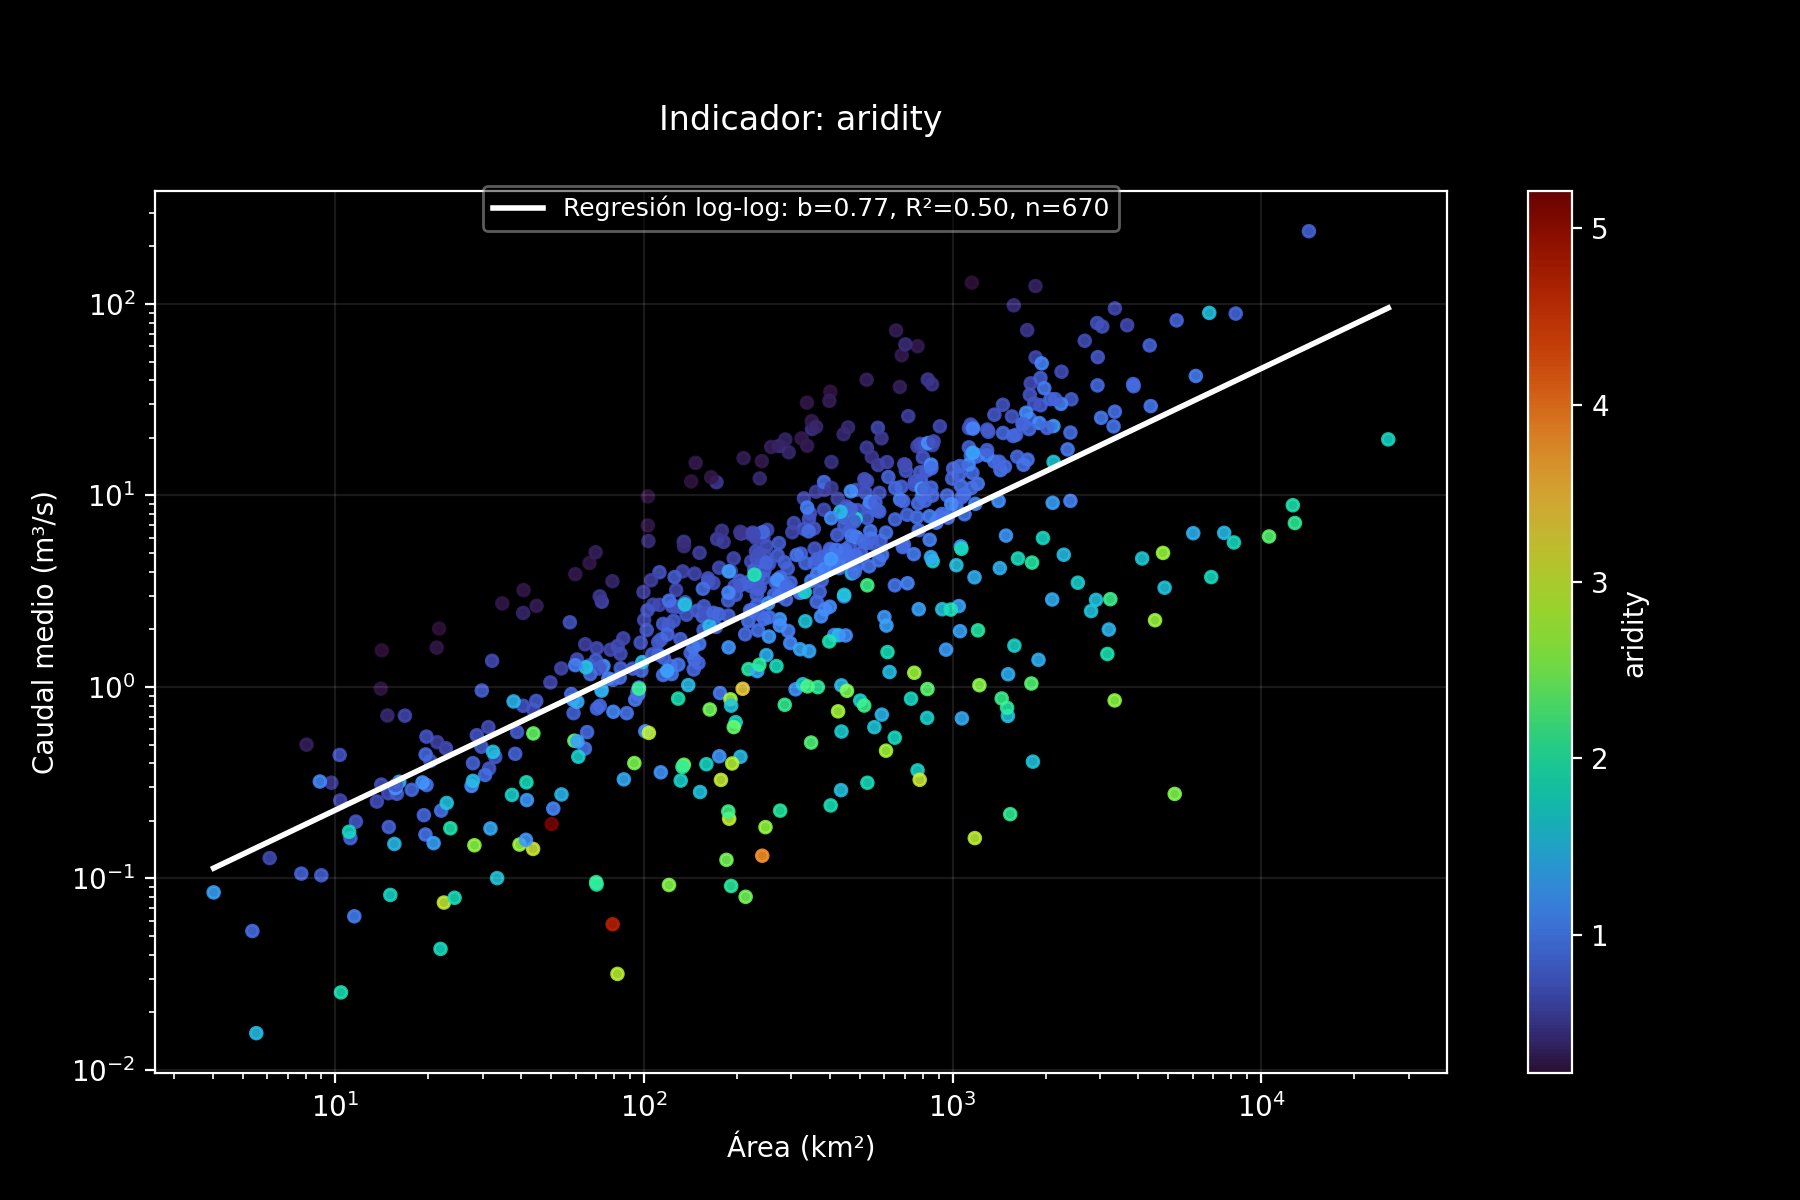
\includegraphics[width=0.48\textwidth]{../figuras/camels_area_vs_q_aridity.png}
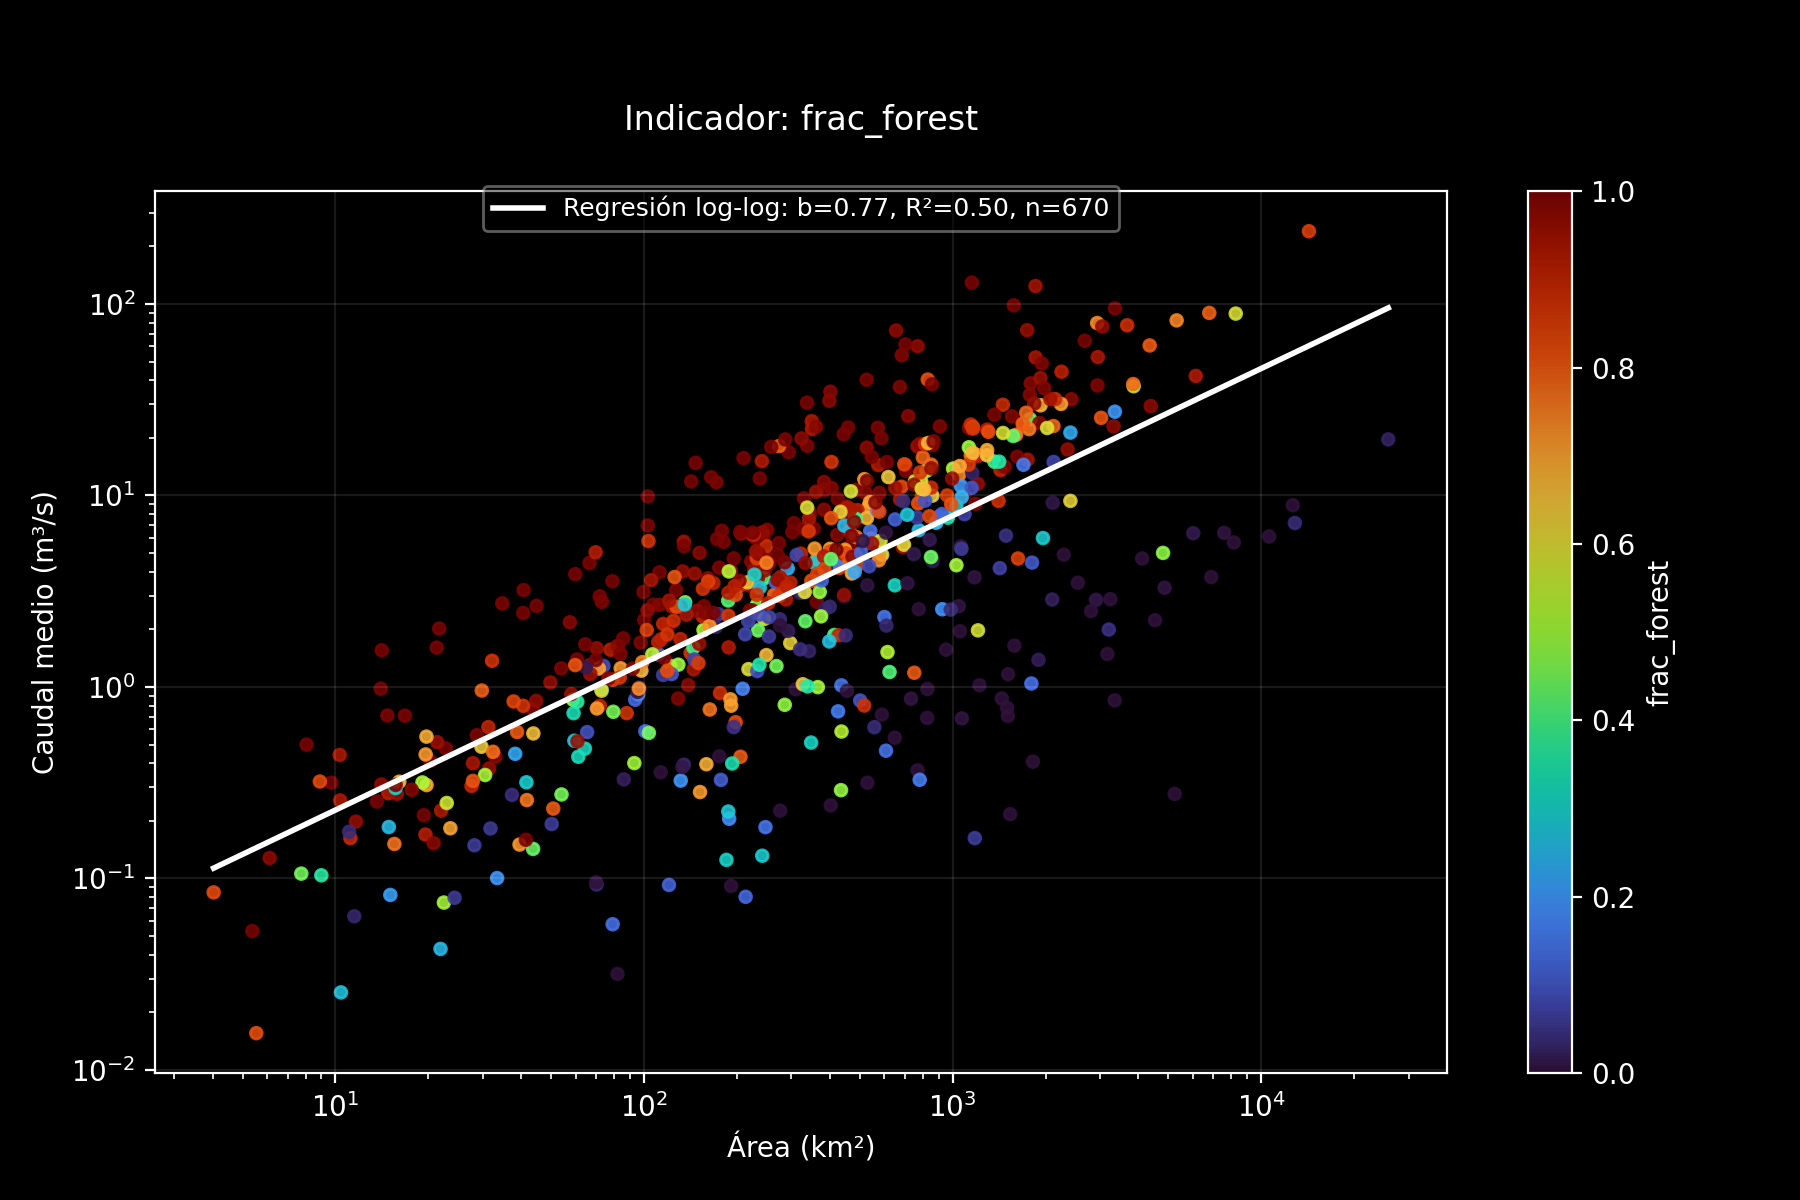
\includegraphics[width=0.48\textwidth]{../figuras/camels_area_vs_q_frac_forest.png}
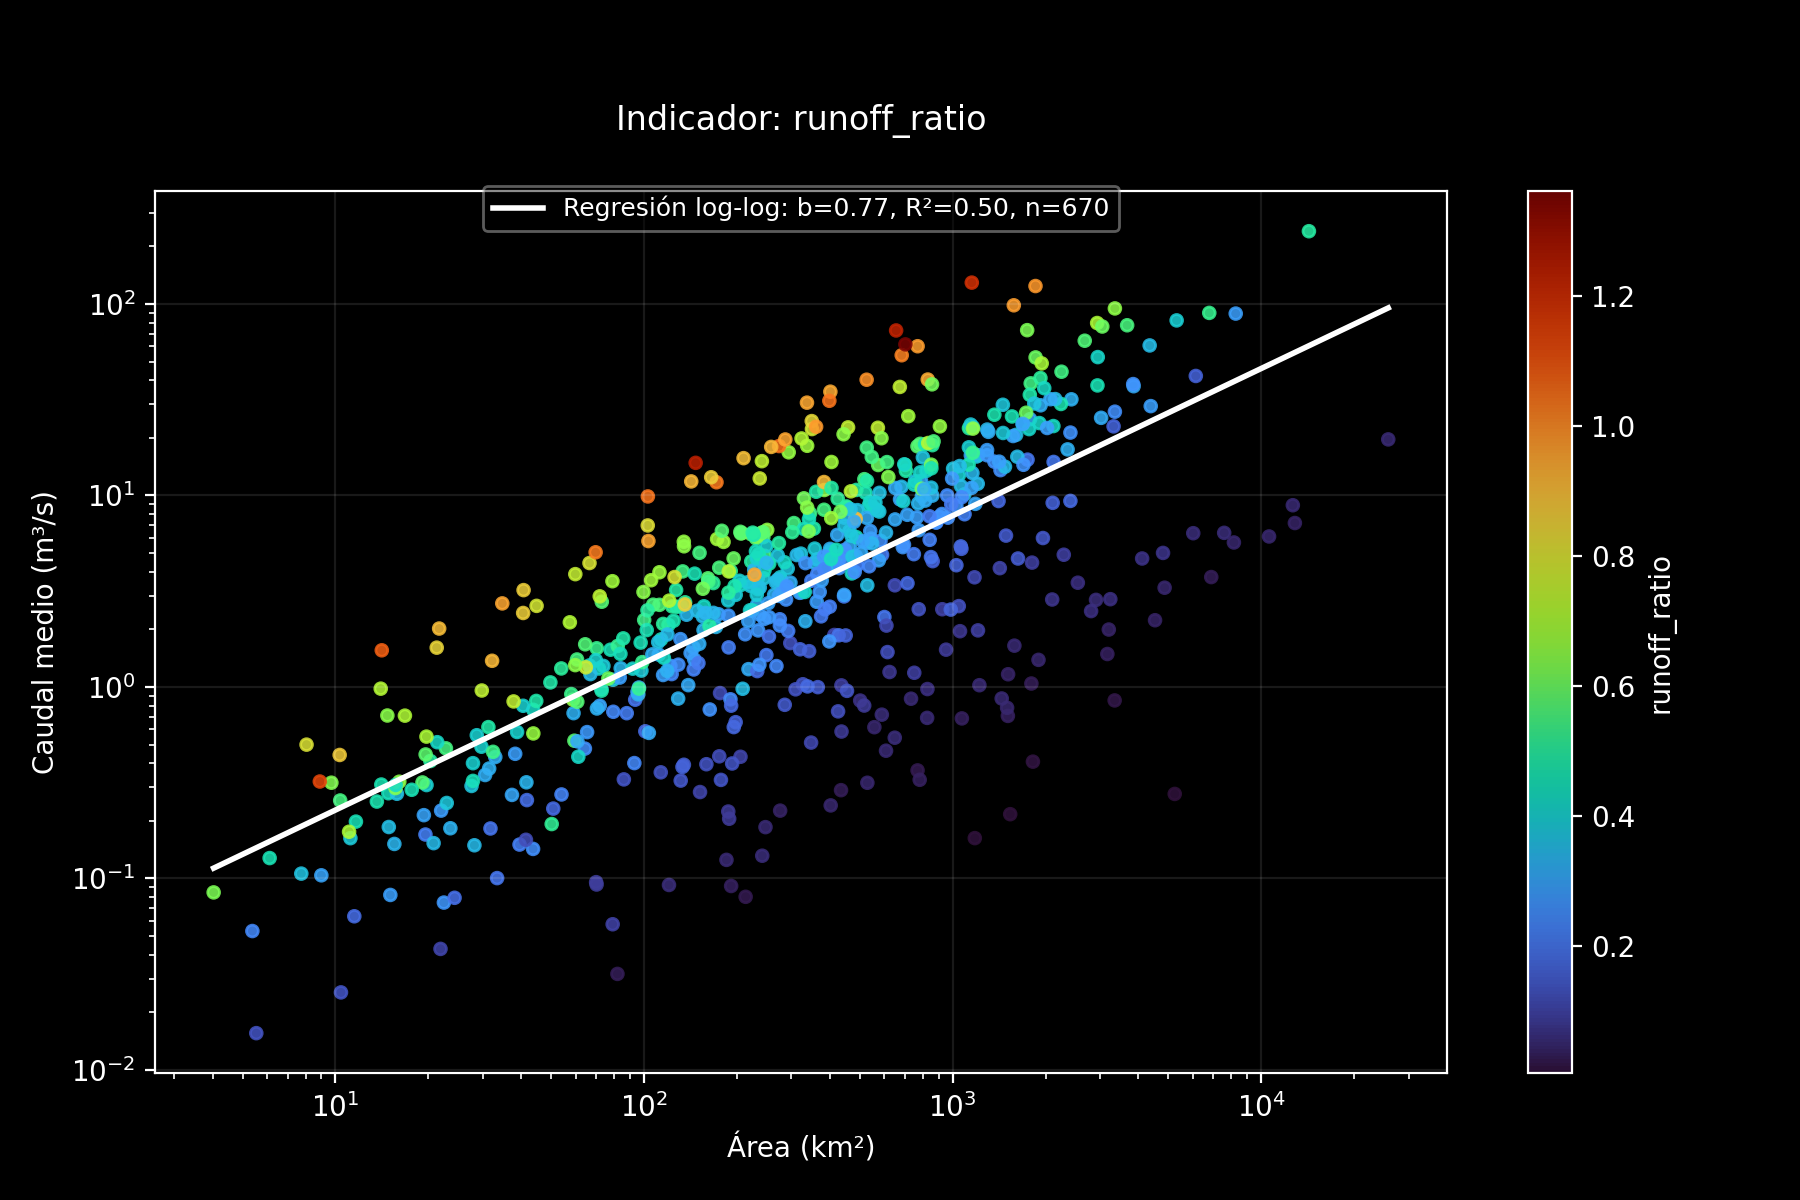
\includegraphics[width=0.48\textwidth]{../figuras/camels_area_vs_q_runoff_ratio.png}
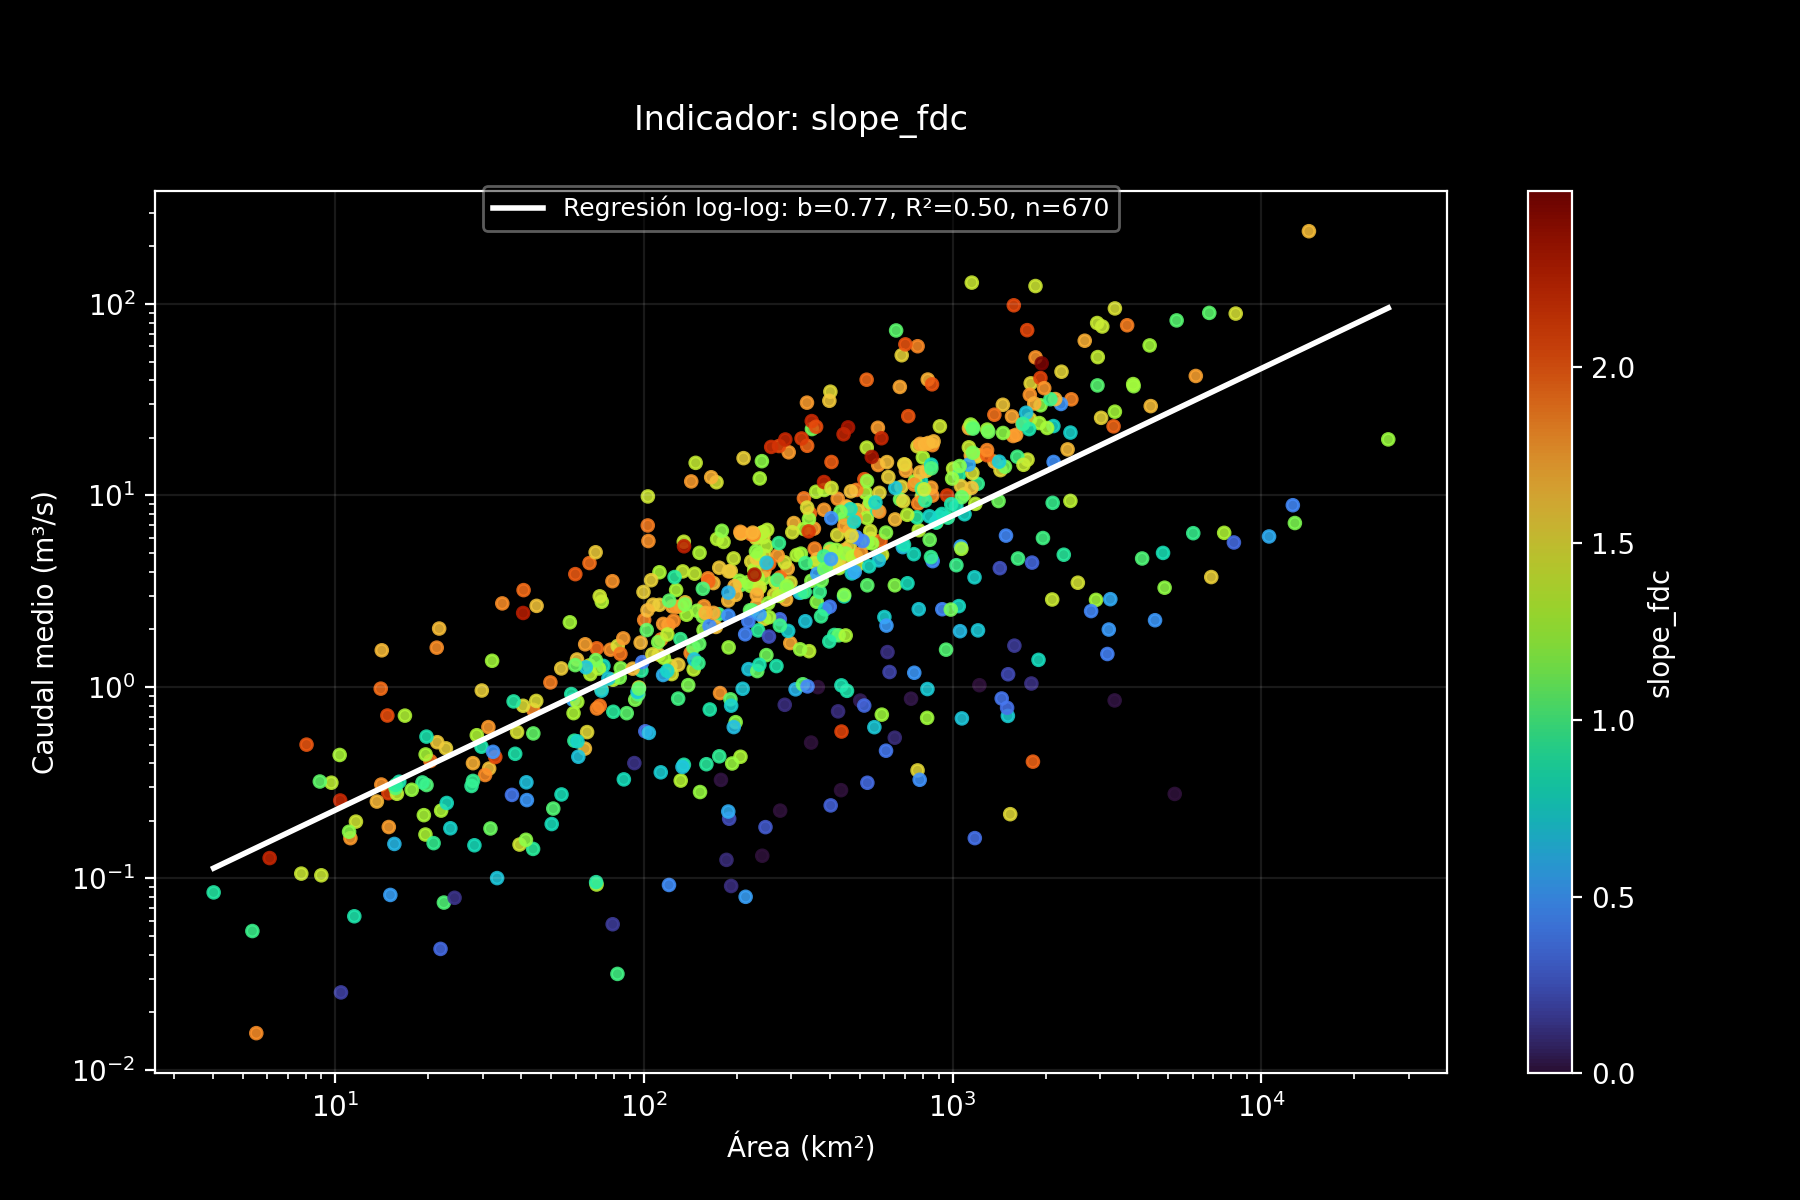
\includegraphics[width=0.48\textwidth]{../figuras/camels_area_vs_q_slope_fdc.png}
\caption{Dispersion area vs caudal medio (escala log-log) coloreada por distintos indicadores.}
\end{figure}

La base de datos CAMELS contiene 671 cuencas. Sin embargo, el ajuste de la relacion log--log entre area y caudal medio se realizo sobre 670 cuencas validas. La estacion 03281100 fue excluida debido a la presencia de valor faltante en la variable q\_mean, lo que genero un valor NaN en la variable derivada q\_mean\_cms. De esta manera, la regresion se estimo unicamente con registros completos y consistentes.

\begin{figure}[H]
\centering
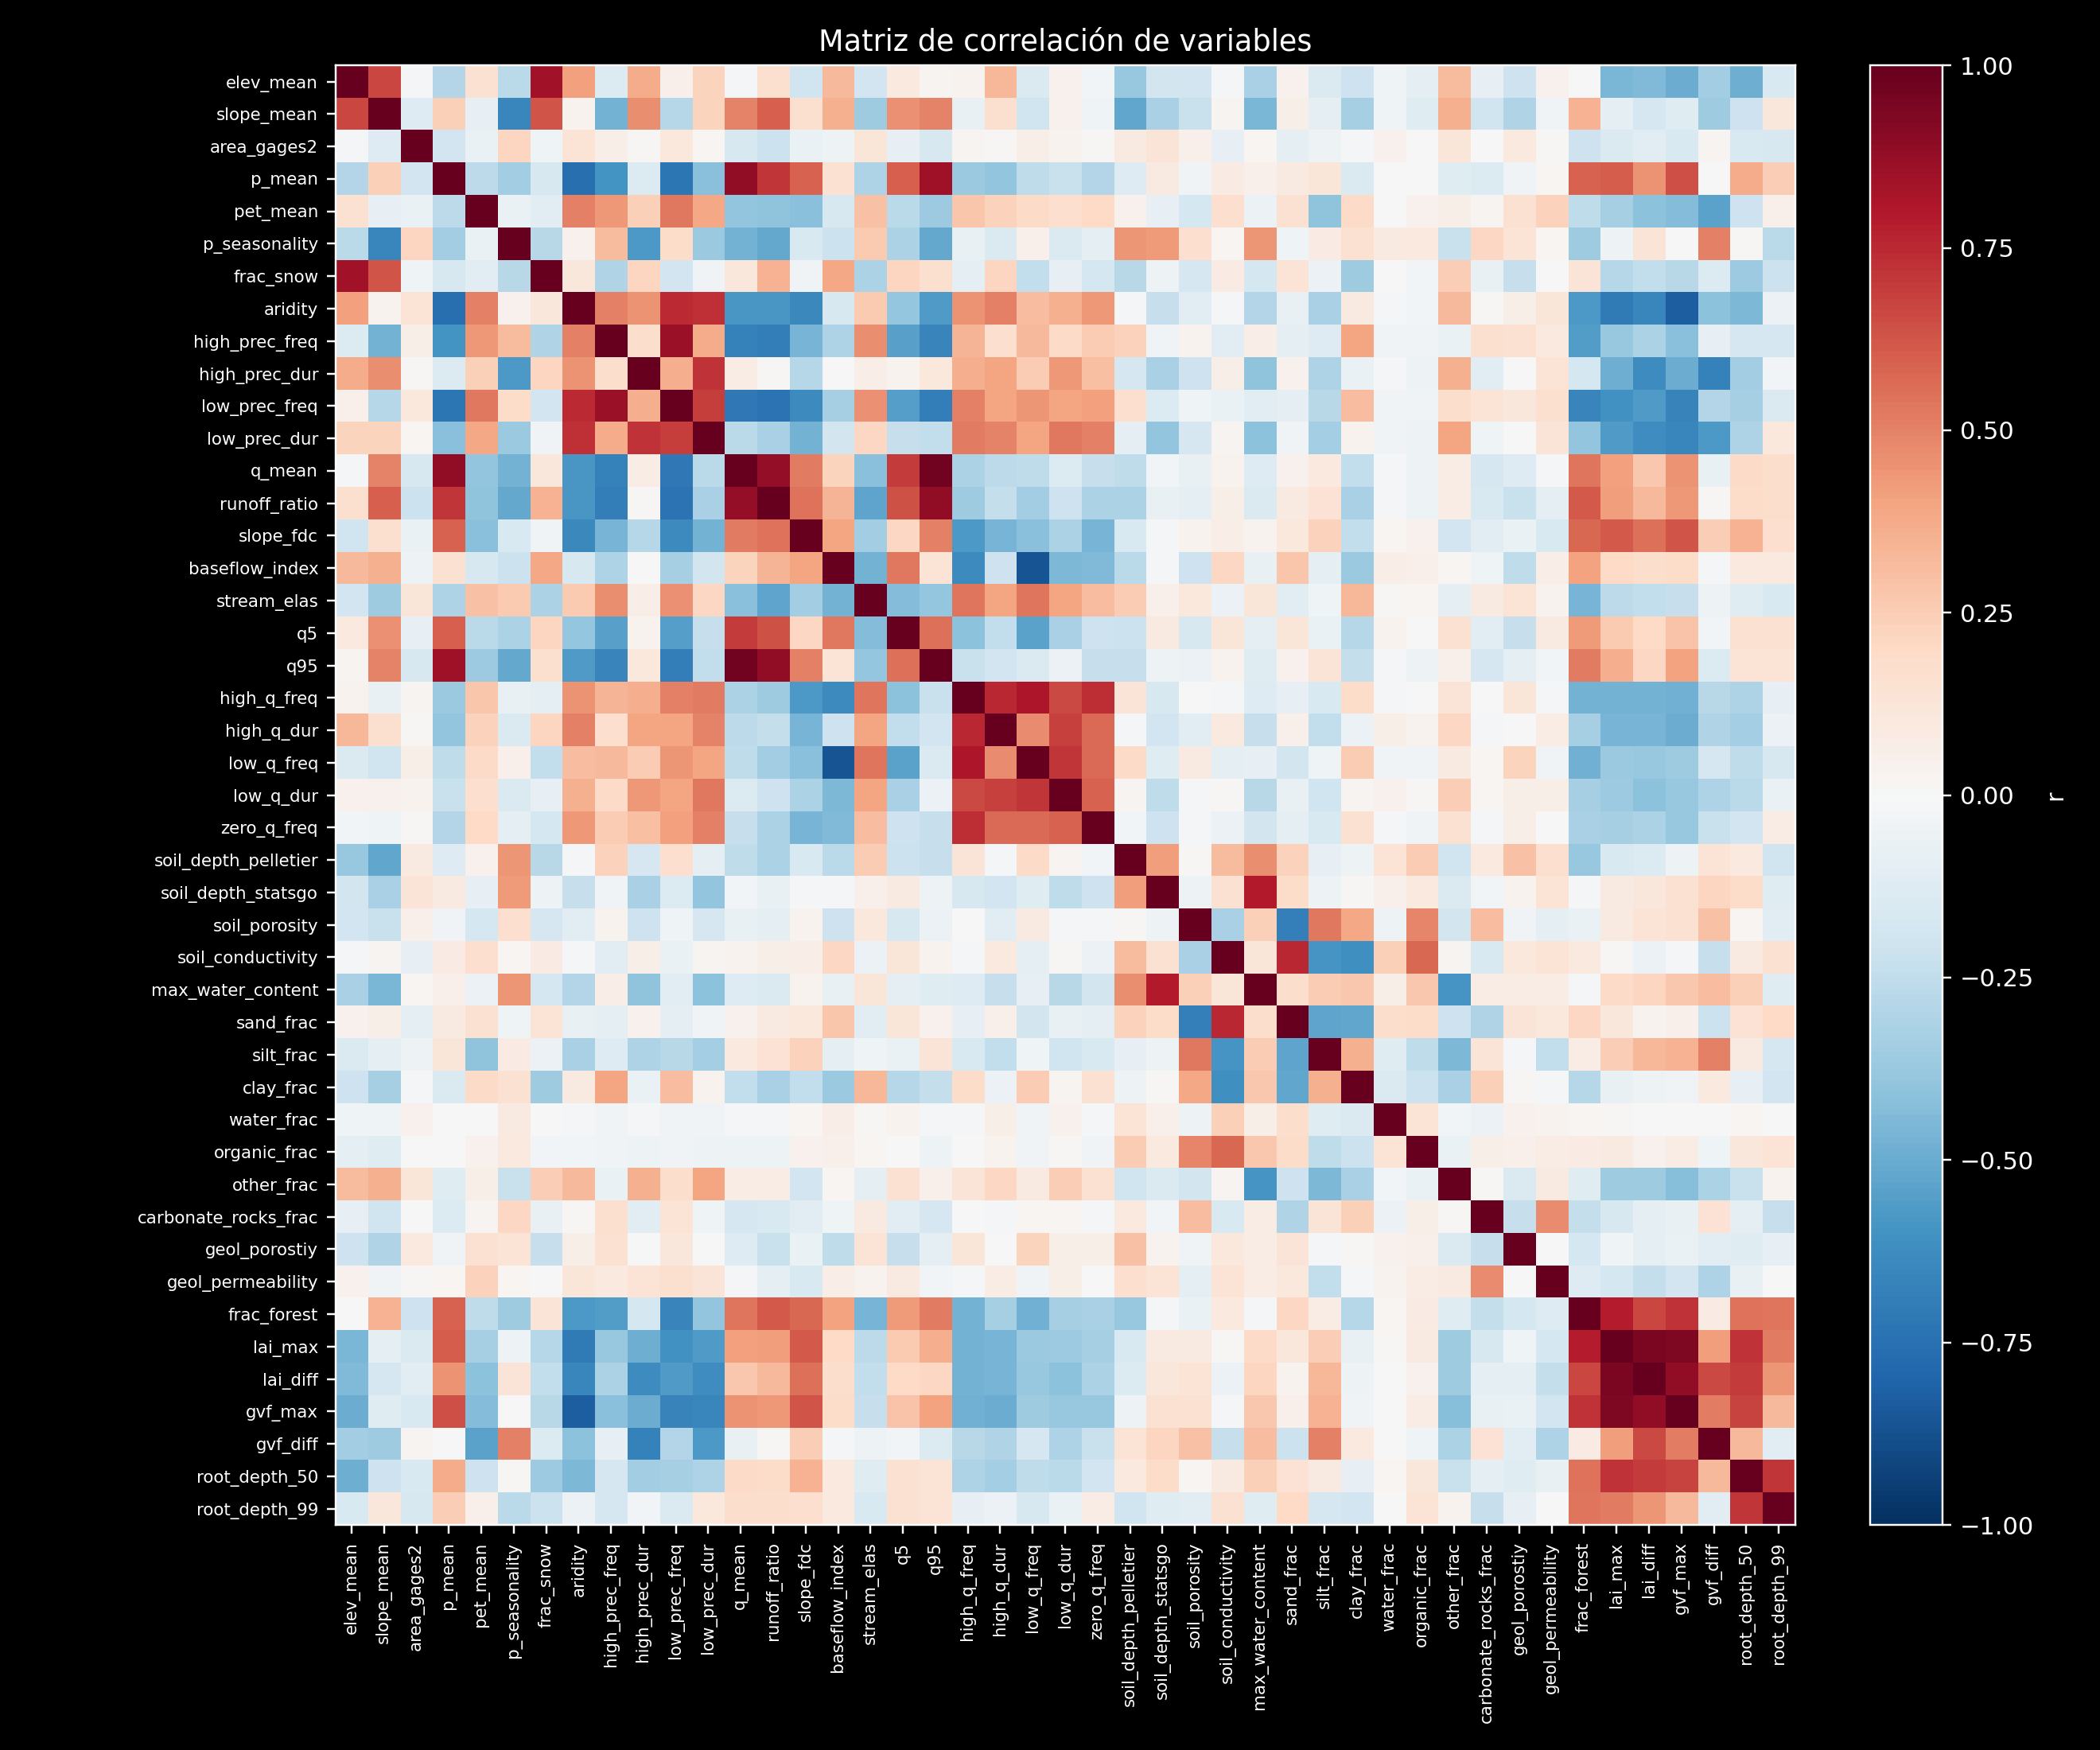
\includegraphics[width=0.85\textwidth]{../figuras/camels_correlacion_heatmap.png}
\caption{Matriz de correlacion entre variables de clima, suelo, geologia e hidrologia.}
\end{figure}

\textbf{Analisis de colinealidad entre atributos}

La matriz de correlacion evidencia la presencia de colinealidad significativa entre varios atributos hidrologicos y climaticos. En particular:
\begin{itemize}
\item runoff\_ratio y q\_mean presentan alta correlacion positiva, coherente con el control directo de la escorrentia sobre el caudal medio.
\item p\_mean y aridity muestran correlacion inversa marcada, consistente con la definicion del indice de aridez.
\item frac\_forest presenta correlaciones relevantes con variables climaticas, indicando influencia del regimen hidroclimatico regional.
\end{itemize}
Estas dependencias implican que los atributos no pueden interpretarse como factores independientes. Por lo tanto, las relaciones observadas deben analizarse considerando posibles efectos de control climatico subyacente y evitando interpretaciones causales simplificadas.

\subsection*{Parte 2 - Exploracion de datos}
Con el fin de comprender el comportamiento hidrologico previo a la modelacion, se realizo un analisis exploratorio de las series diarias y mensuales de precipitacion y caudal. Esta evaluacion permite identificar el regimen climatico dominante, la respuesta hidrologica de la cuenca y la consistencia entre diferentes fuentes meteorologicas utilizadas posteriormente en la calibracion.

\begin{figure}[H]
\centering
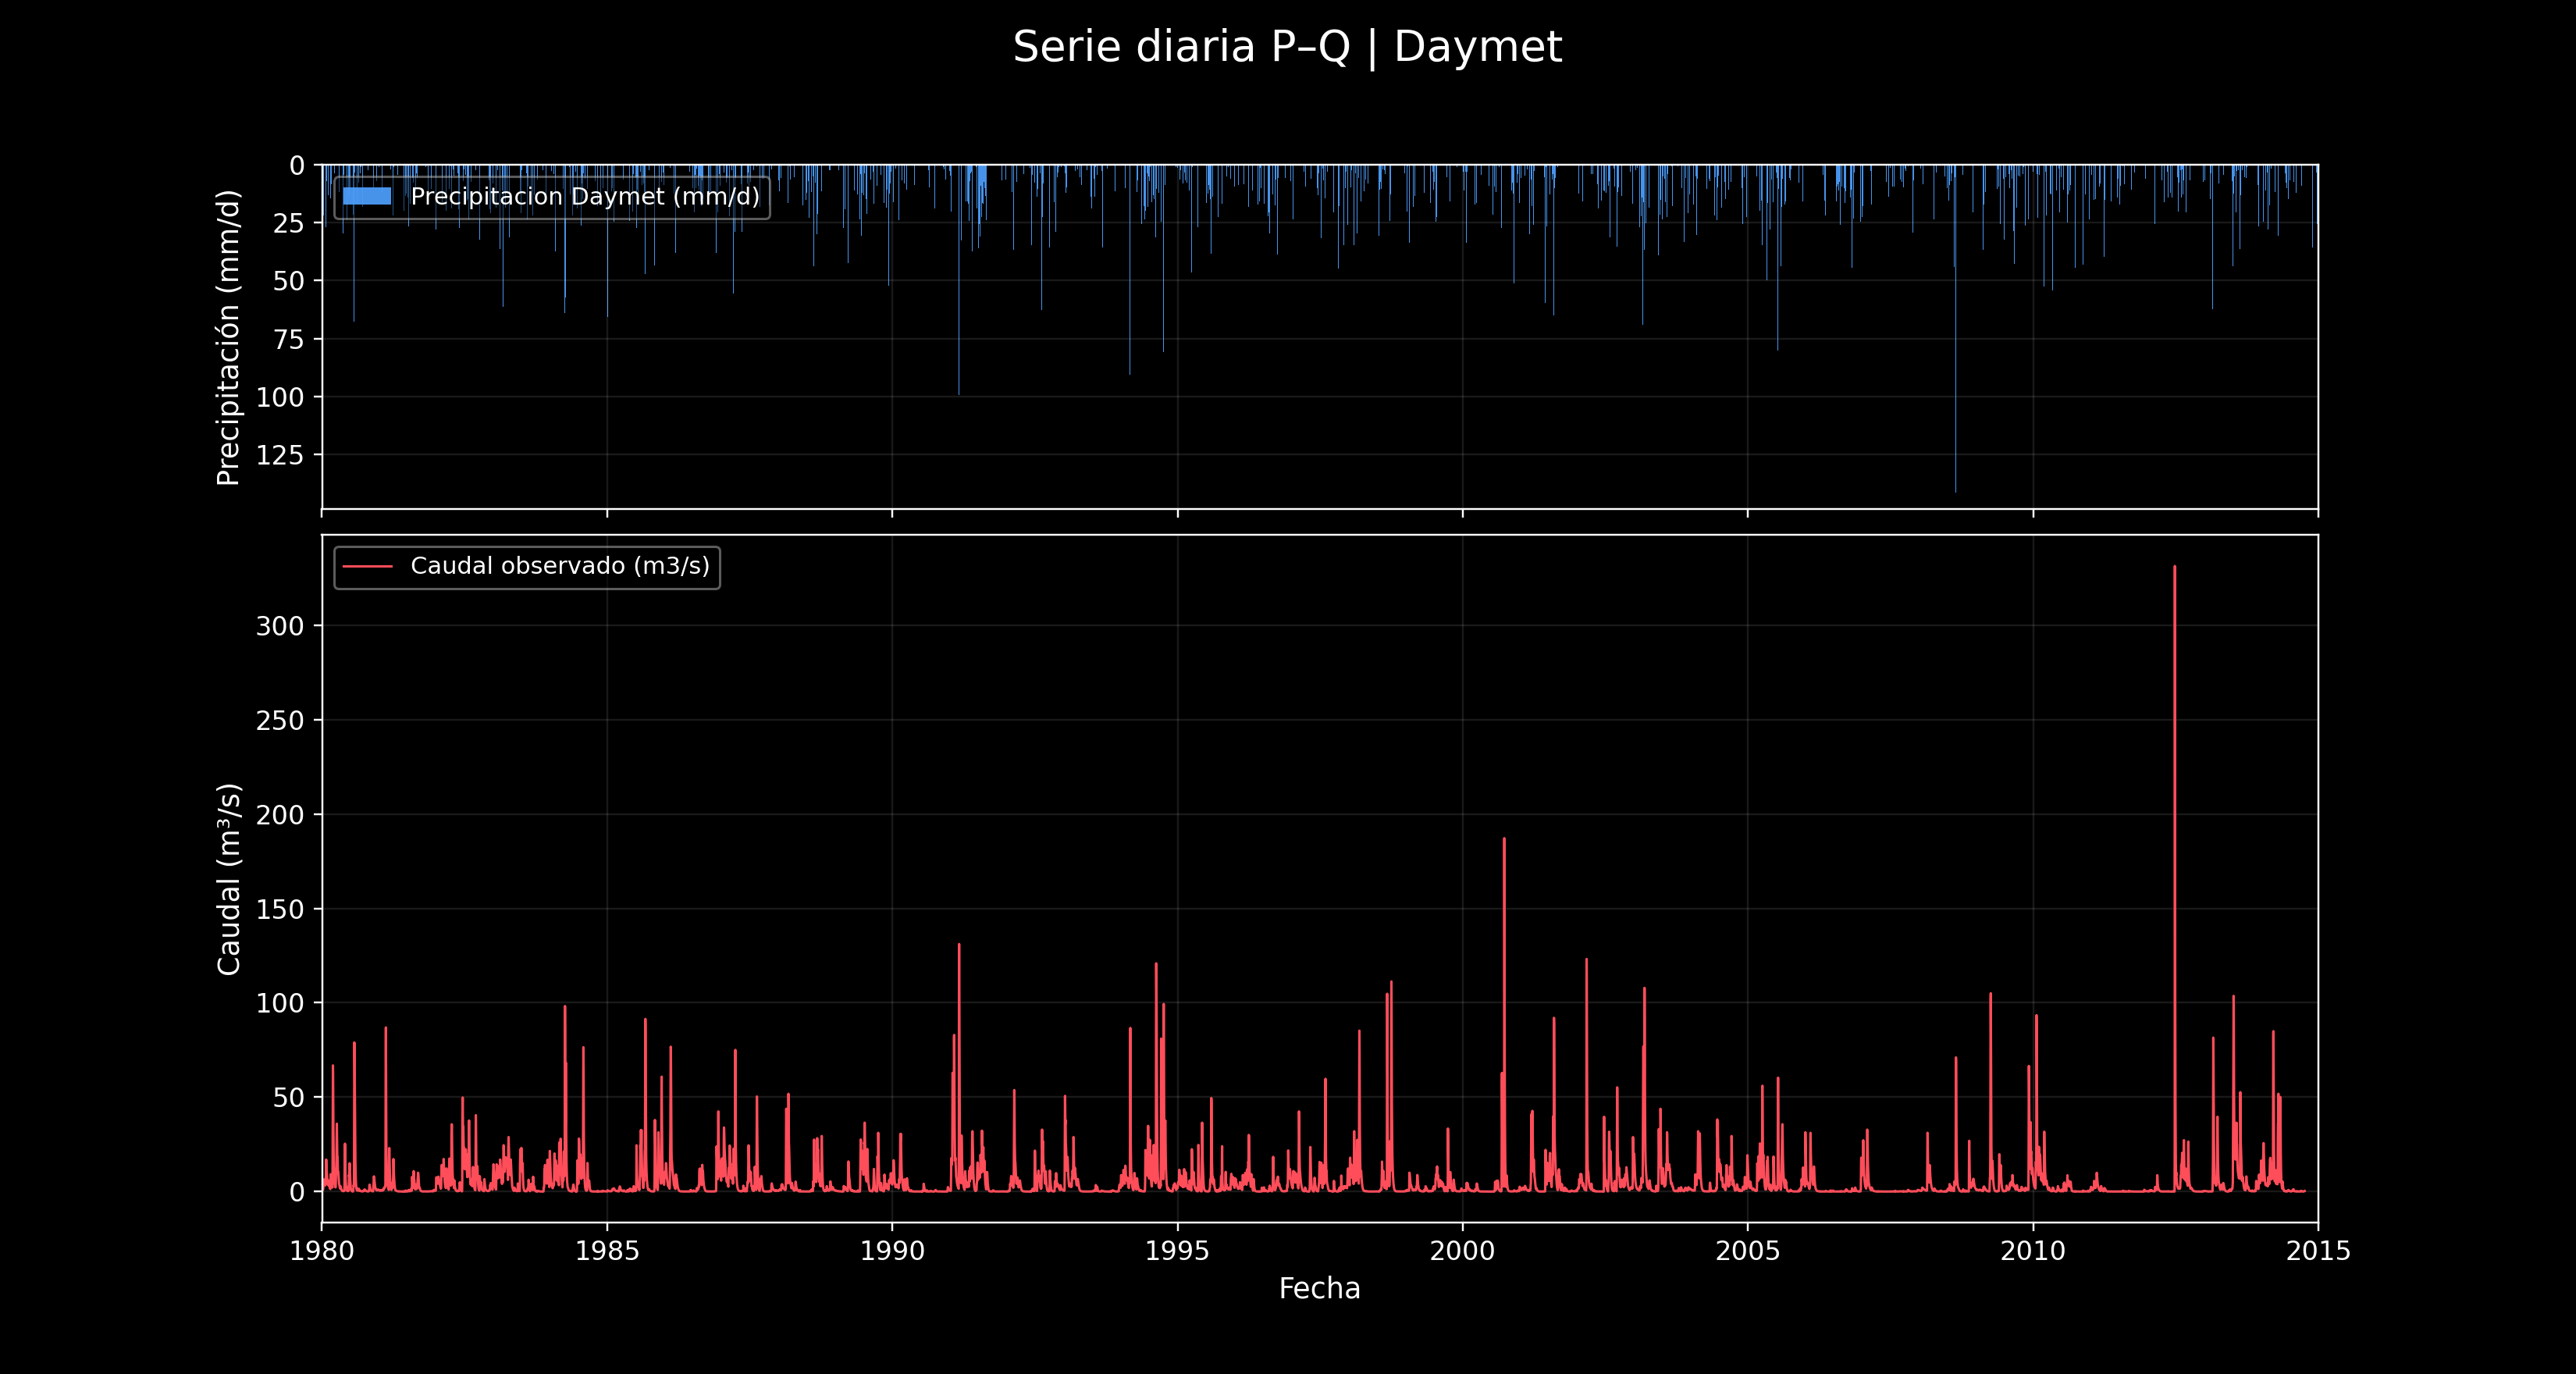
\includegraphics[width=0.95\textwidth]{../figuras/series_tiempo.png}
\caption{Serie diaria P-Q con Daymet (P invertida en panel superior).}
\end{figure}

La serie diaria de precipitacion y caudal muestra un regimen predominantemente pluvial, sin evidencia de estacionalidad asociada a nieve. Se observan eventos de precipitacion frecuentes a lo largo del ano, con episodios de alta intensidad superiores a 100 mm/dia.

El caudal presenta una respuesta rapida ante eventos intensos de lluvia, indicando una componente relevante de escorrentia directa. Sin embargo, la presencia de un caudal base persistente sugiere una contribucion subterranea significativa, consistente con las caracteristicas hidroclimaticas de la region.

Se identifican eventos extremos aislados con picos superiores a 300 m$^3$/s, sin evidencia de regulacion artificial o discontinuidades estructurales en la serie.

\begin{figure}[H]
\centering
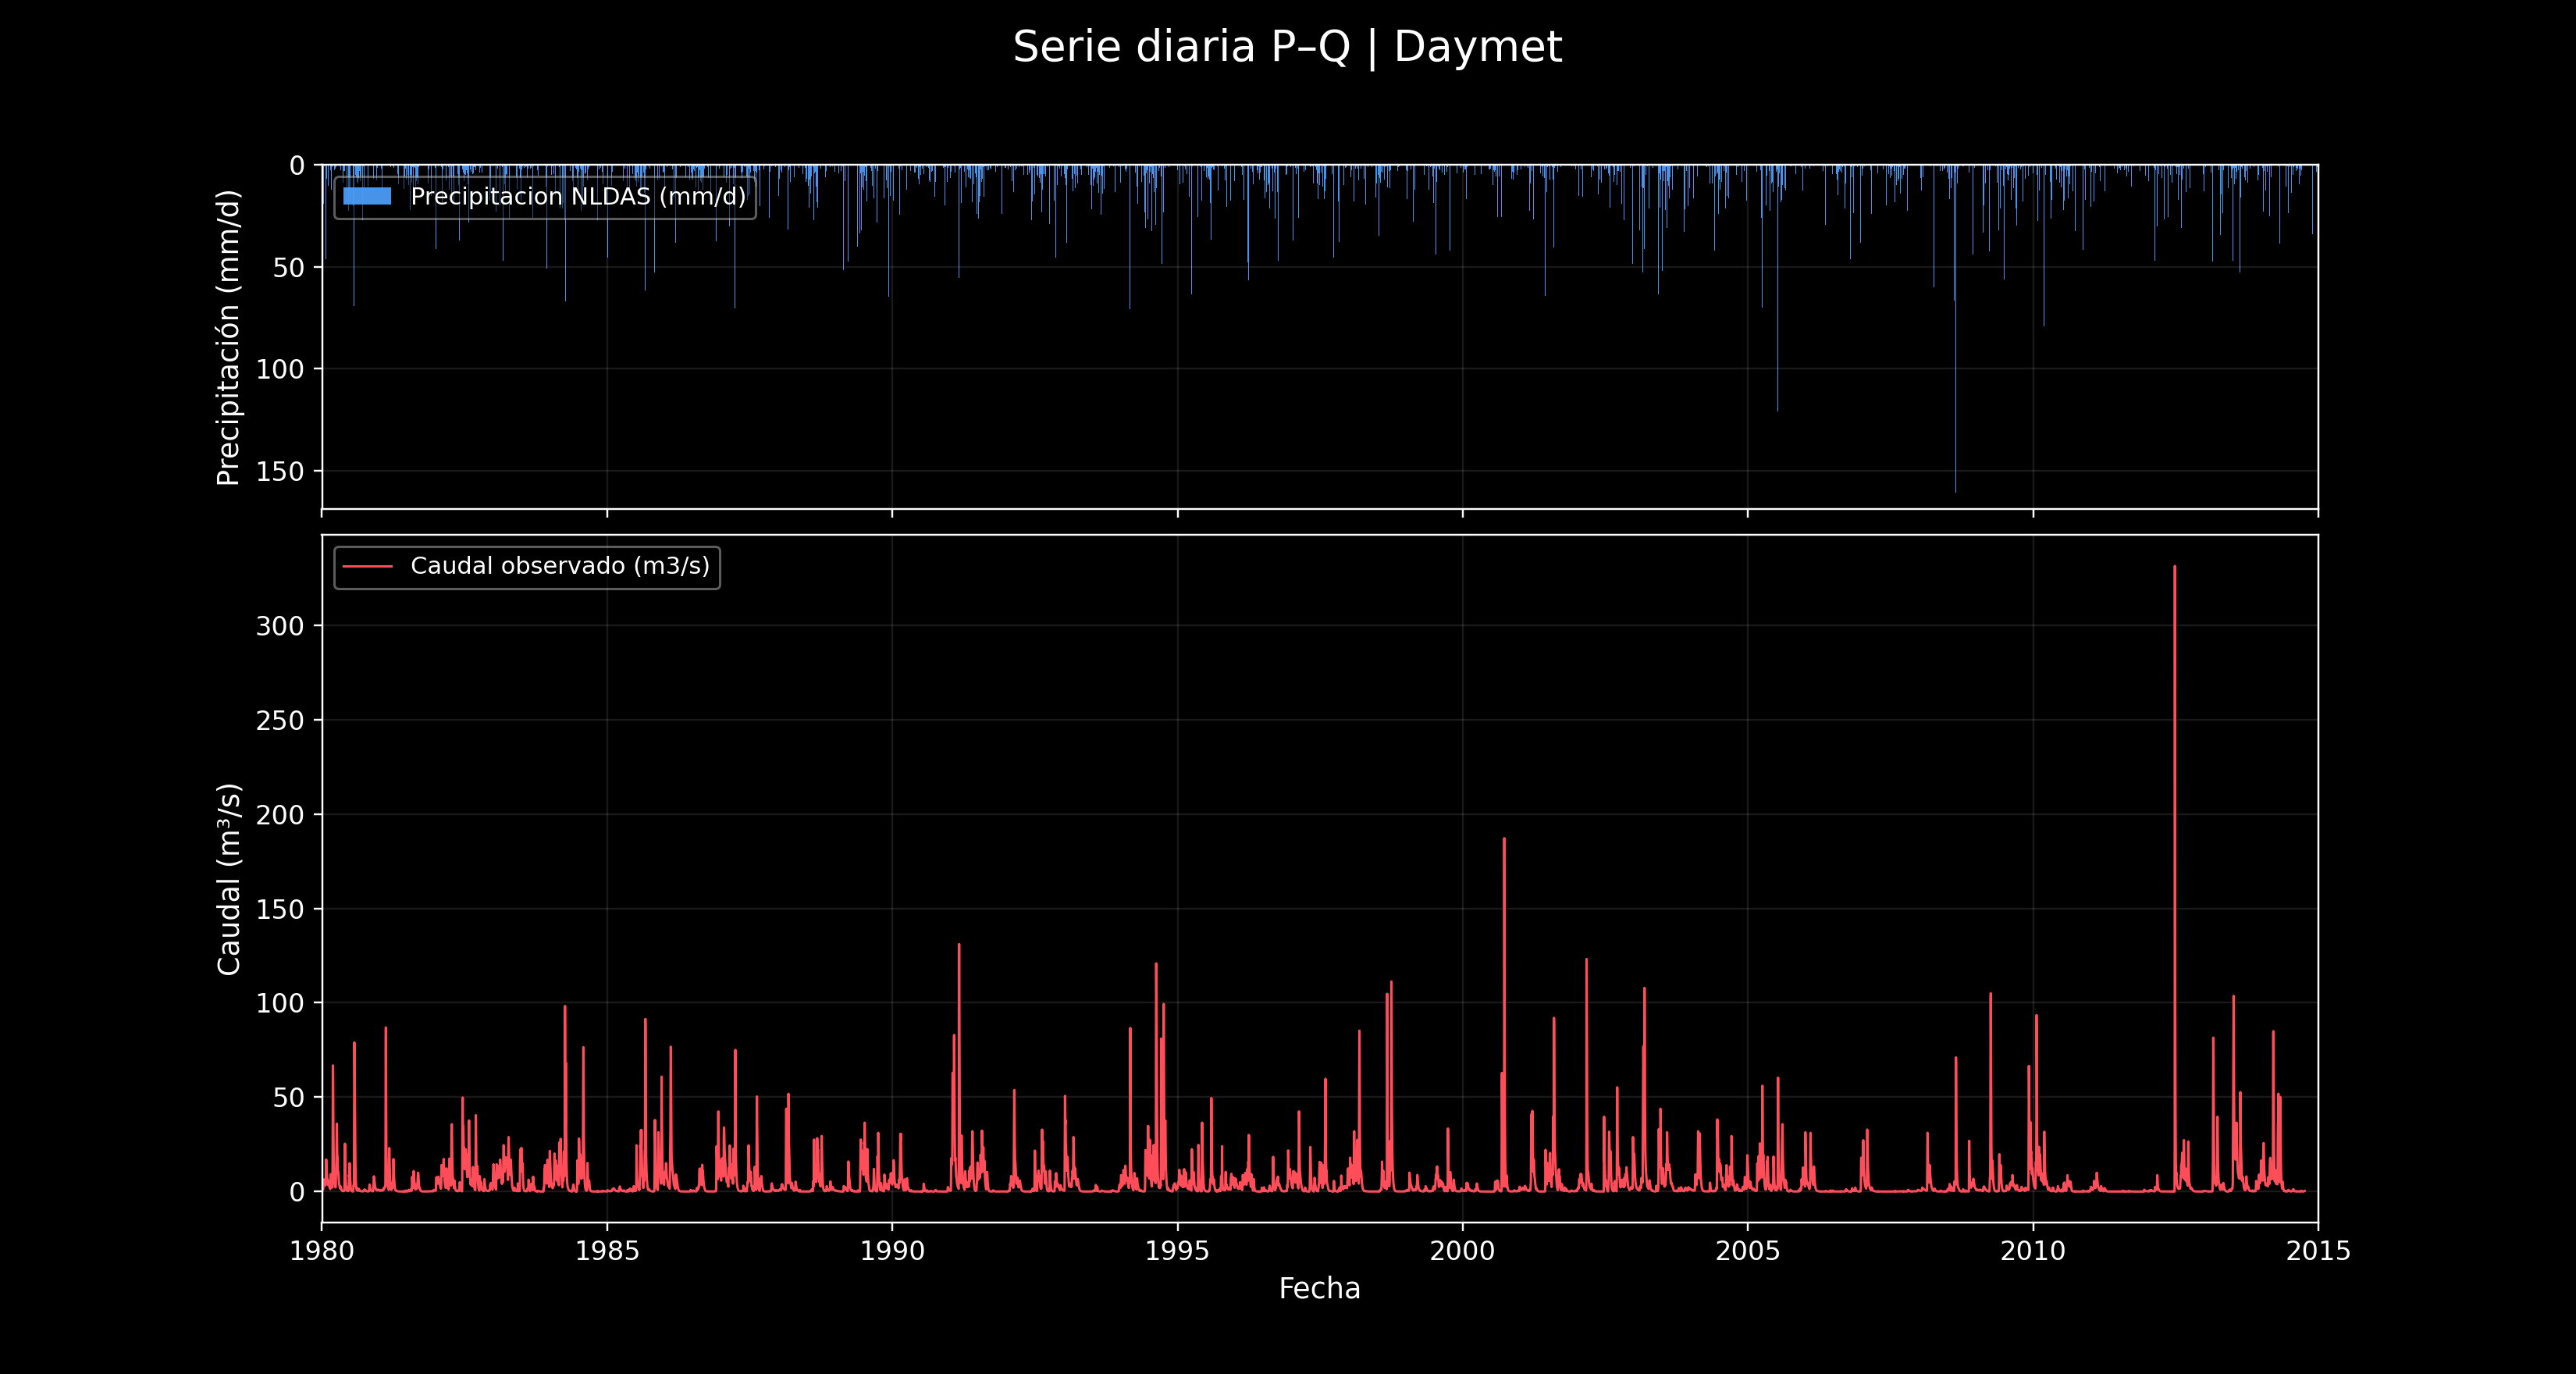
\includegraphics[width=0.95\textwidth]{../figuras/series_tiempo_nldas.png}
\caption{Serie diaria P-Q con NLDAS (P invertida en panel superior).}
\end{figure}

\begin{figure}[H]
\centering
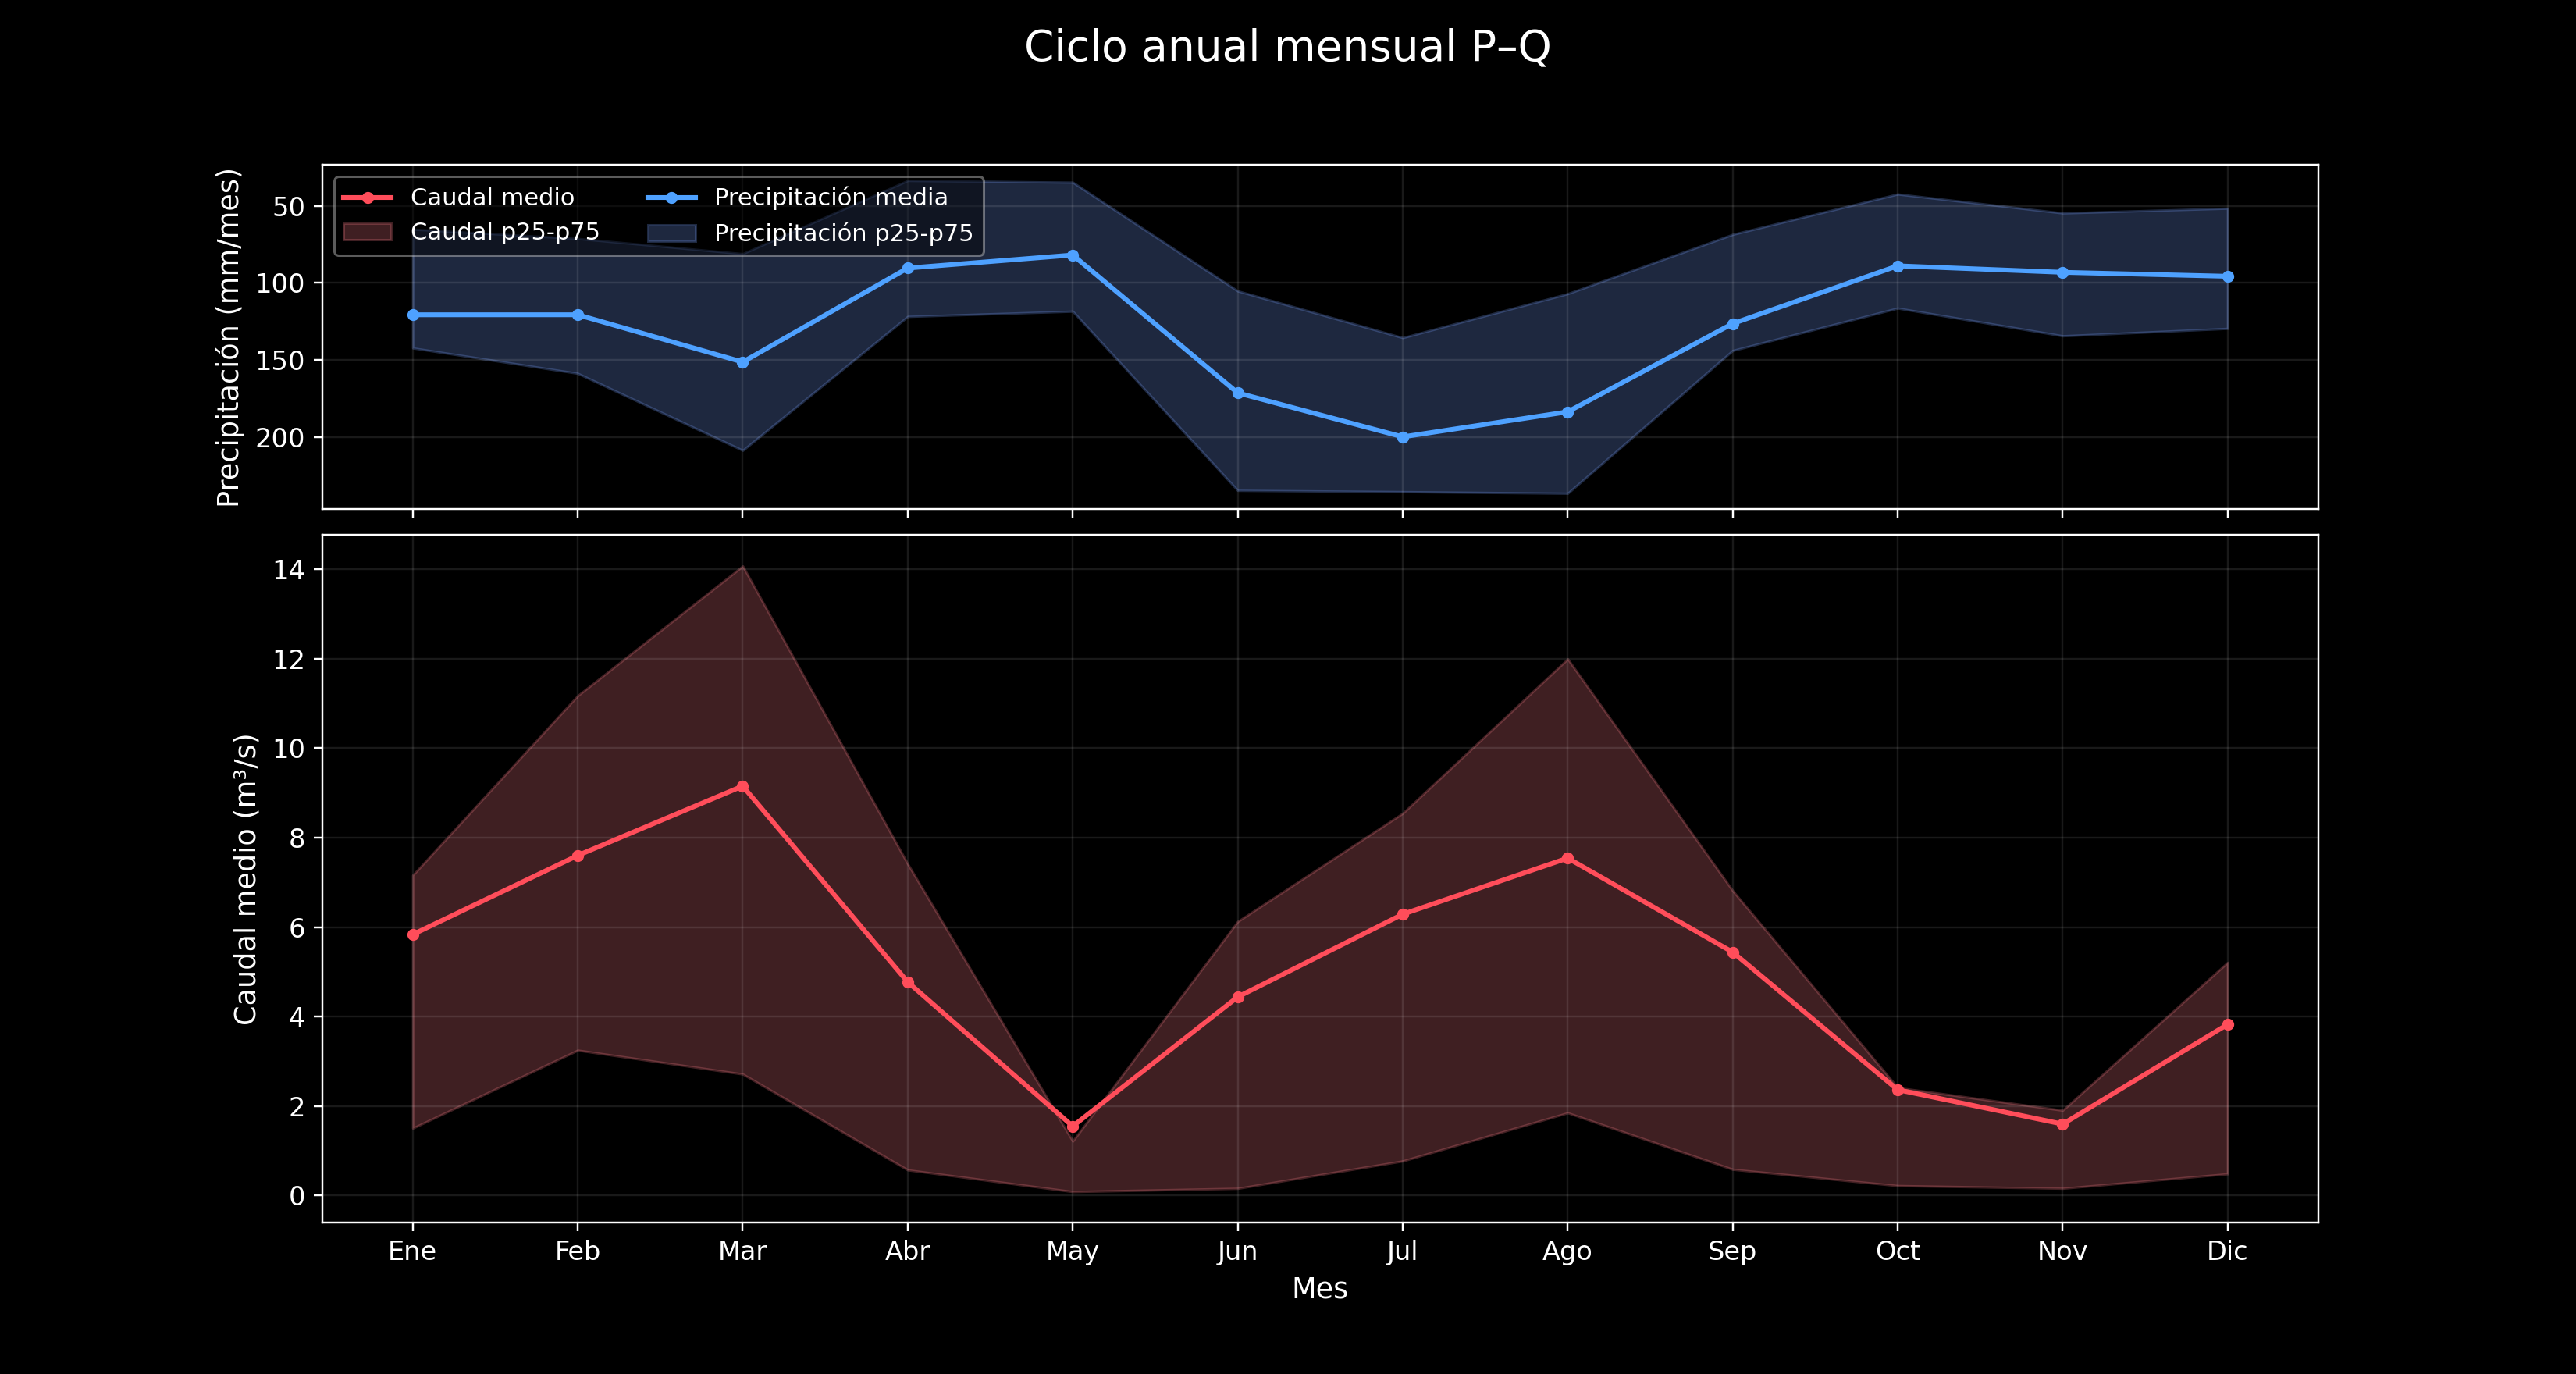
\includegraphics[width=0.80\textwidth]{../figuras/ciclo_anual.png}
\caption{Ciclo anual mensual de precipitacion y caudal (media y banda P25-P75).}
\end{figure}

El ciclo anual mensual revela un patron estacional bien definido. La precipitacion presenta maximos durante el verano (julio--septiembre) y valores relativamente menores durante la primavera.

No obstante, el caudal medio mensual no coincide exactamente con los maximos de precipitacion. Se observa un maximo principal en febrero--marzo y un segundo maximo en agosto, mientras que el minimo ocurre en mayo.

Este desfase entre precipitacion y caudal sugiere la presencia de almacenamiento intermedio y control evaporativo, particularmente durante los meses de verano, cuando la evapotranspiracion potencial es elevada. La amplitud del rango intercuartilico (p25--p75) indica ademas alta variabilidad interanual.

Este comportamiento justifica la utilizacion de un modelo conceptual con almacenamiento multiple, como el modelo de dos tanques implementado en este estudio. La cuenca no responde instantaneamente al regimen de precipitacion mensual; existe modulacion climatica y almacenamiento interno.

\begin{figure}[H]
\centering
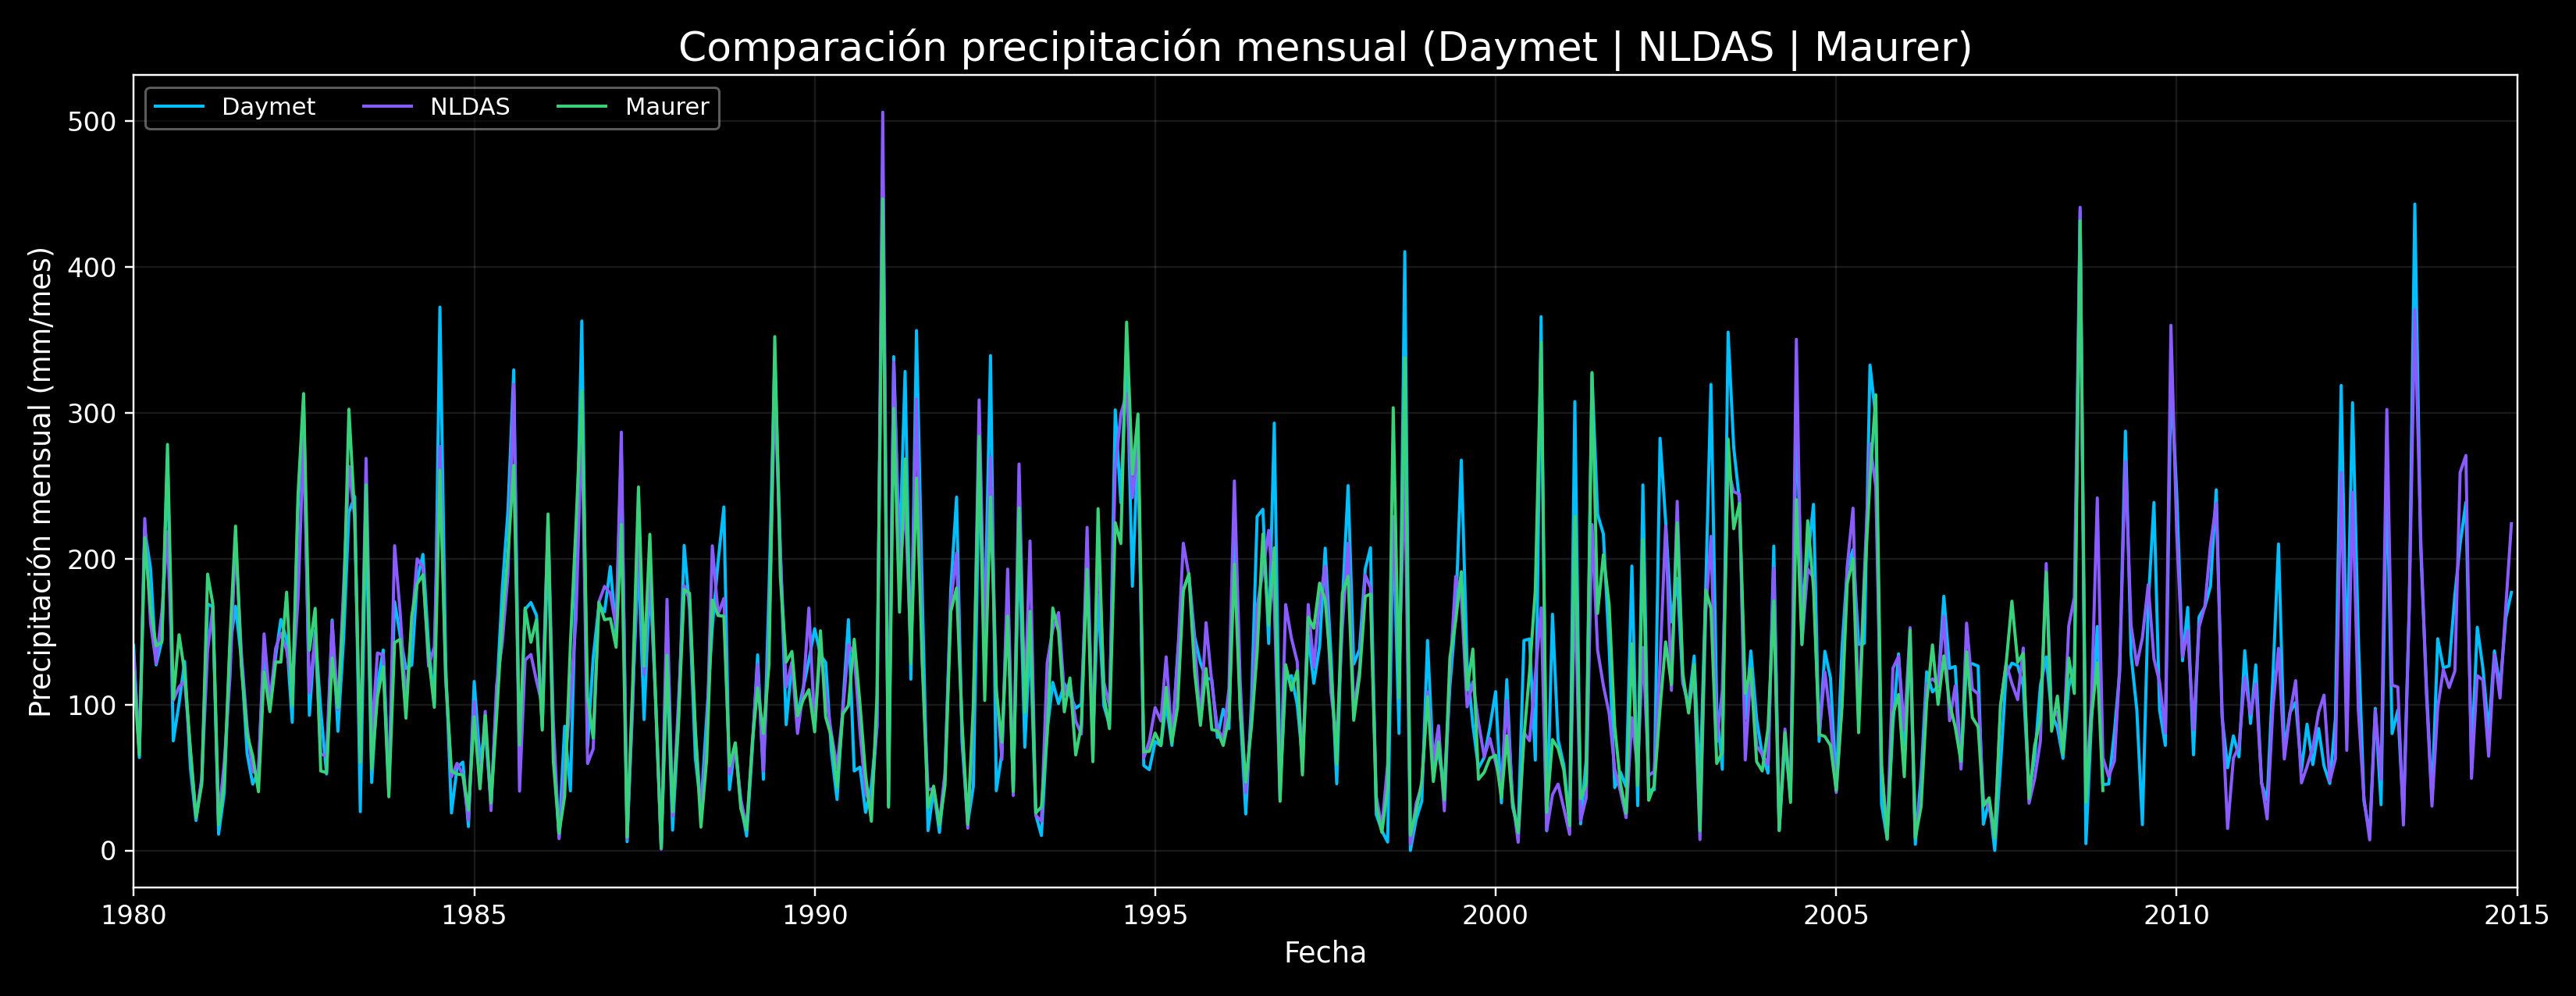
\includegraphics[width=0.90\textwidth]{../figuras/comparacion_precip.png}
\caption{Comparacion de precipitacion mensual Daymet, NLDAS y Maurer.}
\end{figure}

La comparacion visual entre Daymet y NLDAS a escala diaria muestra patrones temporales altamente consistentes, con coincidencia en la ocurrencia de eventos y estacionalidad general. Las diferencias se observan principalmente en la magnitud puntual de algunos eventos extremos.

A escala mensual, Daymet, NLDAS y Maurer presentan alta consistencia en la representacion de la variabilidad interanual y estacional. Sin embargo, Maurer presenta un periodo temporal mas corto (hasta 2008). Para mantener consistencia temporal en los periodos de calibracion (1990--1999) y validacion (2000--2009), se decidio utilizar exclusivamente Daymet y NLDAS en la implementacion del modelo hidrologico.

\begin{table}[H]
        \centering
        \scriptsize
        \caption{Estadísticas básicas de variables hidrometeorológicas}
        \label{tab:stats}
        \resizebox{\textwidth}{!}{%
        \begin{tabular}{lllllllll}
\toprule
Variable & Unidades & N & Missing & Media & DesvStd & Max & P25 & P75 \\
\midrule
prcp\_daymet\_mm\_day & mm/d & 12784.000 & 0.000 & 4.186 & 10.156 & 141.590 & 0.000 & 2.888 \\
prcp\_nldas\_mm\_day & mm/d & 12784.000 & 0.000 & 4.064 & 9.883 & 160.860 & 0.000 & 3.500 \\
prcp\_maurer\_mm\_day & mm/d & 10593.000 & 2191.000 & 3.975 & 8.568 & 128.260 & 0.000 & 4.150 \\
q\_m3s & m3/s & 12697.000 & 87.000 & 5.045 & 10.861 & 331.307 & 0.193 & 5.437 \\
\bottomrule
\end{tabular}

        }
        \end{table}

Las estadisticas confirman que Maurer presenta datos faltantes y menor cobertura temporal. La distribucion altamente asimetrica del caudal (media < maximo) refleja la naturaleza episodica de los eventos extremos.

\subsection*{Parte 3 - Implementacion del modelo}
Se implemento un modelo hidrologico conceptual de dos tanques en serie, conforme al enunciado del ejercicio. El modelo incluye dos estados de almacenamiento ($S_1$, $S_2$), desbordes controlados por umbrales ($D_1$, $D_2$) y descargas lentas reguladas por coeficientes ($k_1$, $k_2$). La precipitacion efectiva alimenta el primer tanque, y el caudal total resulta de la combinacion de descargas rapidas y lentas.

Previo al proceso de calibracion, se evaluo el desempeno del modelo utilizando parametros por defecto, con el fin de verificar estabilidad estructural y consistencia fisica.

\begin{figure}[H]
\centering
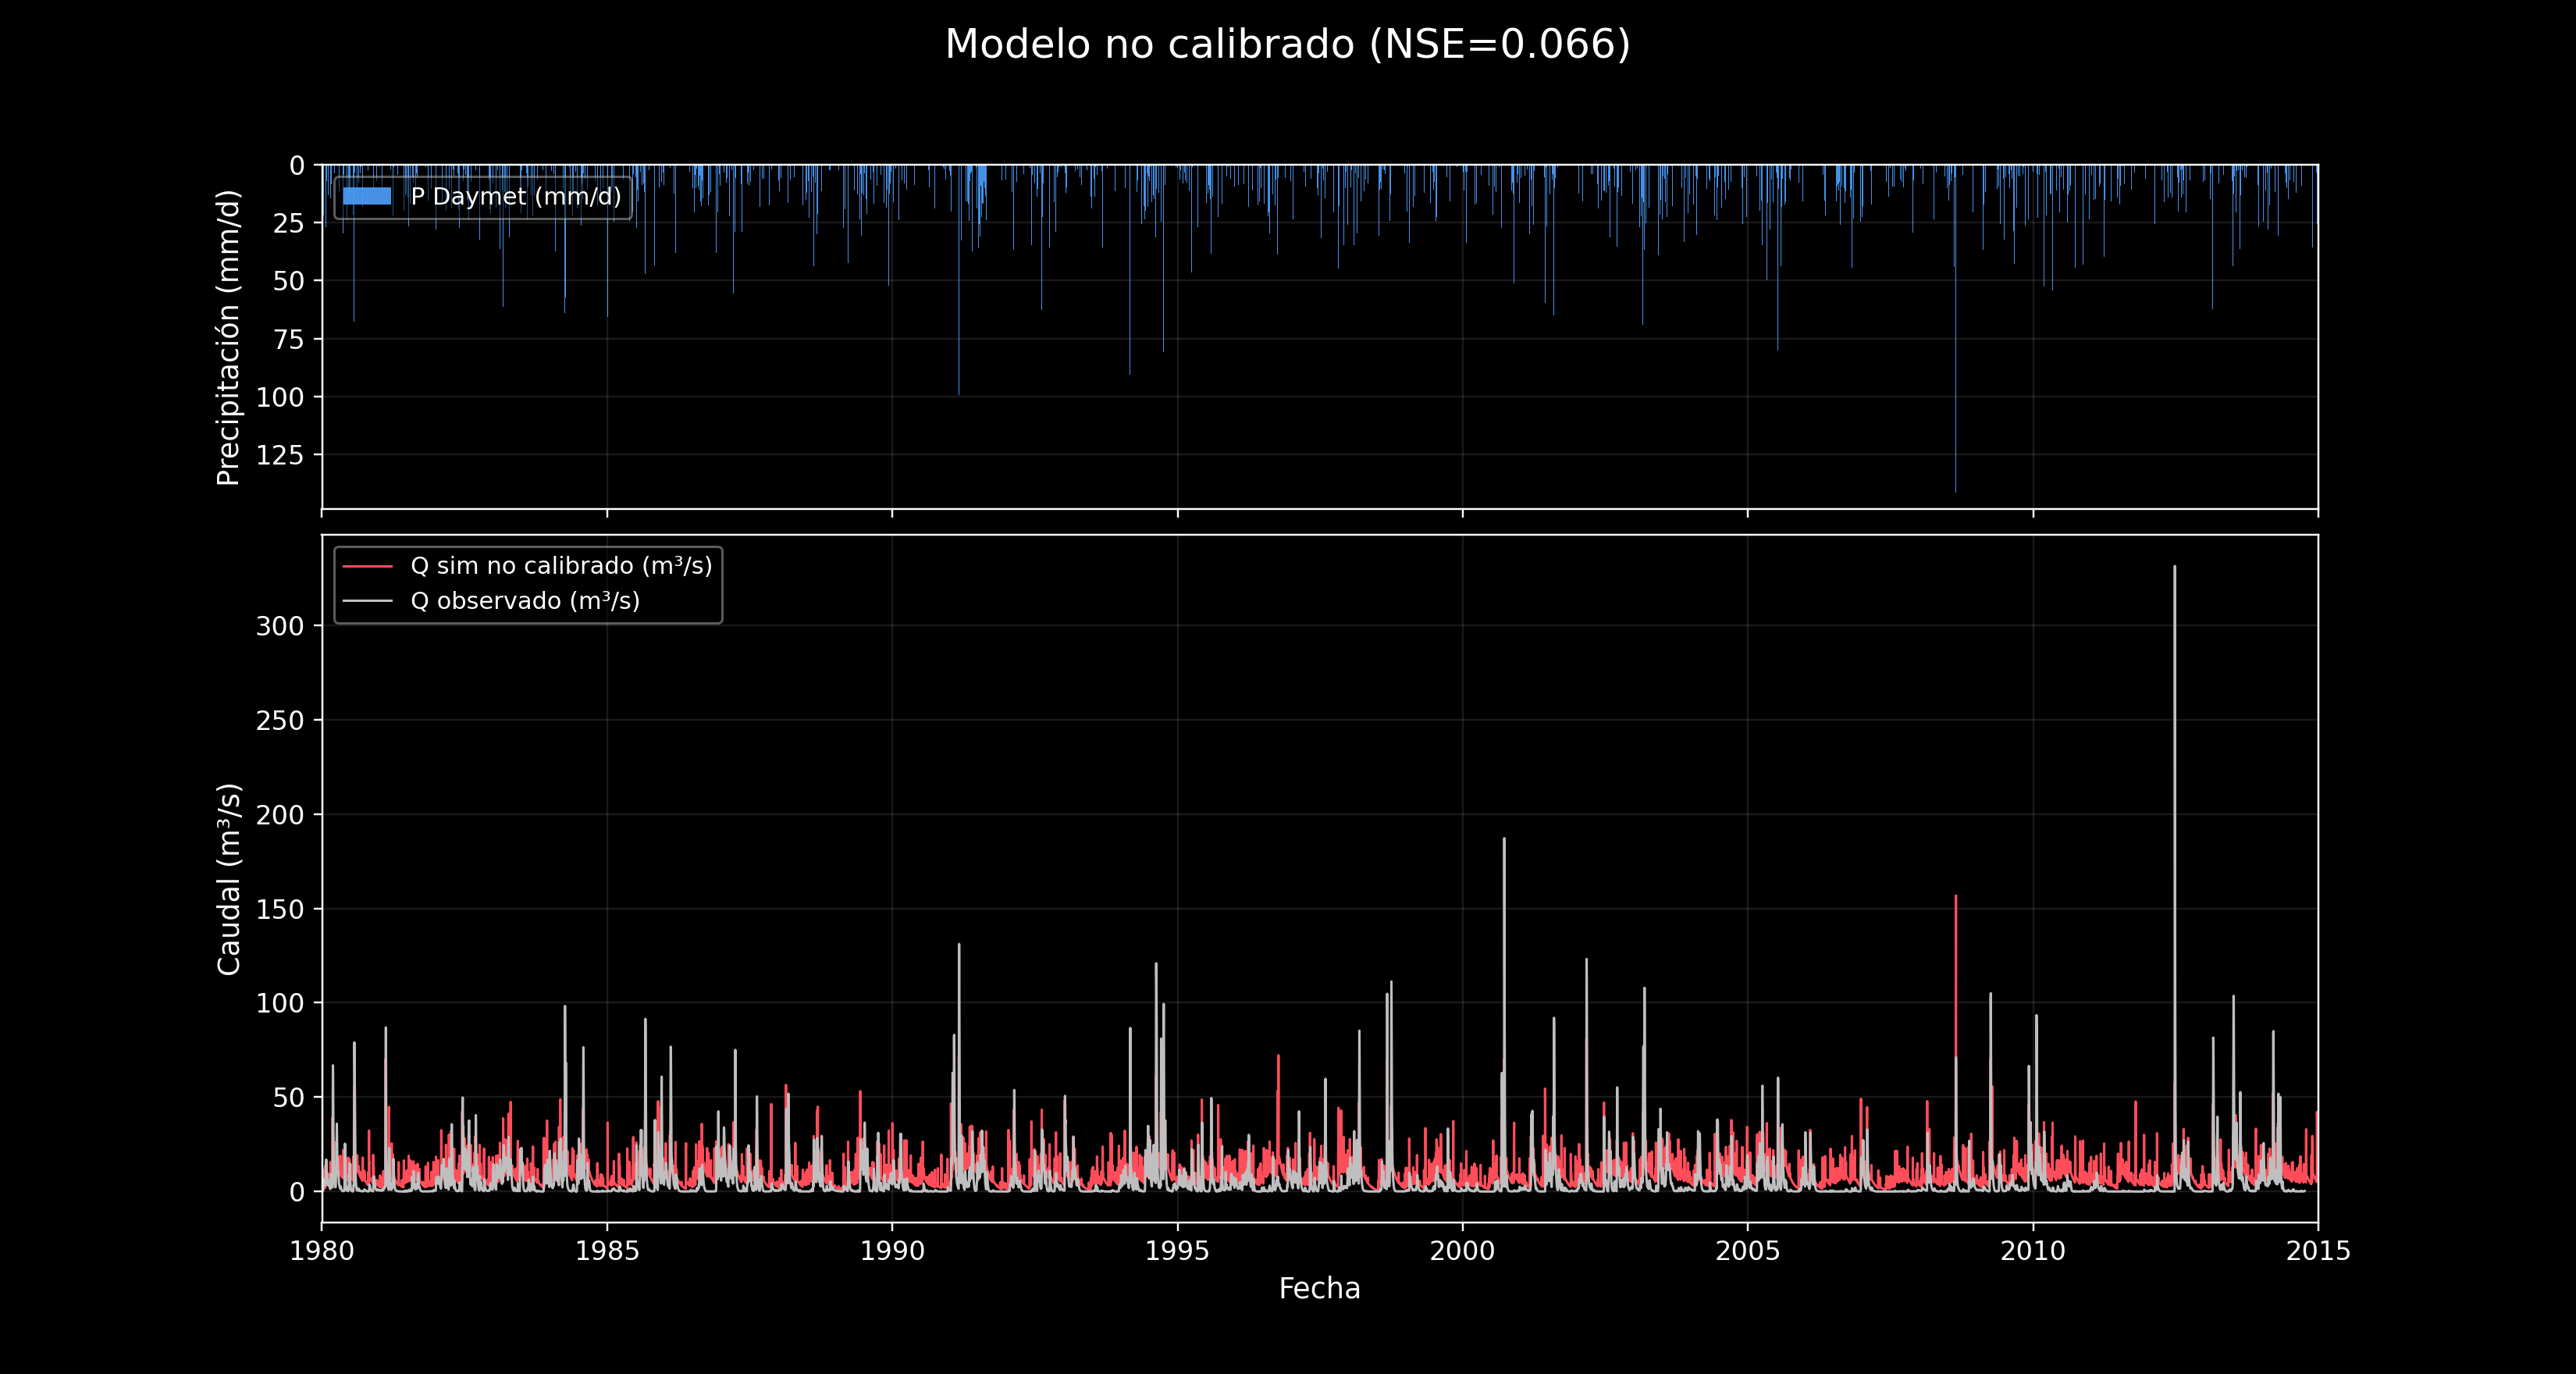
\includegraphics[width=0.95\textwidth]{../figuras/two_tank_uncalibrated_hydrograph_daymet.png}
\caption{Modelo no calibrado con Daymet.}
\end{figure}

\begin{figure}[H]
\centering
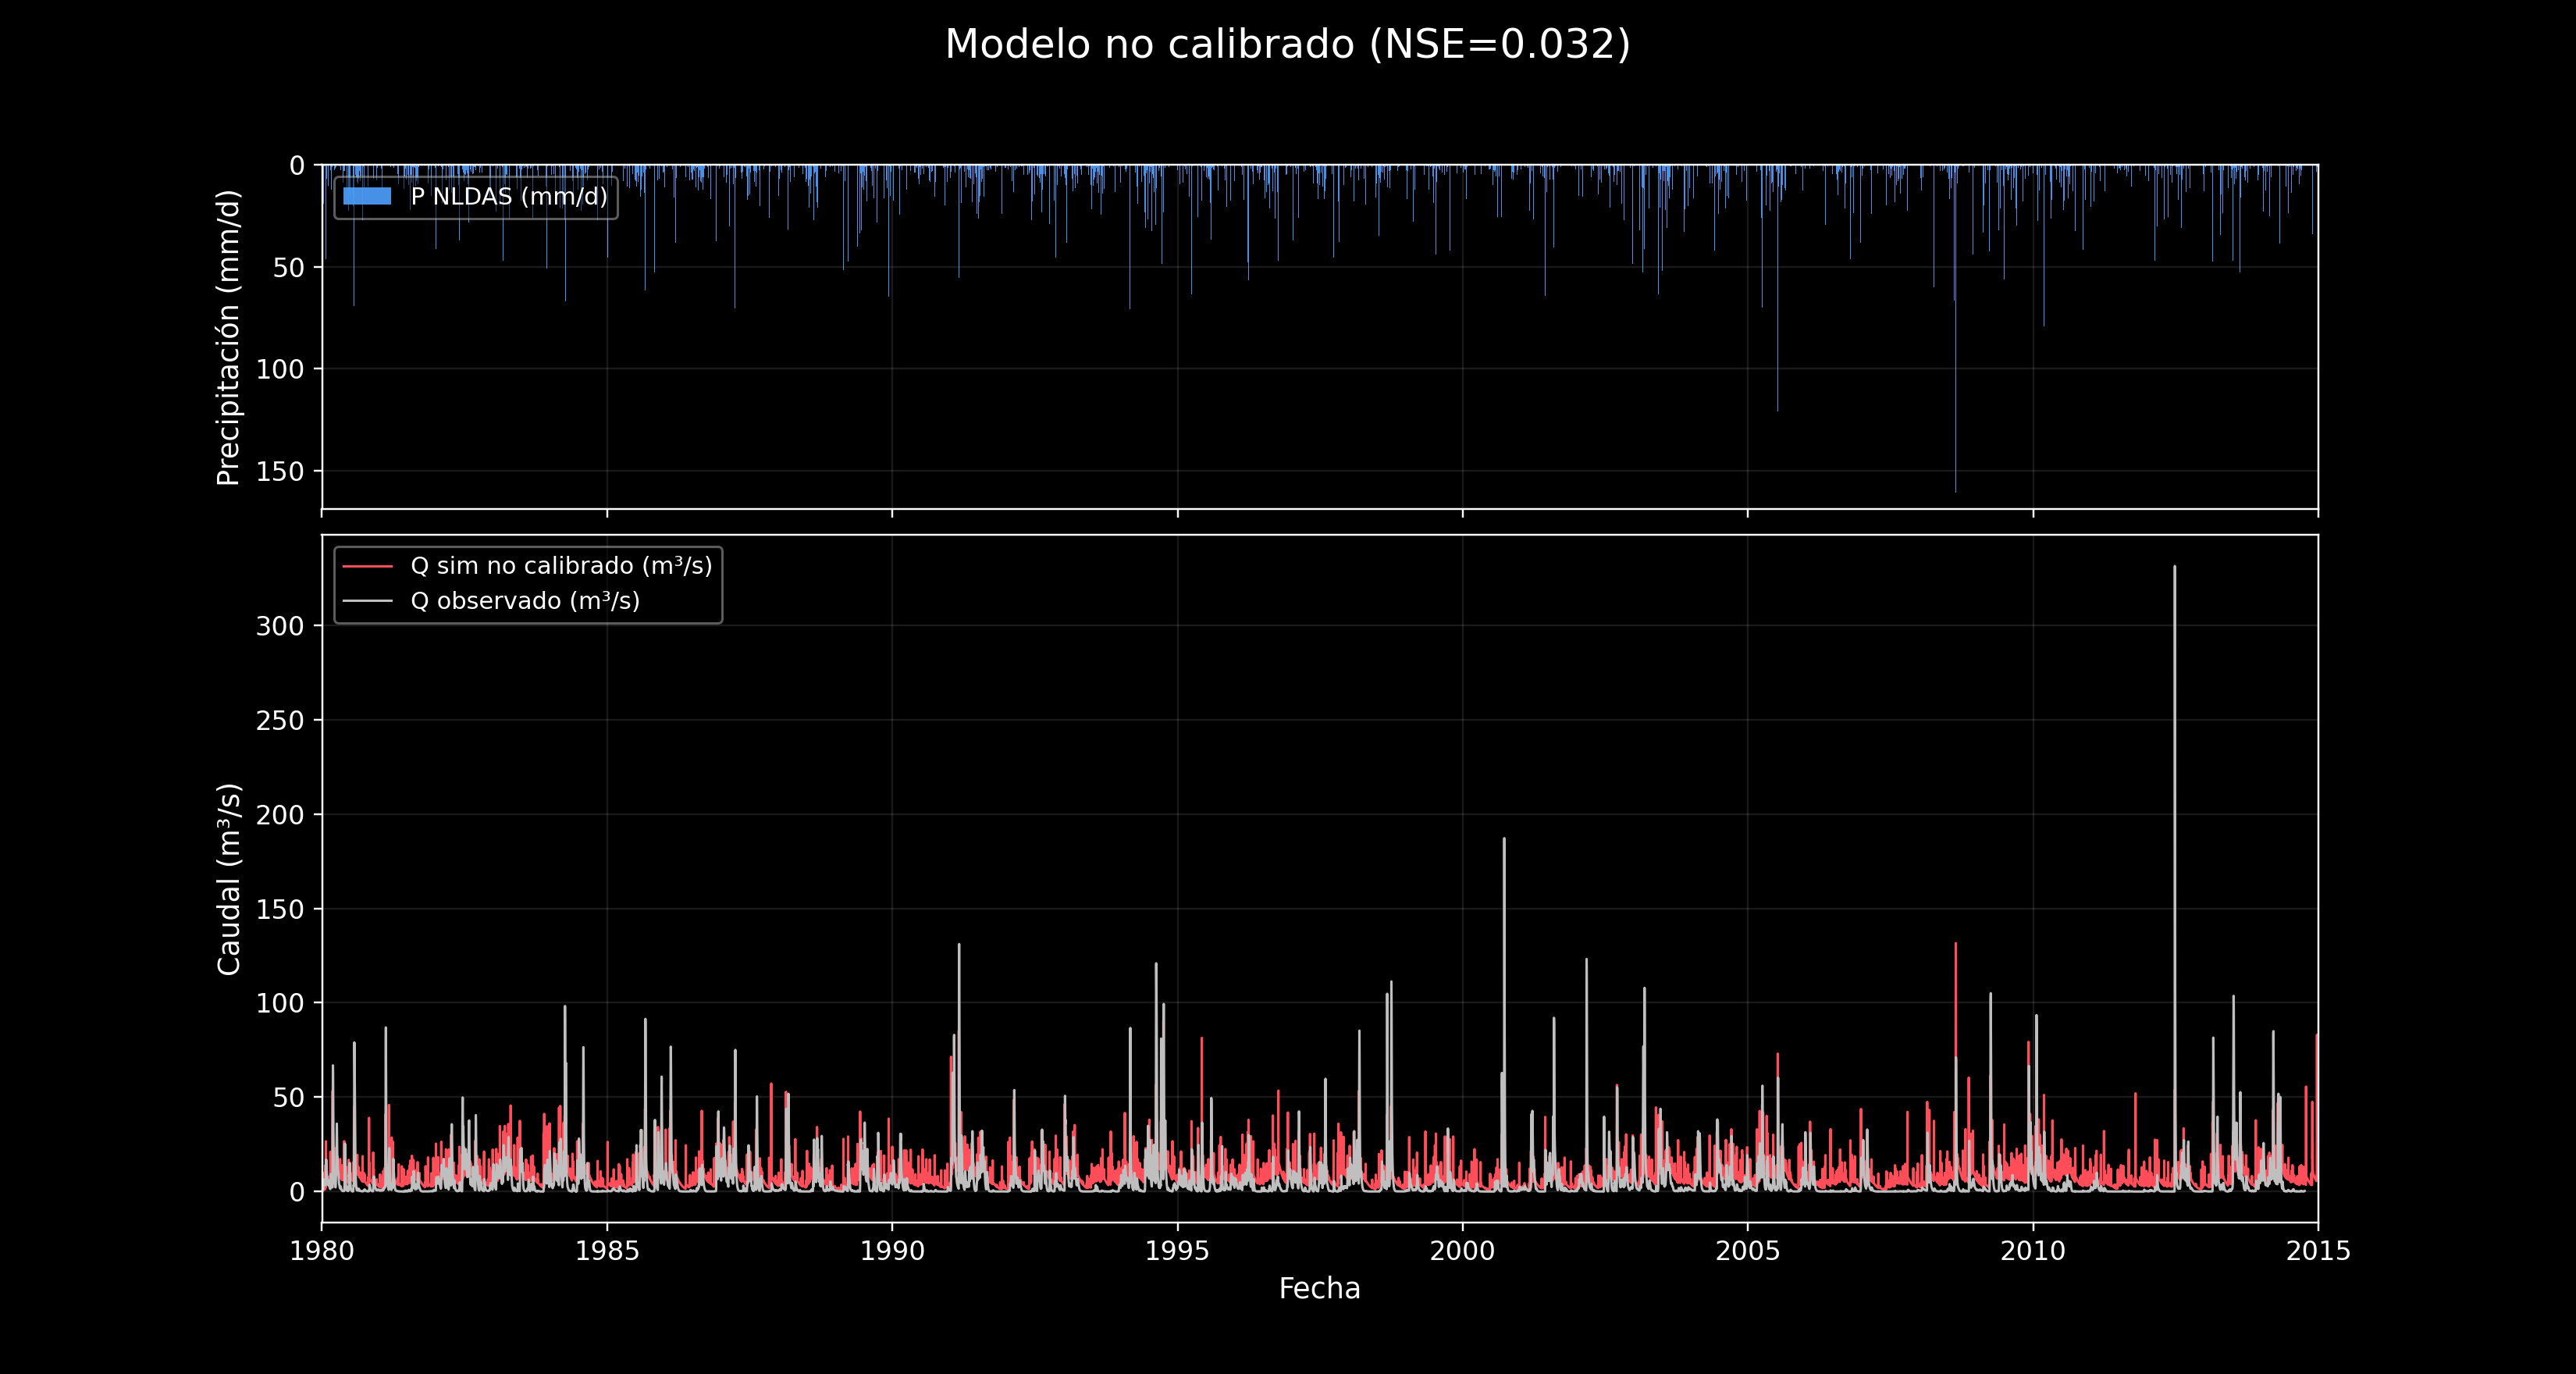
\includegraphics[width=0.95\textwidth]{../figuras/two_tank_uncalibrated_hydrograph_nldas.png}
\caption{Modelo no calibrado con NLDAS.}
\end{figure}

\textbf{Desempeno del modelo no calibrado}

Con Daymet como forzamiento, el modelo presenta un desempeno bajo (NSE = 0.066). Aunque reproduce la ocurrencia general de eventos asociados a episodios de precipitacion, se observa subestimacion sistematica de picos y una respuesta suavizada ante eventos extremos.

Con NLDAS, el desempeno es aun menor (NSE = 0.032), evidenciando mayor amortiguamiento en la respuesta hidrologica. Estas diferencias preliminares sugieren sensibilidad del modelo a la fuente de precipitacion, lo que podria influir en los parametros optimos durante la calibracion.

No obstante, el comportamiento temporal es estable y fisicamente consistente, validando la correcta implementacion estructural del modelo previo a la optimizacion de parametros.

\textbf{Consistencia de unidades en la implementacion}

El balance hidrico interno del modelo se resolvio completamente en unidades de lamina de agua (mm/dia). La precipitacion, evapotranspiracion, caudal simulado y variaciones de almacenamiento fueron expresadas en mm/dia, garantizando coherencia dimensional y conservacion de masa.

Para efectos de evaluacion del desempeno, el caudal simulado fue convertido a m$^3$/s mediante un factor de conversion estimado a partir de la relacion entre caudal observado en m$^3$/s y su equivalente en mm/dia. Este procedimiento asegura consistencia entre el sistema interno de balance y las metricas estandar utilizadas en hidrologia (NSE, KGE).

Dashboard interactivo de balance hidrico disponible en la version HTML del informe.

\textbf{Verificacion del balance hidrico}

Se evaluo la consistencia interna del modelo mediante la verificacion explicita del balance diario:
\[
P_t = ET_t + Q_t + \Delta S_t + r_t
\]

La comparacion entre la precipitacion acumulada y la suma acumulada de $(ET + Q + \Delta S)$ muestra curvas practicamente identicas durante todo el periodo 1980--2014. El residual acumulado final es del orden de $10^{-12}$ mm, valor numericamente despreciable atribuible a redondeo en punto flotante. En terminos practicos, \textbf{el cierre de masa es exacto}.

El diagrama de Sankey confirma que la particion integrada entre evapotranspiracion, escorrentia simulada y cambio neto de almacenamiento es fisicamente coherente. El heatmap del residual mensual muestra valores del orden de $10^{-14}$ mm/d sin patrones estacionales, confirmando ausencia de sesgos estructurales o errores de signo en el balance.

\subsection*{Parte 4 - Calibracion}
Se calibro el modelo conceptual de dos tanques utilizando dos algoritmos de optimizacion global: Differential Evolution (DE) y Dual Annealing (DA). La funcion objetivo fue el coeficiente de eficiencia de Nash--Sutcliffe (NSE), maximizando su valor (equivalentemente, minimizando $-NSE$).

Se aplico un periodo de warm-up de 365 dias para reducir la influencia de las condiciones iniciales. Posteriormente, se definieron dos periodos:
\begin{itemize}
\item Calibracion: 1990--1999
\item Validacion: 2000--2009
\end{itemize}

La calibracion se realizo de forma independiente para dos fuentes de precipitacion (Daymet y NLDAS), resultando en cuatro combinaciones fuente--metodo.

Las siguientes figuras muestran los hidrogramas diarios para cada combinacion fuente--metodo. El menu desplegable en el reporte interactivo permite seleccionar el algoritmo de optimizacion (DA o DE) para cada fuente de precipitacion.

\begin{figure}[H]
\centering
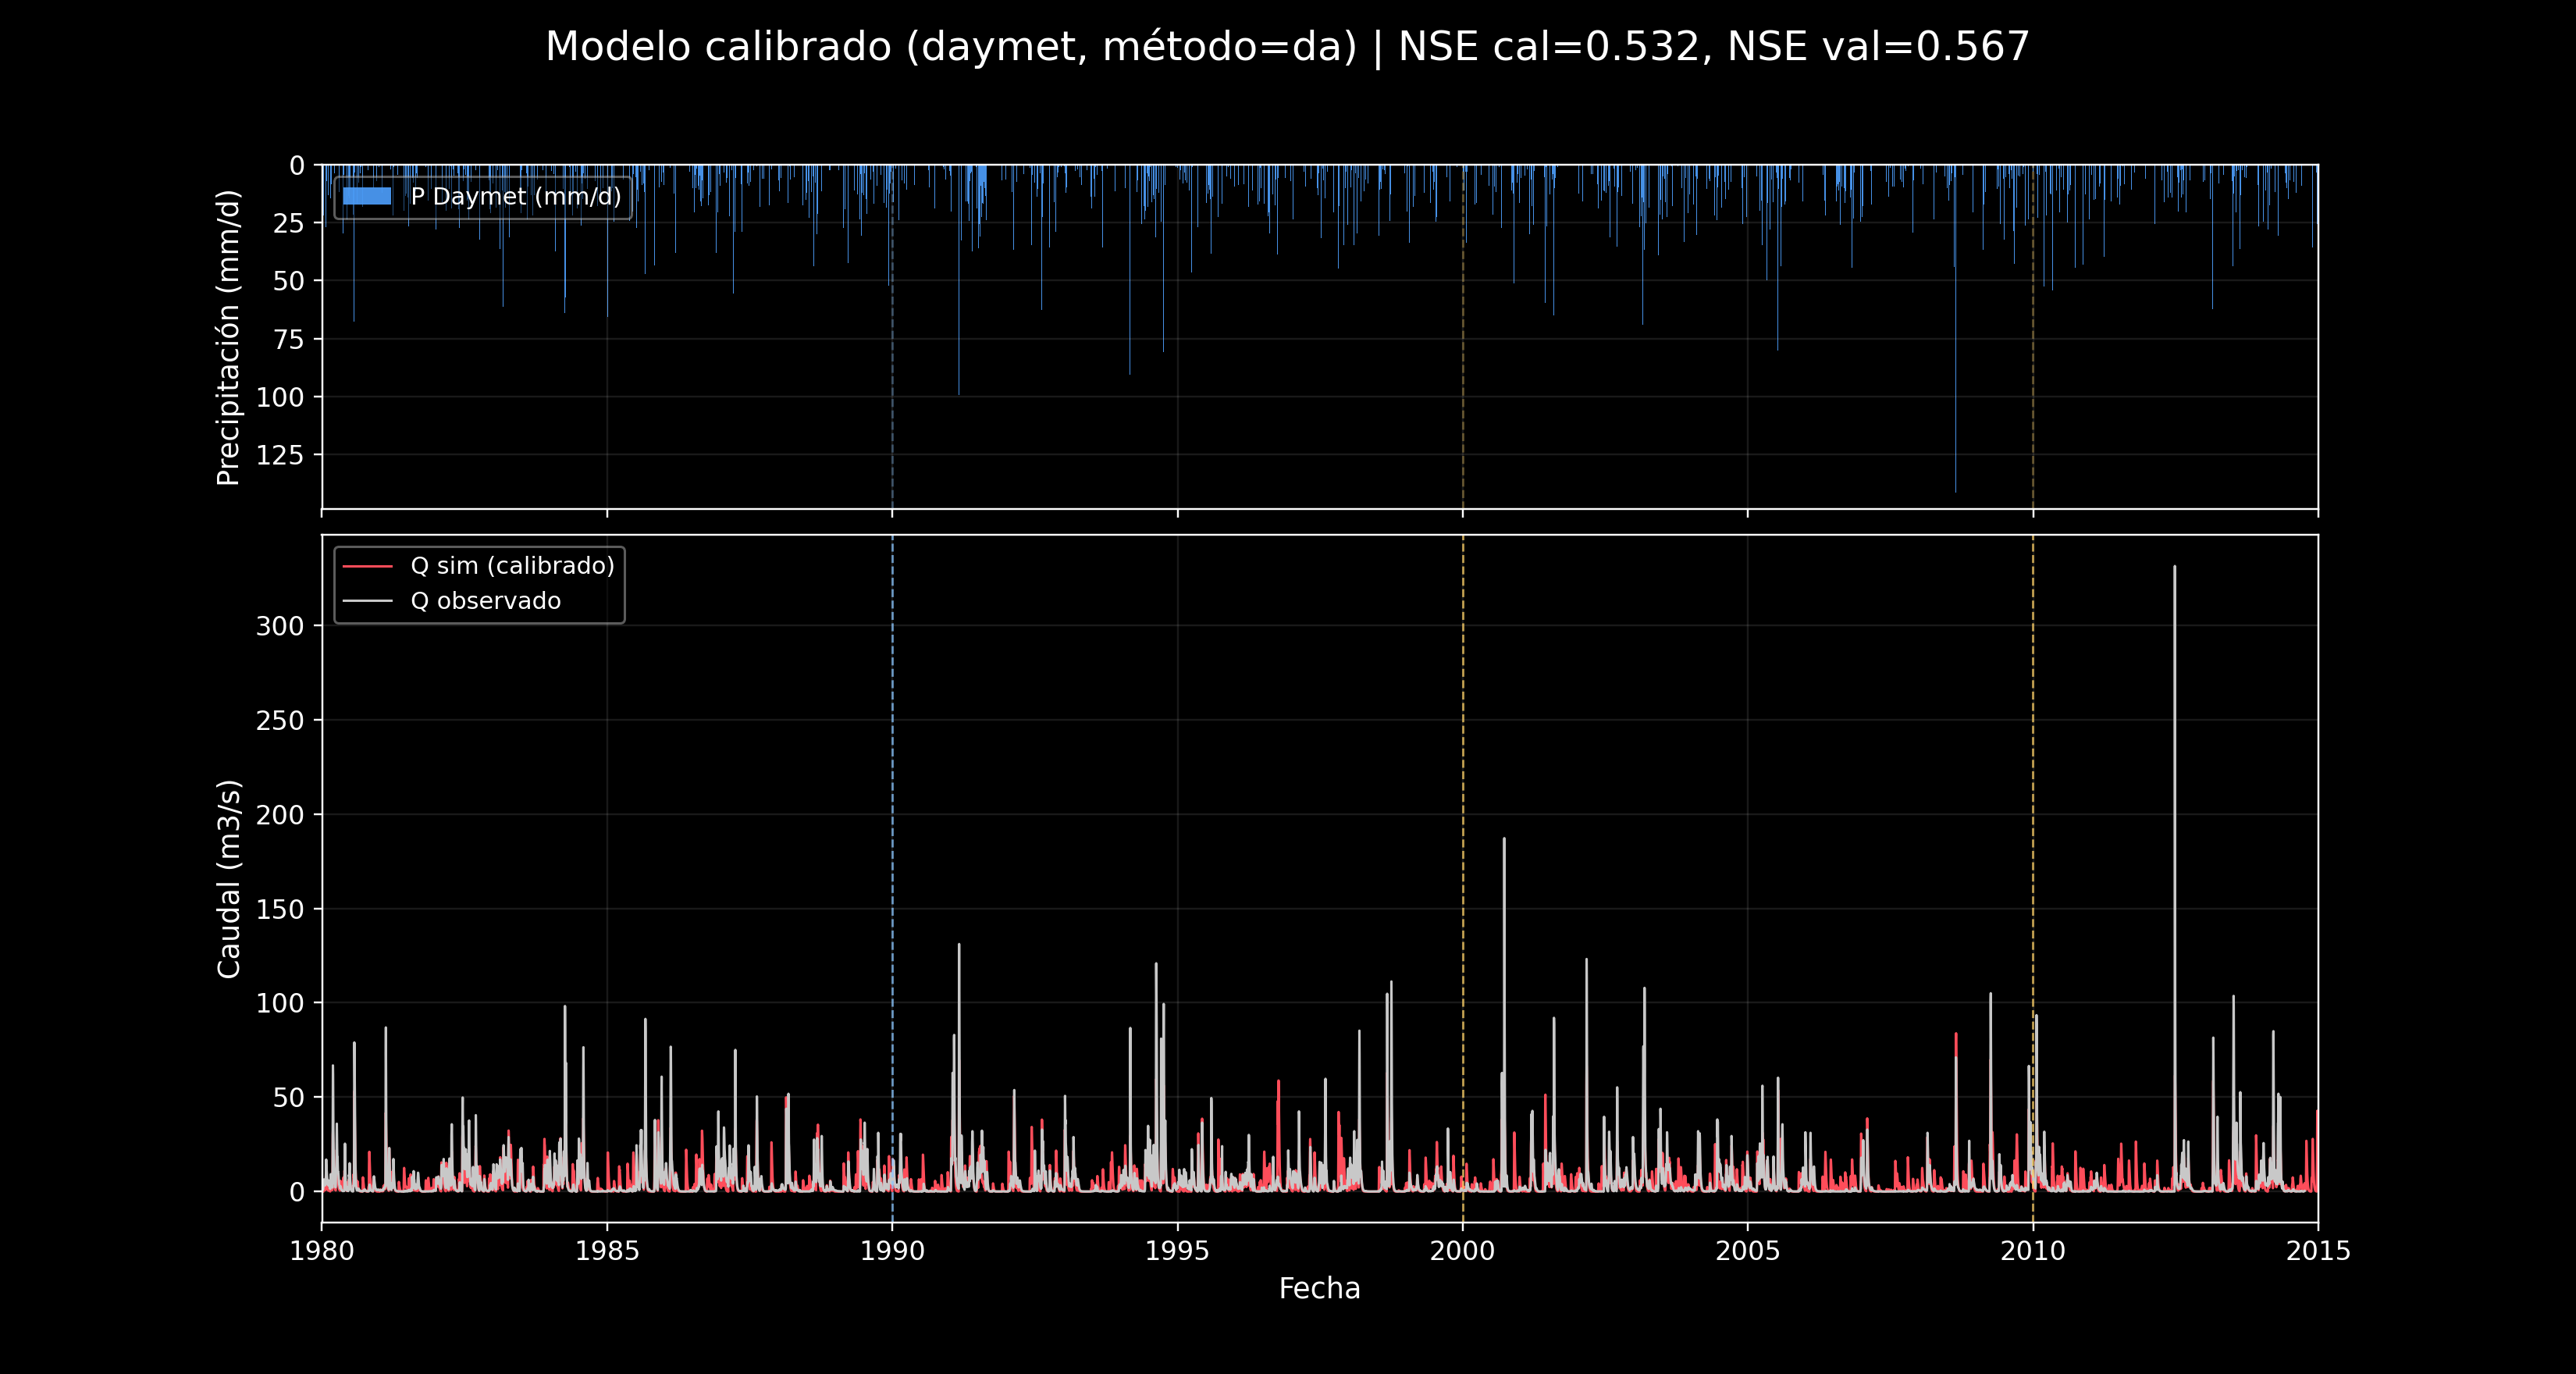
\includegraphics[width=0.48\textwidth]{../figuras/hidrograma_calibrado_daymet_da.png}
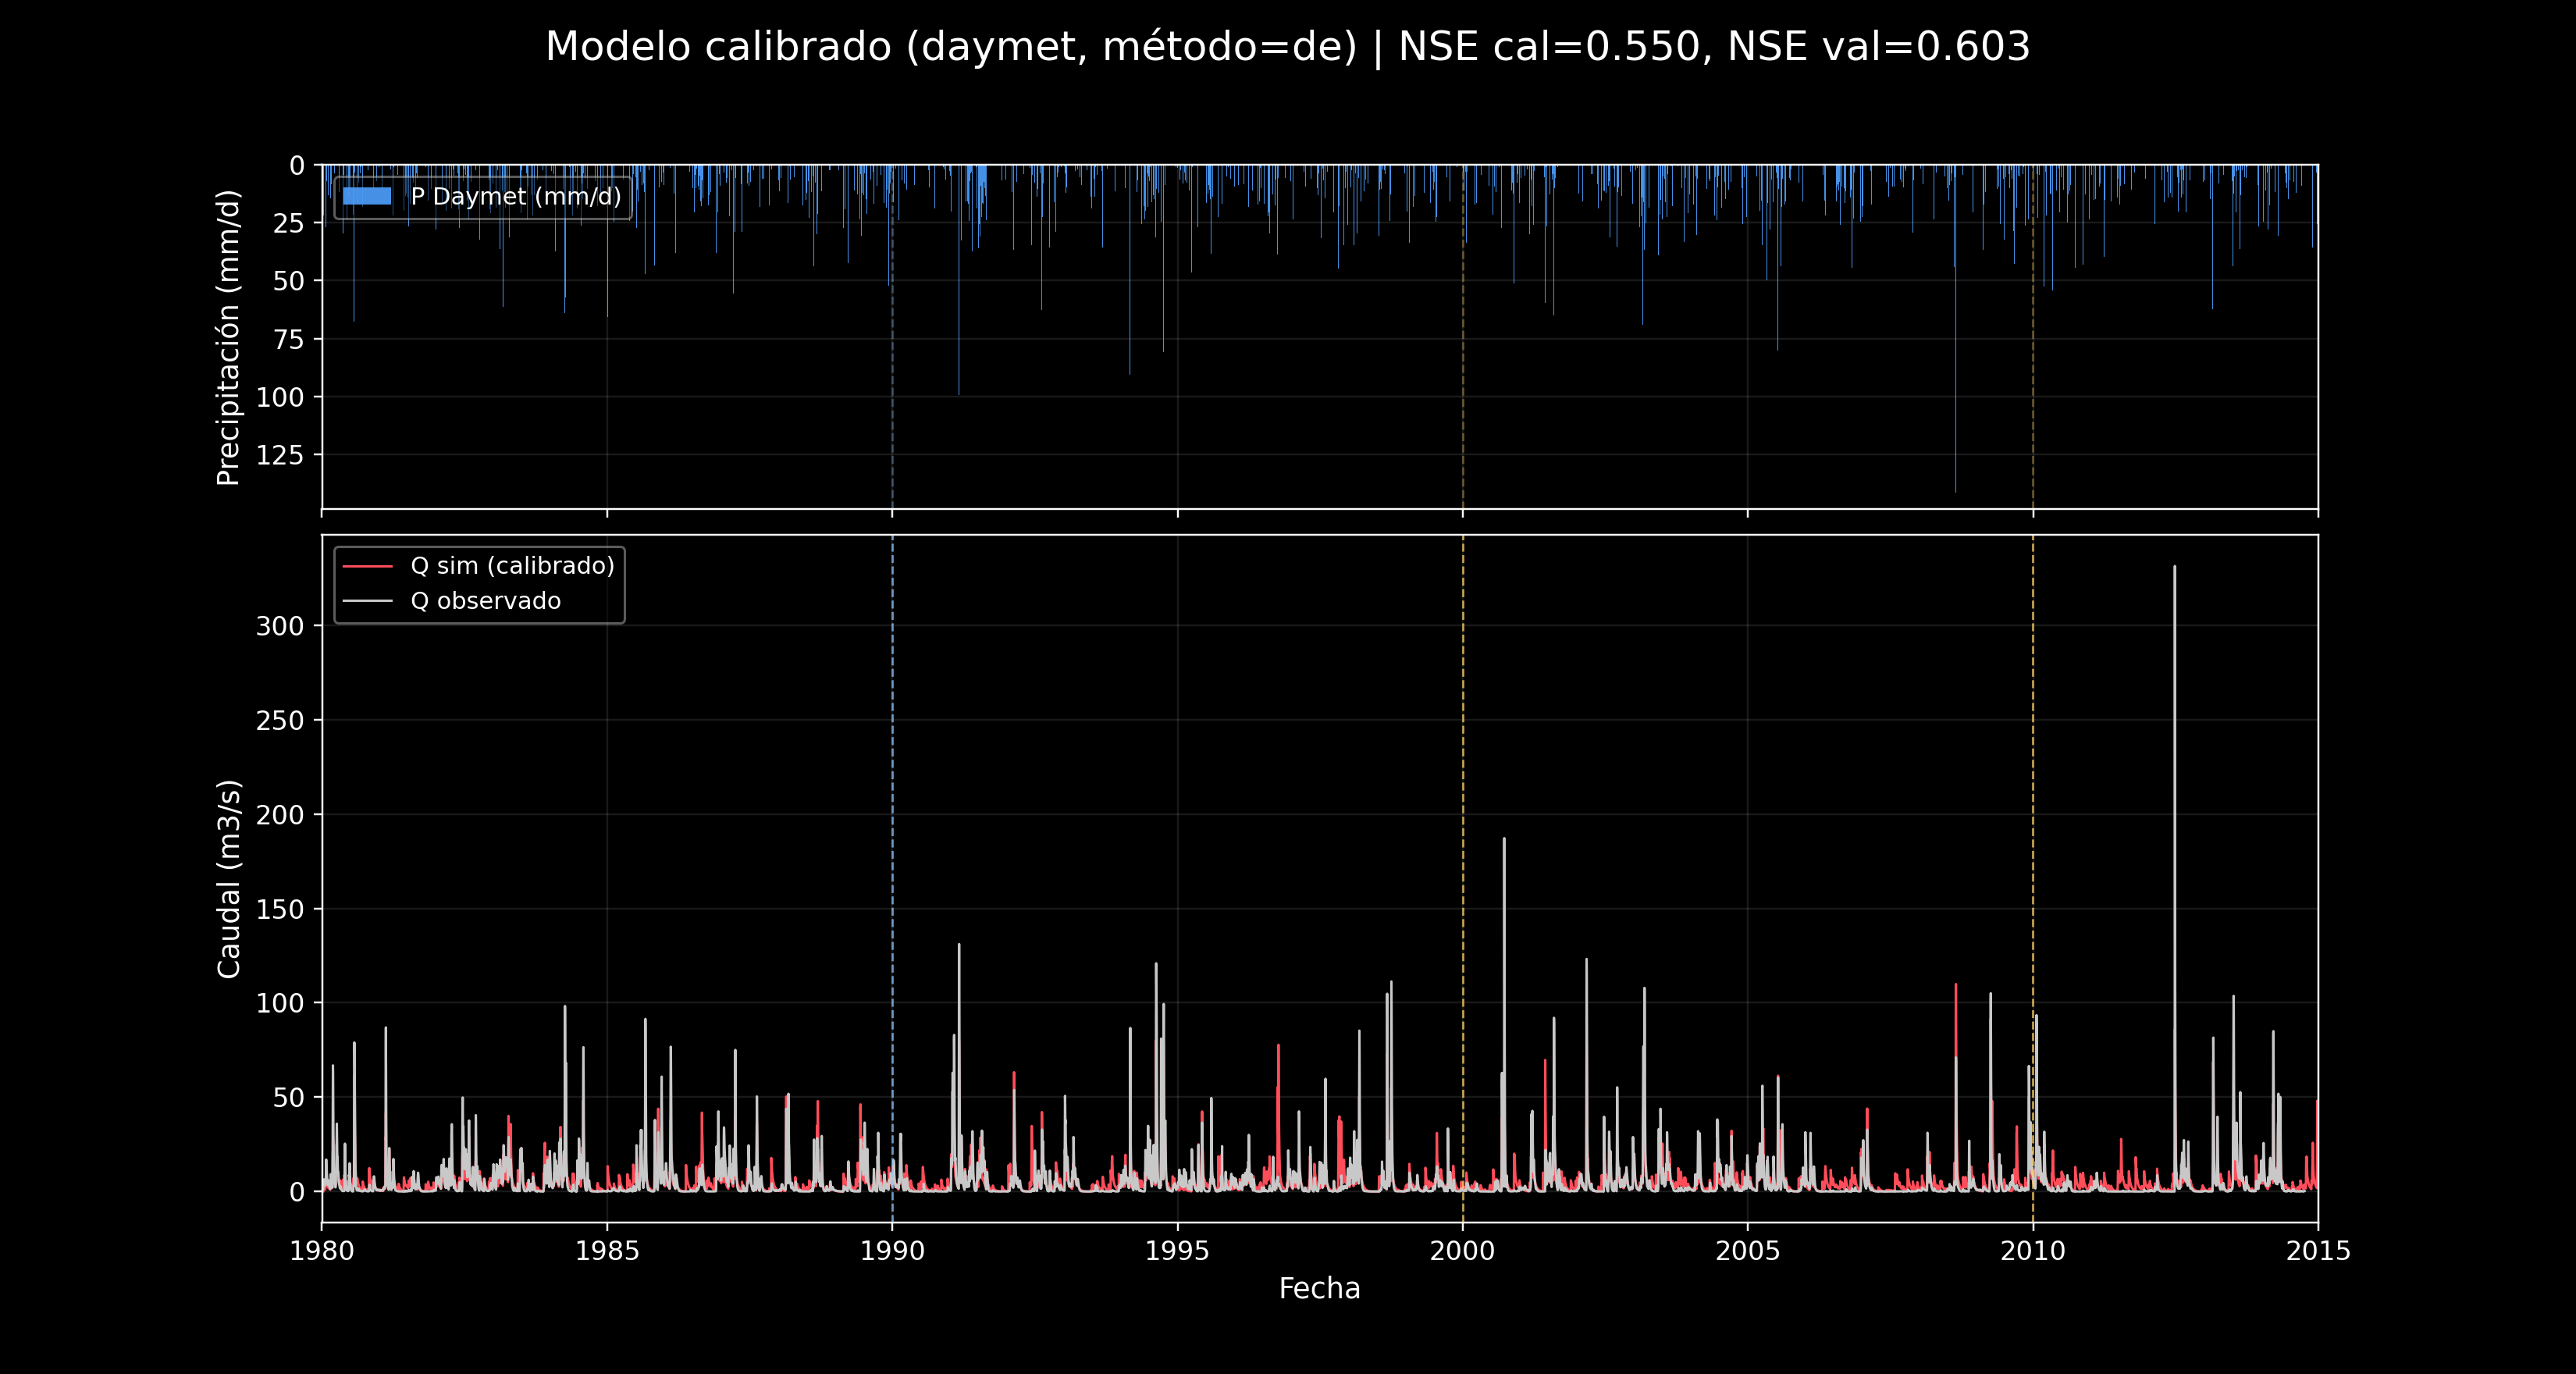
\includegraphics[width=0.48\textwidth]{../figuras/hidrograma_calibrado_daymet_de.png}
\caption{Calibrado estandar con Daymet (DA/DE).}
\end{figure}

\textbf{Desempeno con Daymet}

Para Daymet, ambos metodos produjeron ajustes satisfactorios, con una mejora de DE frente a DA:
\begin{itemize}
\item DA: NSE\_cal $\approx 0.532$; NSE\_val $\approx 0.567$
\item DE: NSE\_cal $\approx 0.550$; NSE\_val $\approx 0.603$
\end{itemize}
Esto indica un ajuste satisfactorio durante calibracion y una buena capacidad de generalizacion en validacion. Visualmente, el modelo reproduce adecuadamente la dinamica general del hidrograma, aunque persiste una ligera subestimacion en algunos picos de crecida.

\begin{figure}[H]
\centering
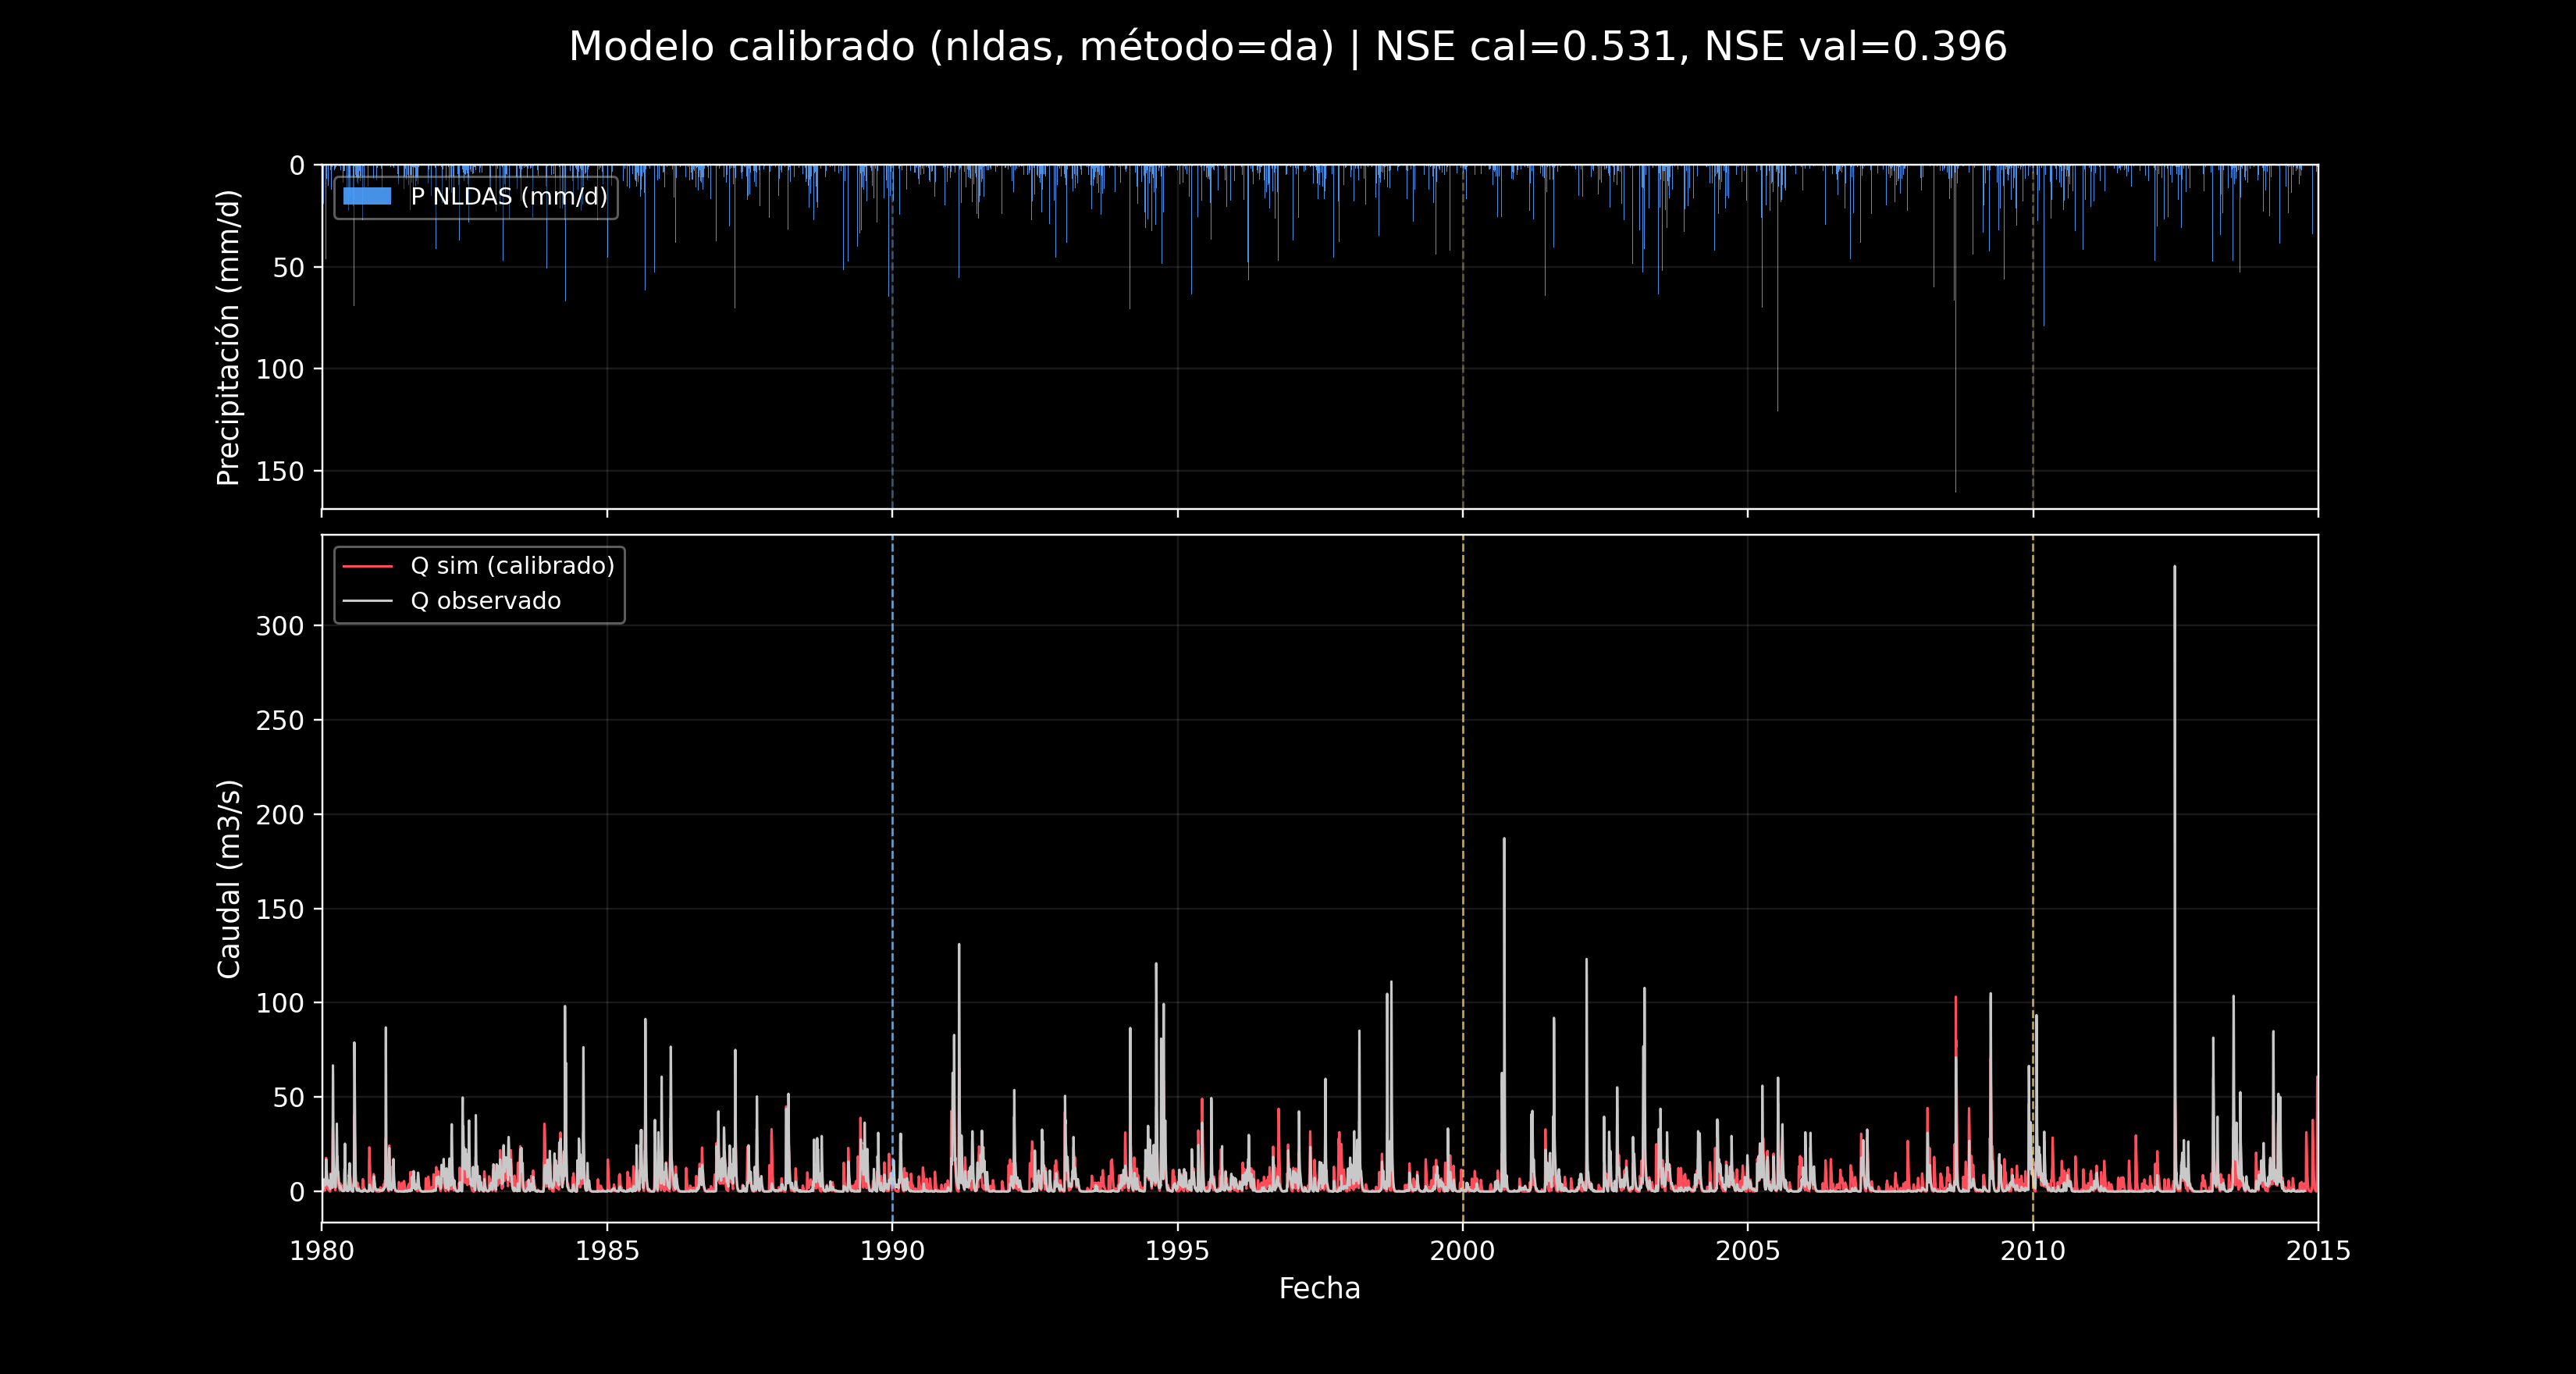
\includegraphics[width=0.48\textwidth]{../figuras/hidrograma_calibrado_nldas_da.png}
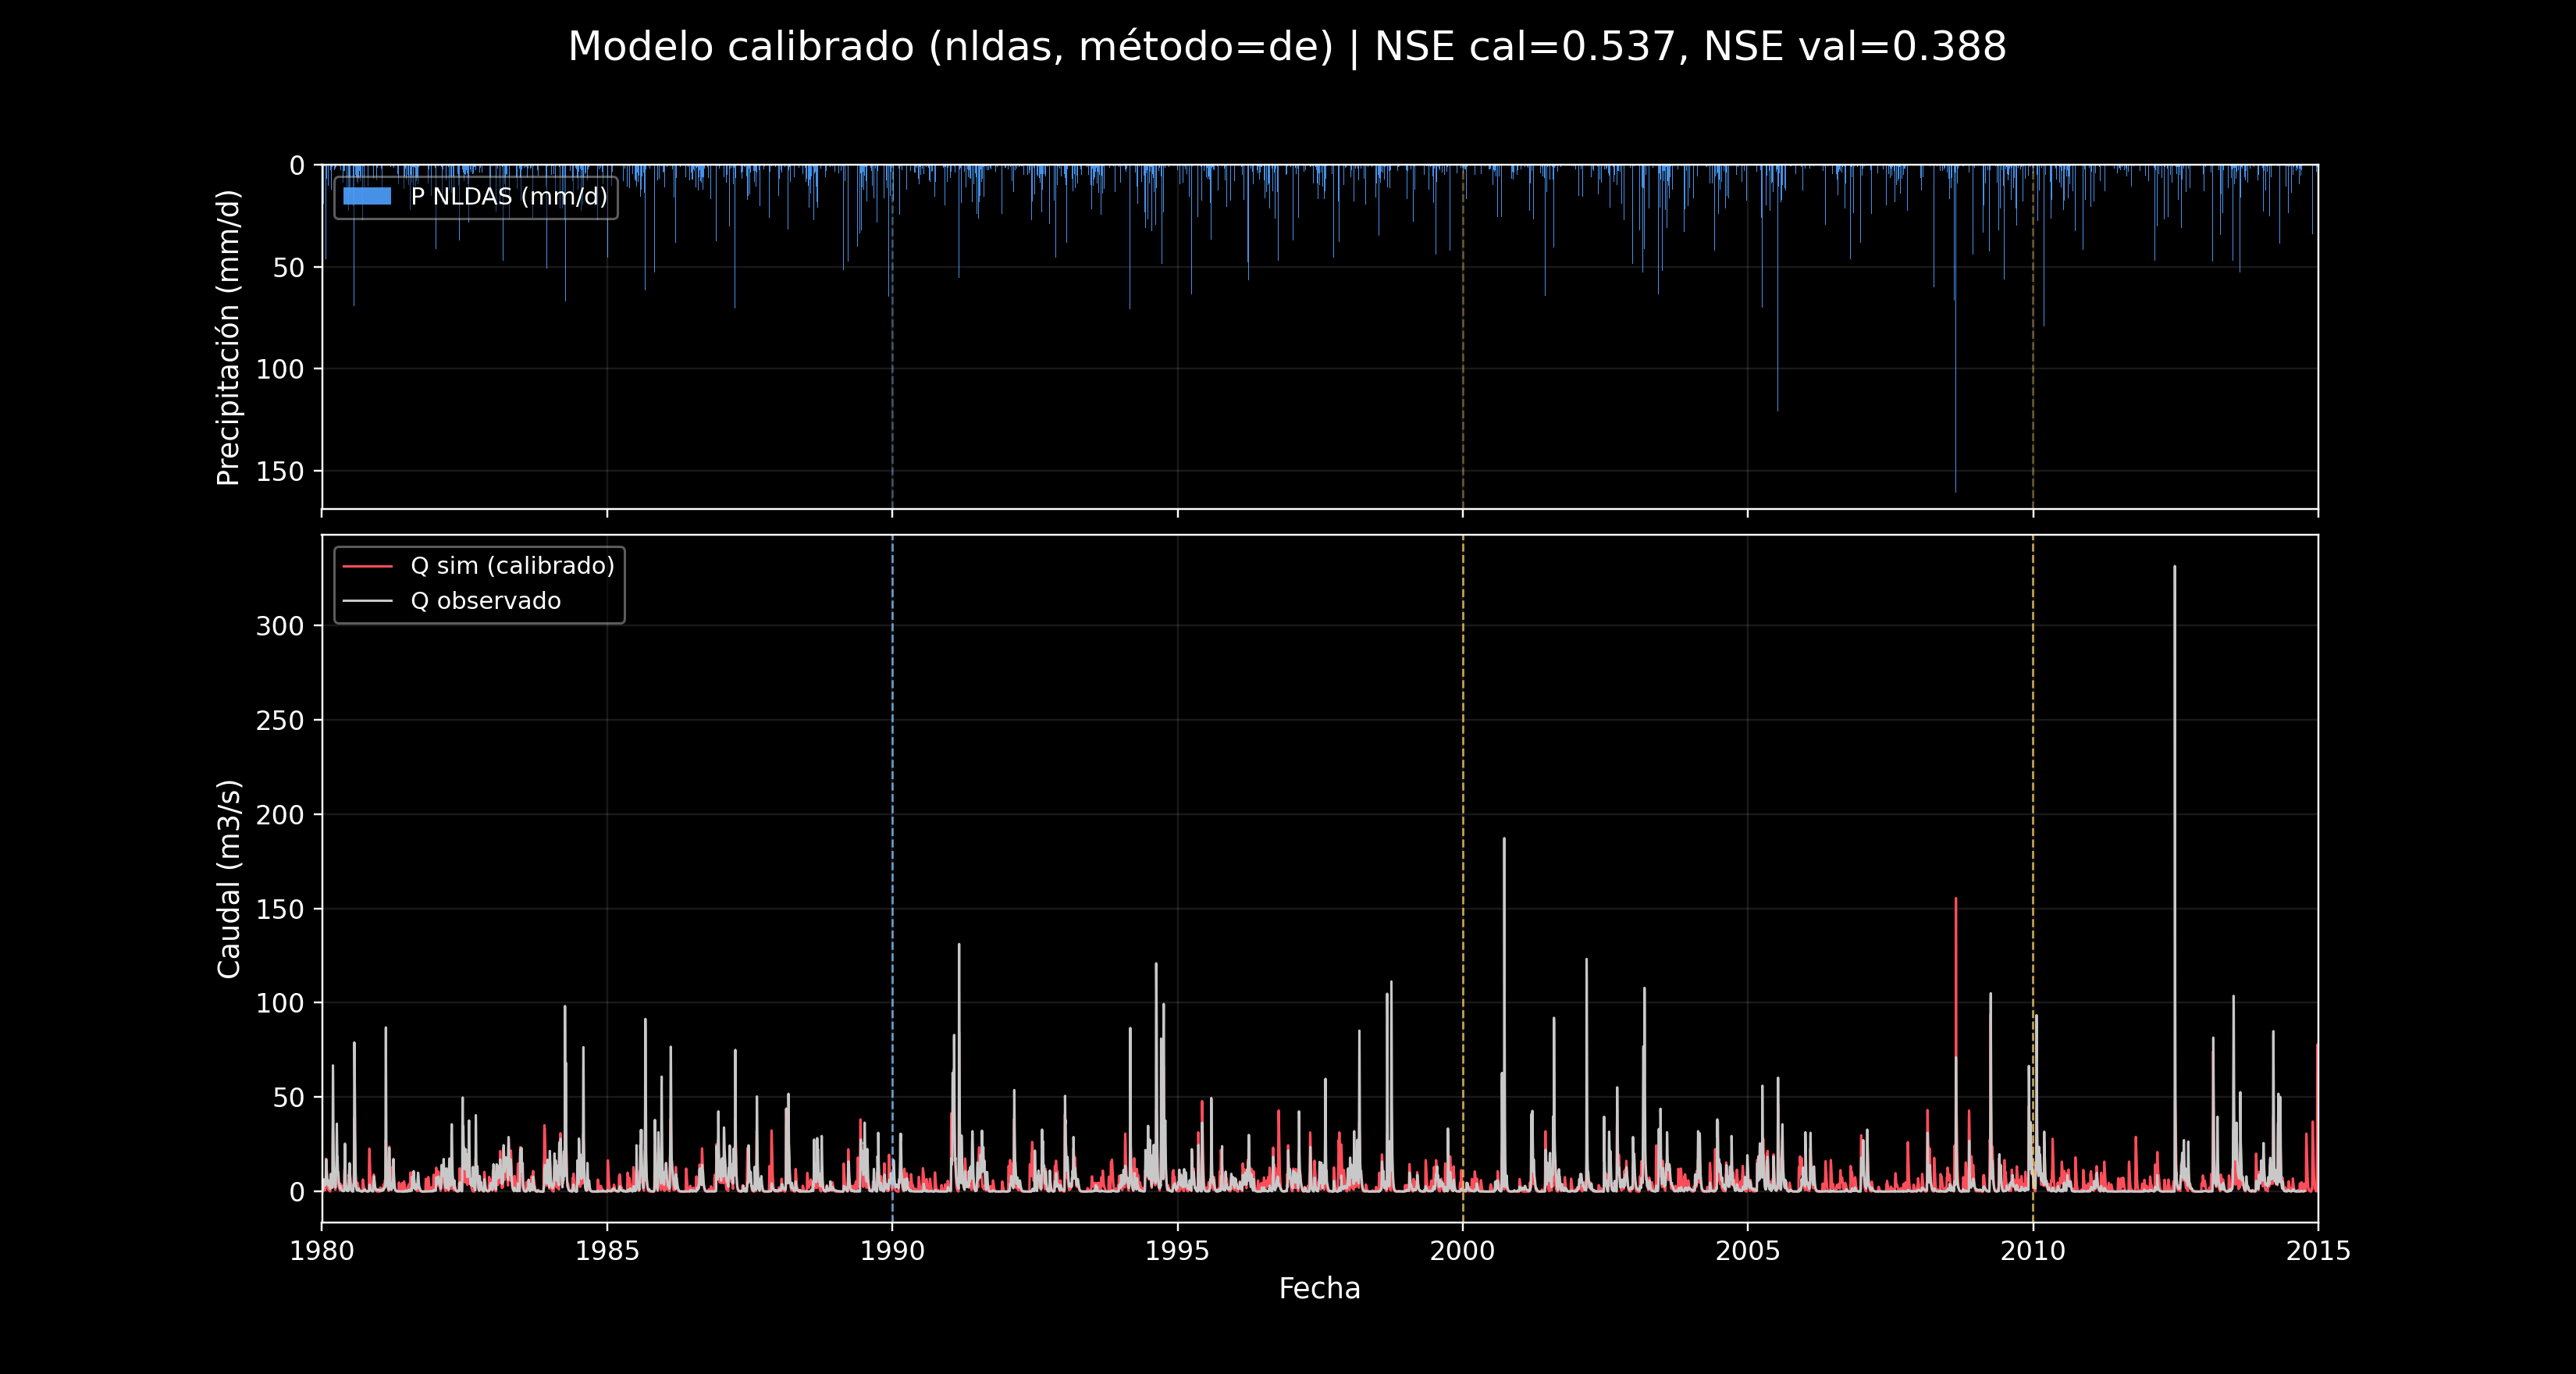
\includegraphics[width=0.48\textwidth]{../figuras/hidrograma_calibrado_nldas_de.png}
\caption{Calibrado estandar con NLDAS (DA/DE).}
\end{figure}

\textbf{Desempeno con NLDAS}

Con NLDAS se obtuvo un desempeno similar durante calibracion (NSE\_cal $\approx$ 0.531--0.537), pero una reduccion marcada en validacion (NSE\_val $\approx$ 0.389--0.397).

Esto sugiere que, para esta cuenca, la serie Daymet proporciona forzantes mas consistentes con la respuesta hidrologica observada y mayor robustez fuera del periodo calibrado.

\begin{table}[H]
        \centering
        \scriptsize
        \caption{Resultados calibración estándar (NSE)}
        \label{tab:cal_std}
        \resizebox{\textwidth}{!}{%
        \begin{tabular}{lllllllllllllll}
\toprule
Fuente & Metodo & NSE\_cal & NSE\_val & KGE\_val & PeakRatio\_val & P95Ratio\_val & ETc & beta & alpha1 & D1 & k1 & alpha2 & D2 & k2 \\
\midrule
daymet & da & 0.532 & 0.567 & 0.644 & 0.448 & 0.998 & 8.833 & 0.170 & 0.000 & 138.397 & 0.467 & 0.000 & 508.498 & 0.230 \\
daymet & de & 0.550 & 0.603 & 0.616 & 0.587 & 0.865 & 9.920 & 0.087 & 0.000 & 262.214 & 0.200 & 0.385 & 25.956 & 0.065 \\
nldas & da & 0.531 & 0.396 & 0.536 & 0.551 & 0.924 & 7.423 & 0.143 & 0.000 & 138.397 & 0.300 & 0.000 & 508.498 & 0.300 \\
nldas & de & 0.537 & 0.388 & 0.544 & 0.831 & 0.917 & 7.658 & 0.127 & 0.000 & 323.882 & 0.340 & 0.000 & 65.645 & 0.250 \\
\bottomrule
\end{tabular}

        }
        \end{table}

\textbf{Interpretacion de parametros}

Las soluciones optimas conservan $\alpha_1$ en la frontera inferior, pero muestran estructuras internas distintas entre metodos, especialmente para Daymet.

En tres de las cuatro soluciones $\alpha_2$ tambien es cercano a cero, por lo que predomina la respuesta controlada por almacenamiento y drenaje lento. Daymet--DE constituye la excepcion ($\alpha_2 \approx 0.385$ y $D_2$ mas bajo), lo que introduce una contribucion rapida y mejora el NSE de validacion.

Diferentes combinaciones parametricas producen desempenos competitivos, lo cual evidencia equifinalidad bajo un criterio basado unicamente en NSE.

\textbf{\large En conjunto, la calibracion estandar indica que Daymet--DE ofrece el mejor desempeno global, al alcanzar el mayor NSE en validacion (0.603). La ventaja de Daymet frente a NLDAS es mayor que la diferencia entre optimizadores.}


\vspace{0.5em}
{\Large\textbf{\textcolor{cyan}{Analisis complementario enfocado en crecidas}}}

\textbf{Calibracion orientada a extremos (objetivo: $J$)}

Adicionalmente, se realizo una calibracion enfocada en la representacion de eventos de crecida mediante una funcion objetivo compuesta $J$, que prioriza la reproduccion de altos caudales e incorpora penalizacion por subestimacion de picos.

Se mantuvieron las mismas configuraciones de optimizacion (DE y DA), periodos de calibracion (1990--1999) y validacion (2000--2009), asi como el warm-up de 365 dias. La calibracion se ejecuto nuevamente para Daymet y NLDAS, resultando en cuatro combinaciones fuente--metodo.

Las figuras siguientes muestran los hidrogramas correspondientes; en el reporte interactivo el menu desplegable permite seleccionar el algoritmo (DA o DE) para cada fuente.


        

\begin{figure}[H]
\centering
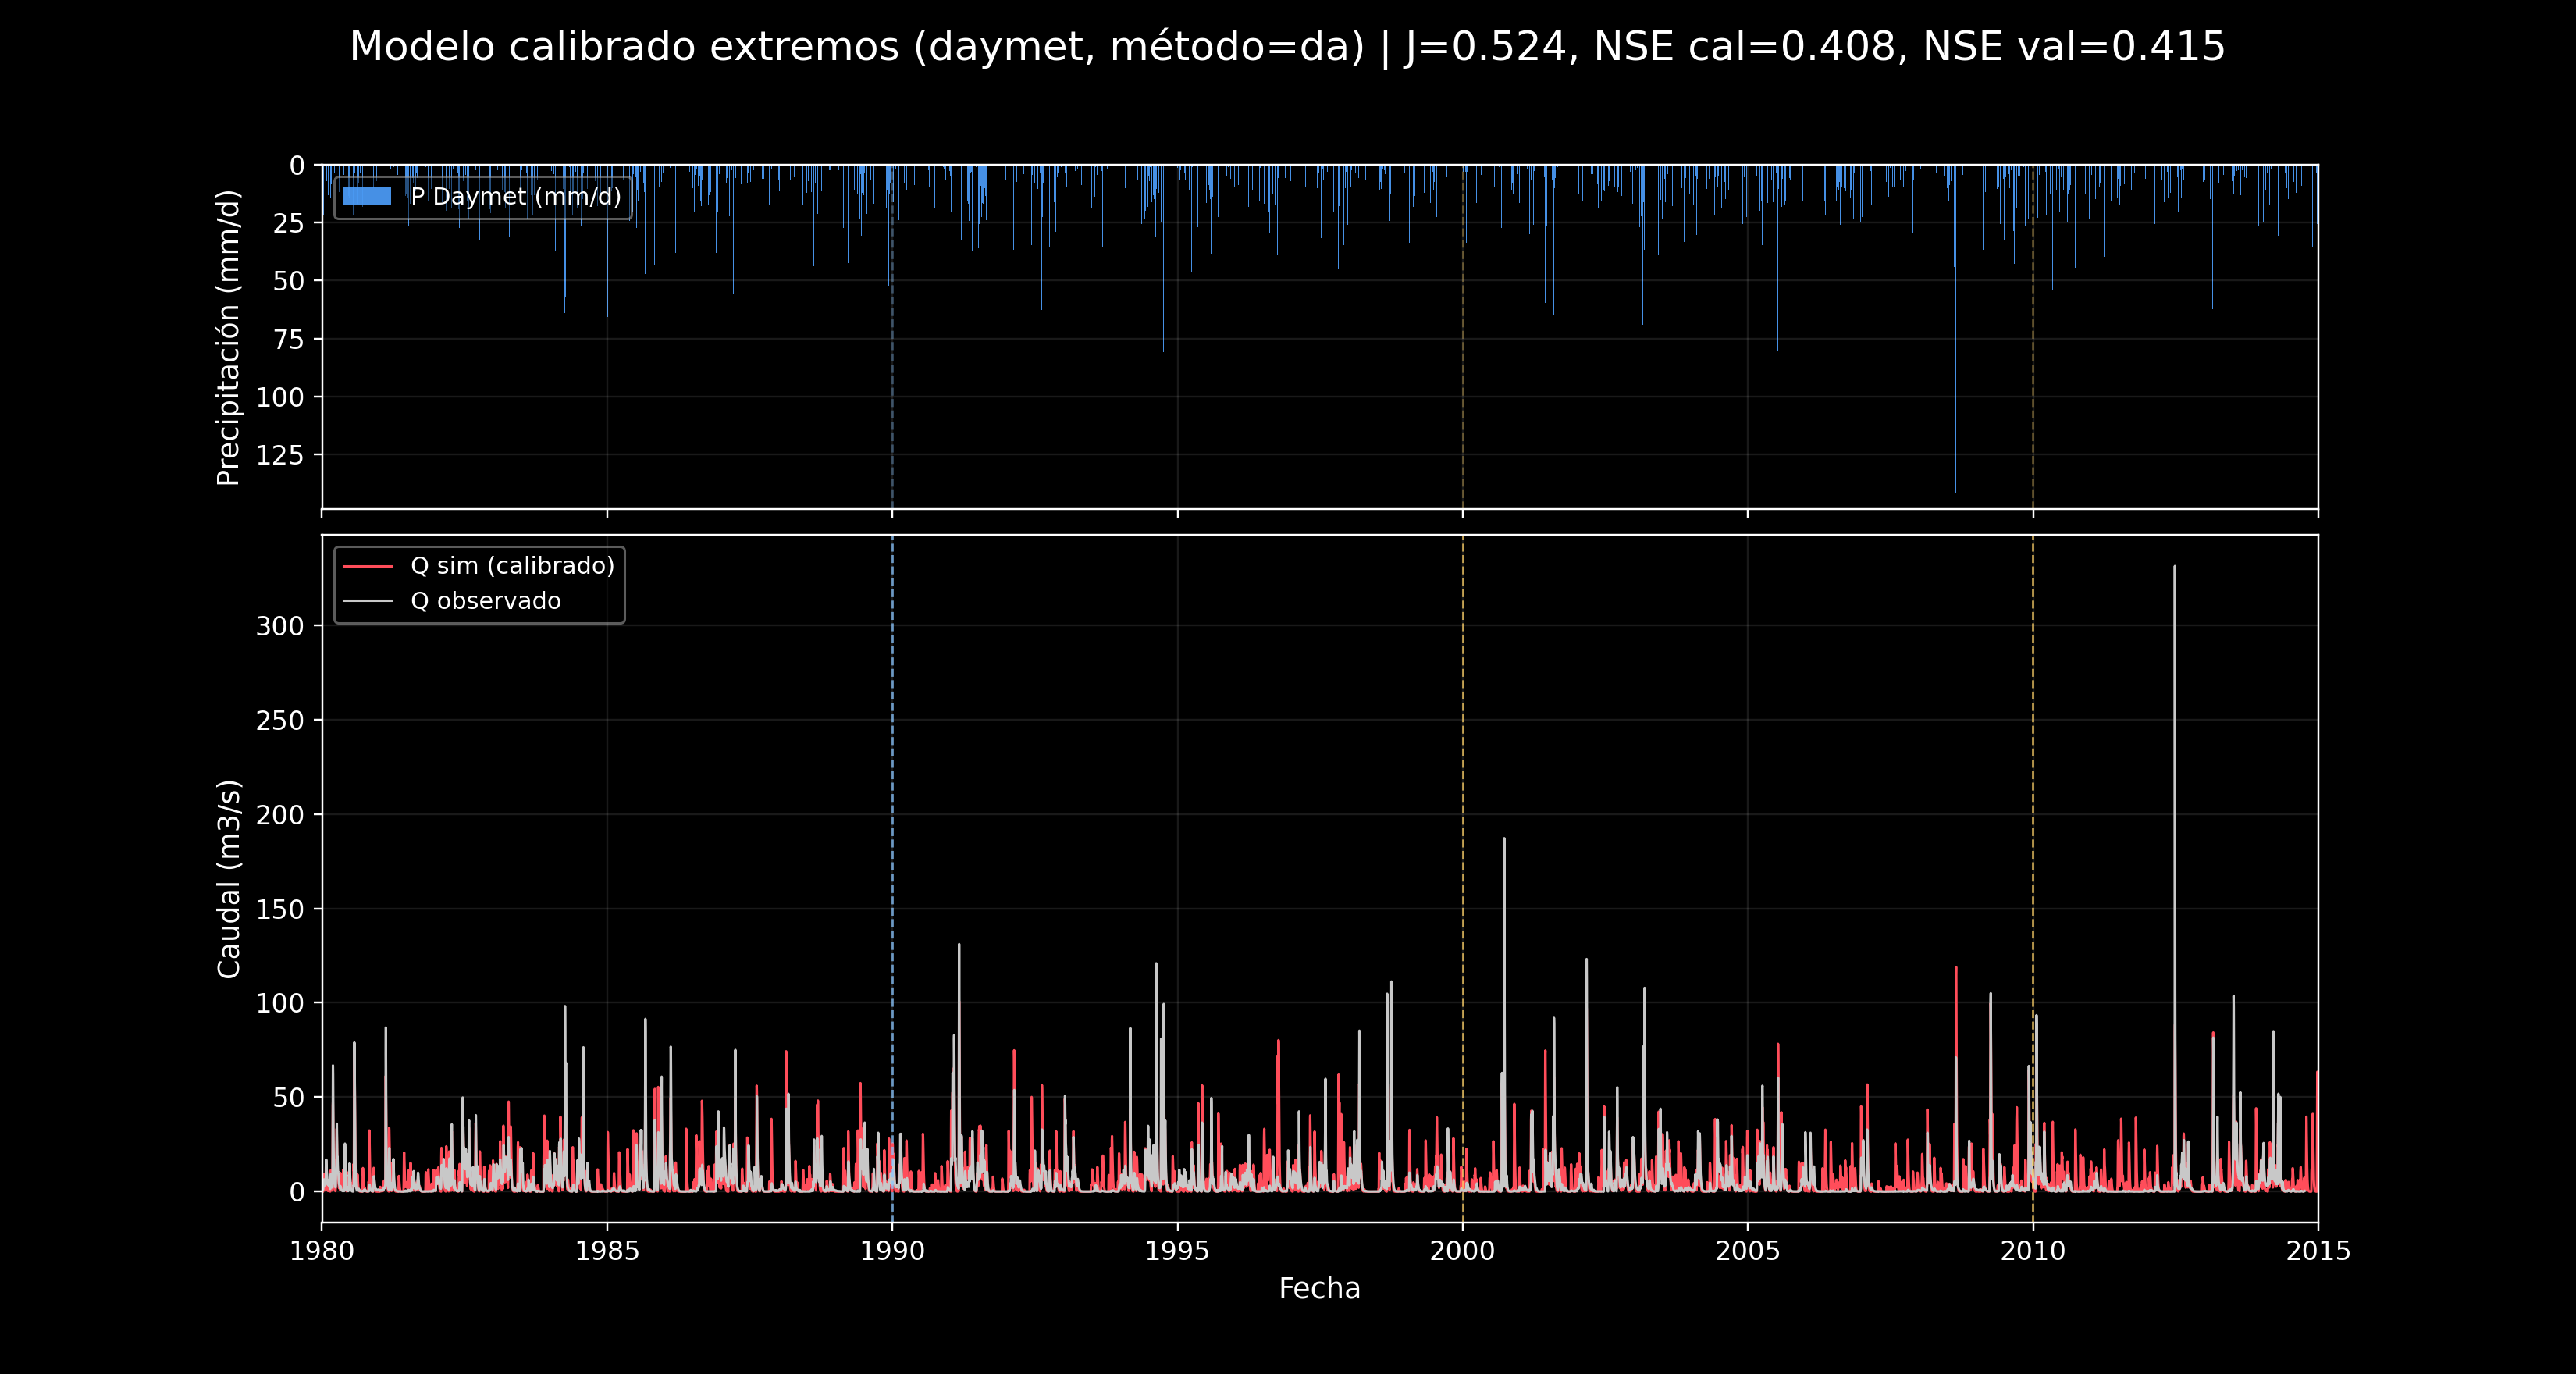
\includegraphics[width=0.48\textwidth]{../figuras/hidrograma_calibrado_extremos_daymet_da.png}
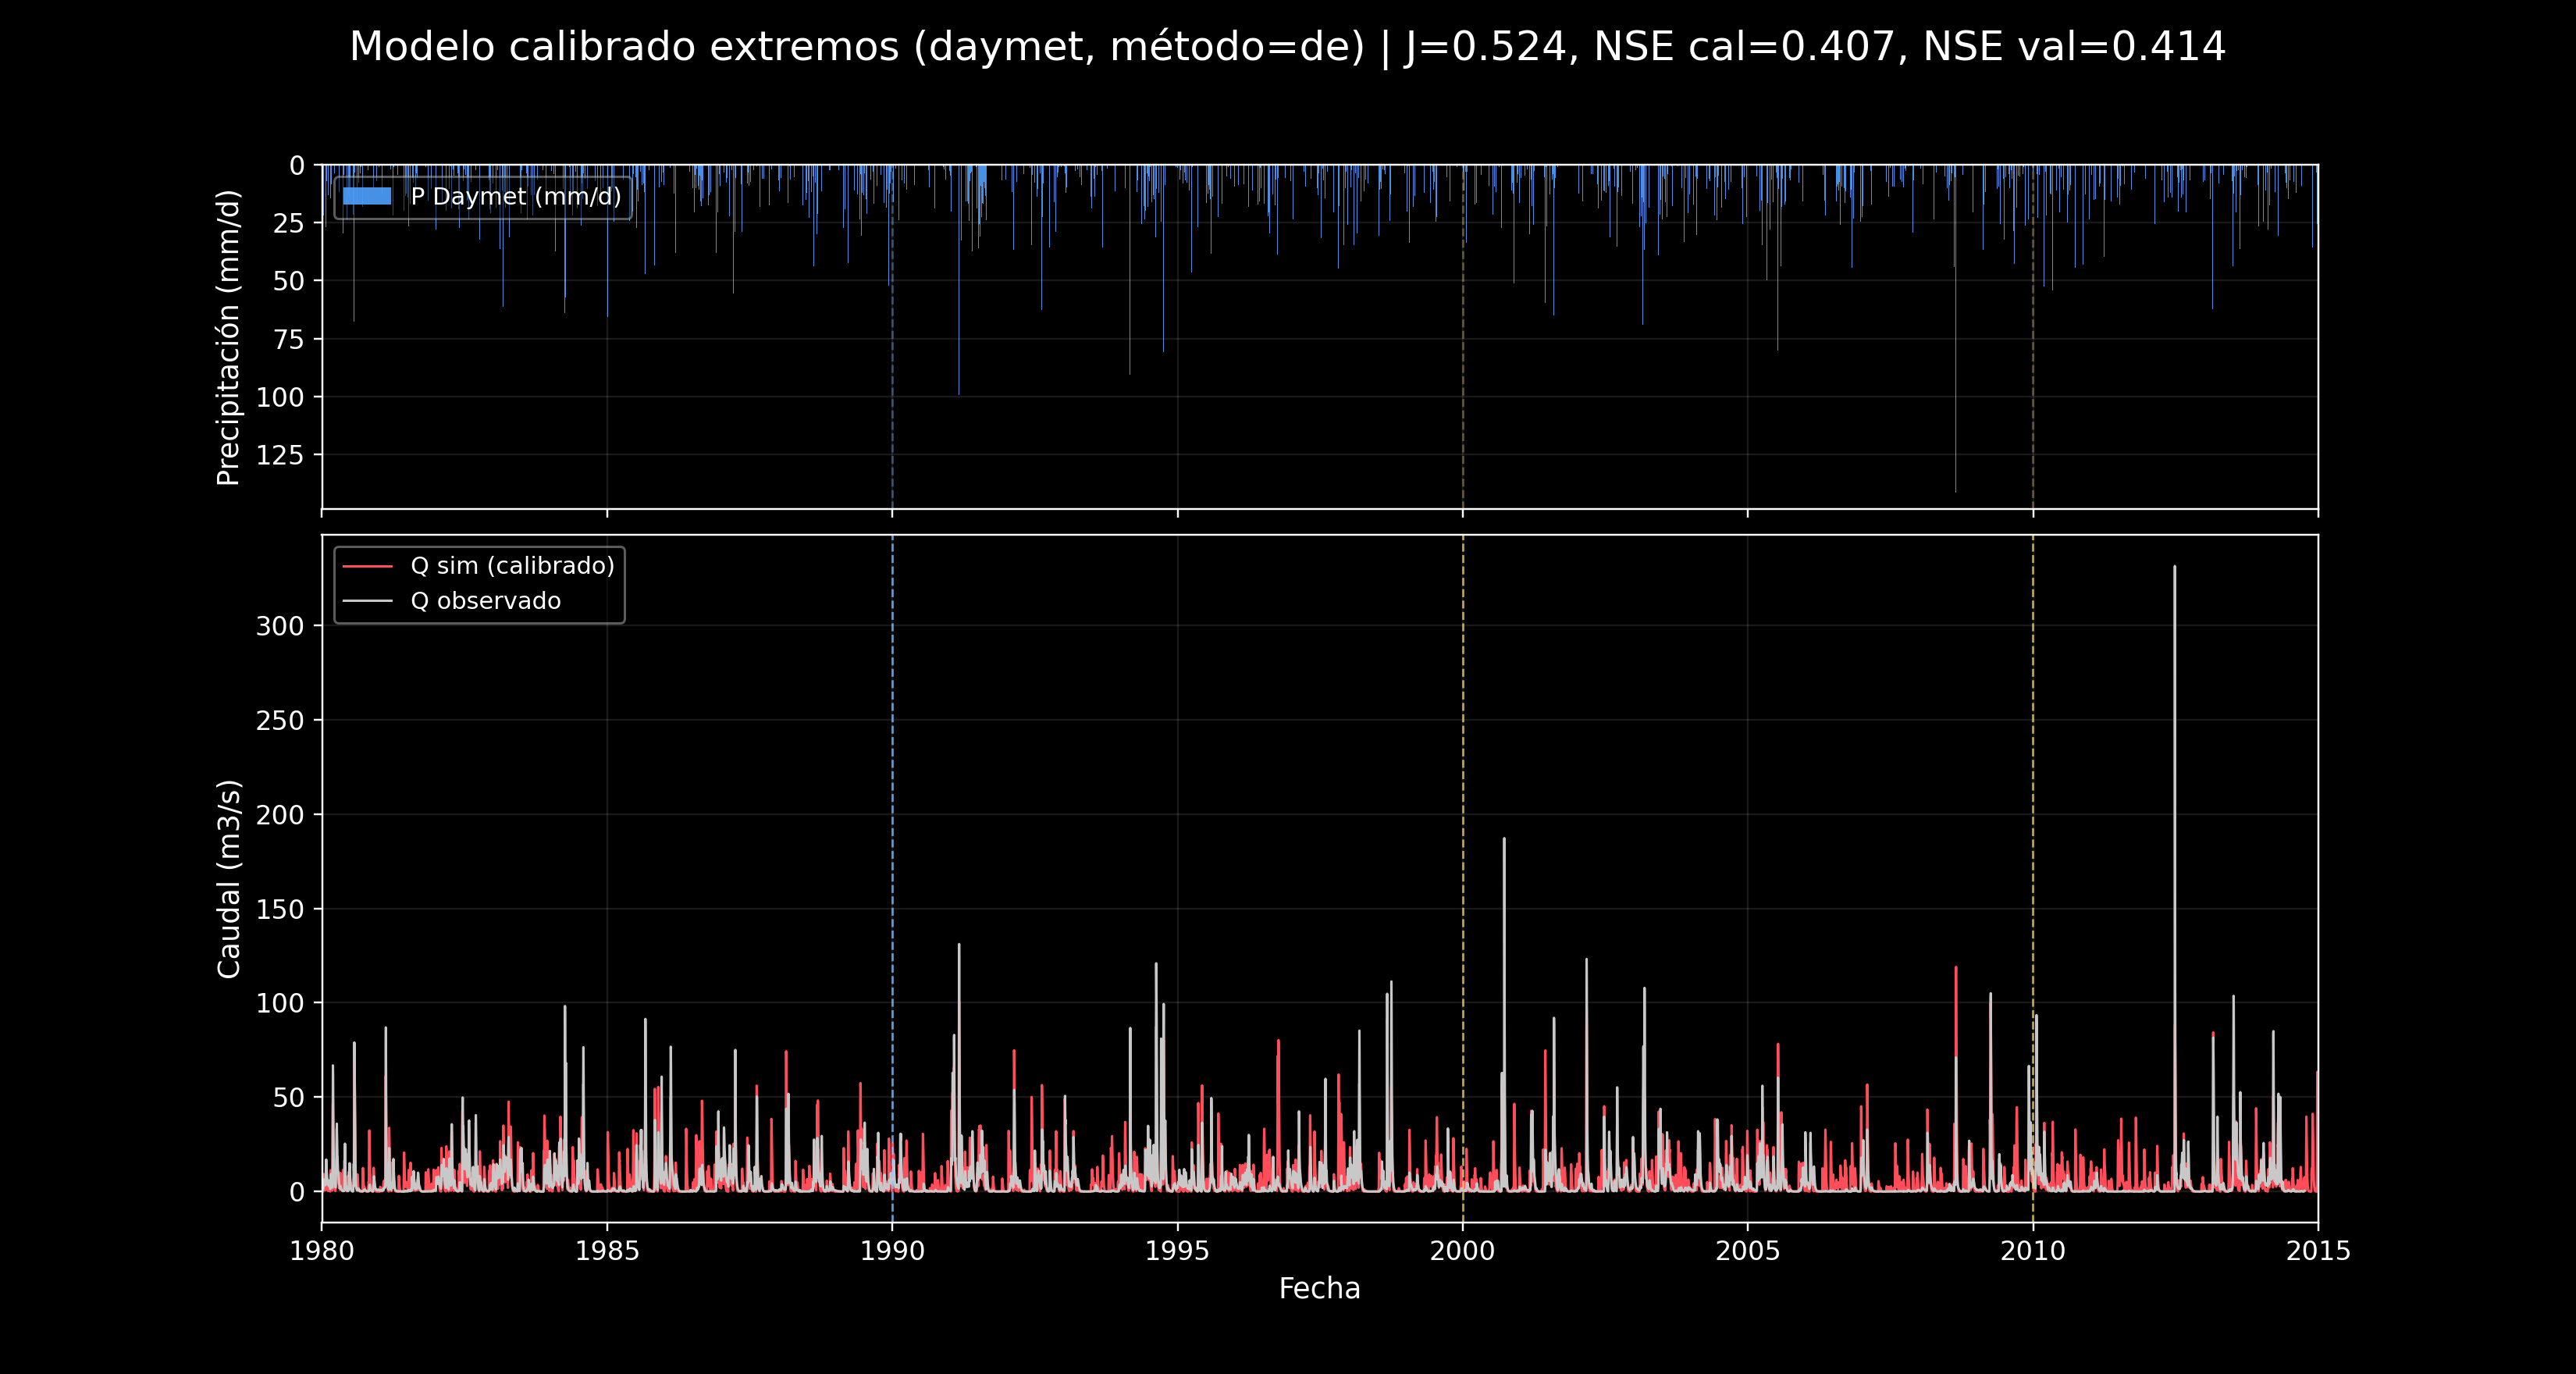
\includegraphics[width=0.48\textwidth]{../figuras/hidrograma_calibrado_extremos_daymet_de.png}
\caption{Calibrado extremos con Daymet (DA/DE).}
\end{figure}

\textbf{Desempeno con Daymet -- Extremos}

Para Daymet se obtuvo:
\begin{itemize}
\item $J_{cal} \approx 0.524$
\item $NSE_{cal} \approx 0.408$
\item $NSE_{val} \approx 0.415$
\end{itemize}

En comparacion con la mejor calibracion estandar, se observa una disminucion del NSE en validacion (de $\approx 0.603$ a $\approx 0.415$), lo cual evidencia el trade-off tipico de la calibracion orientada a extremos.

Visualmente, se aprecia una mejor representacion relativa de algunos picos de crecida, aunque aparecen episodios puntuales de sobreestimacion, coherentes con la penalizacion explicita por subestimacion incluida en la funcion objetivo.

\begin{figure}[H]
\centering
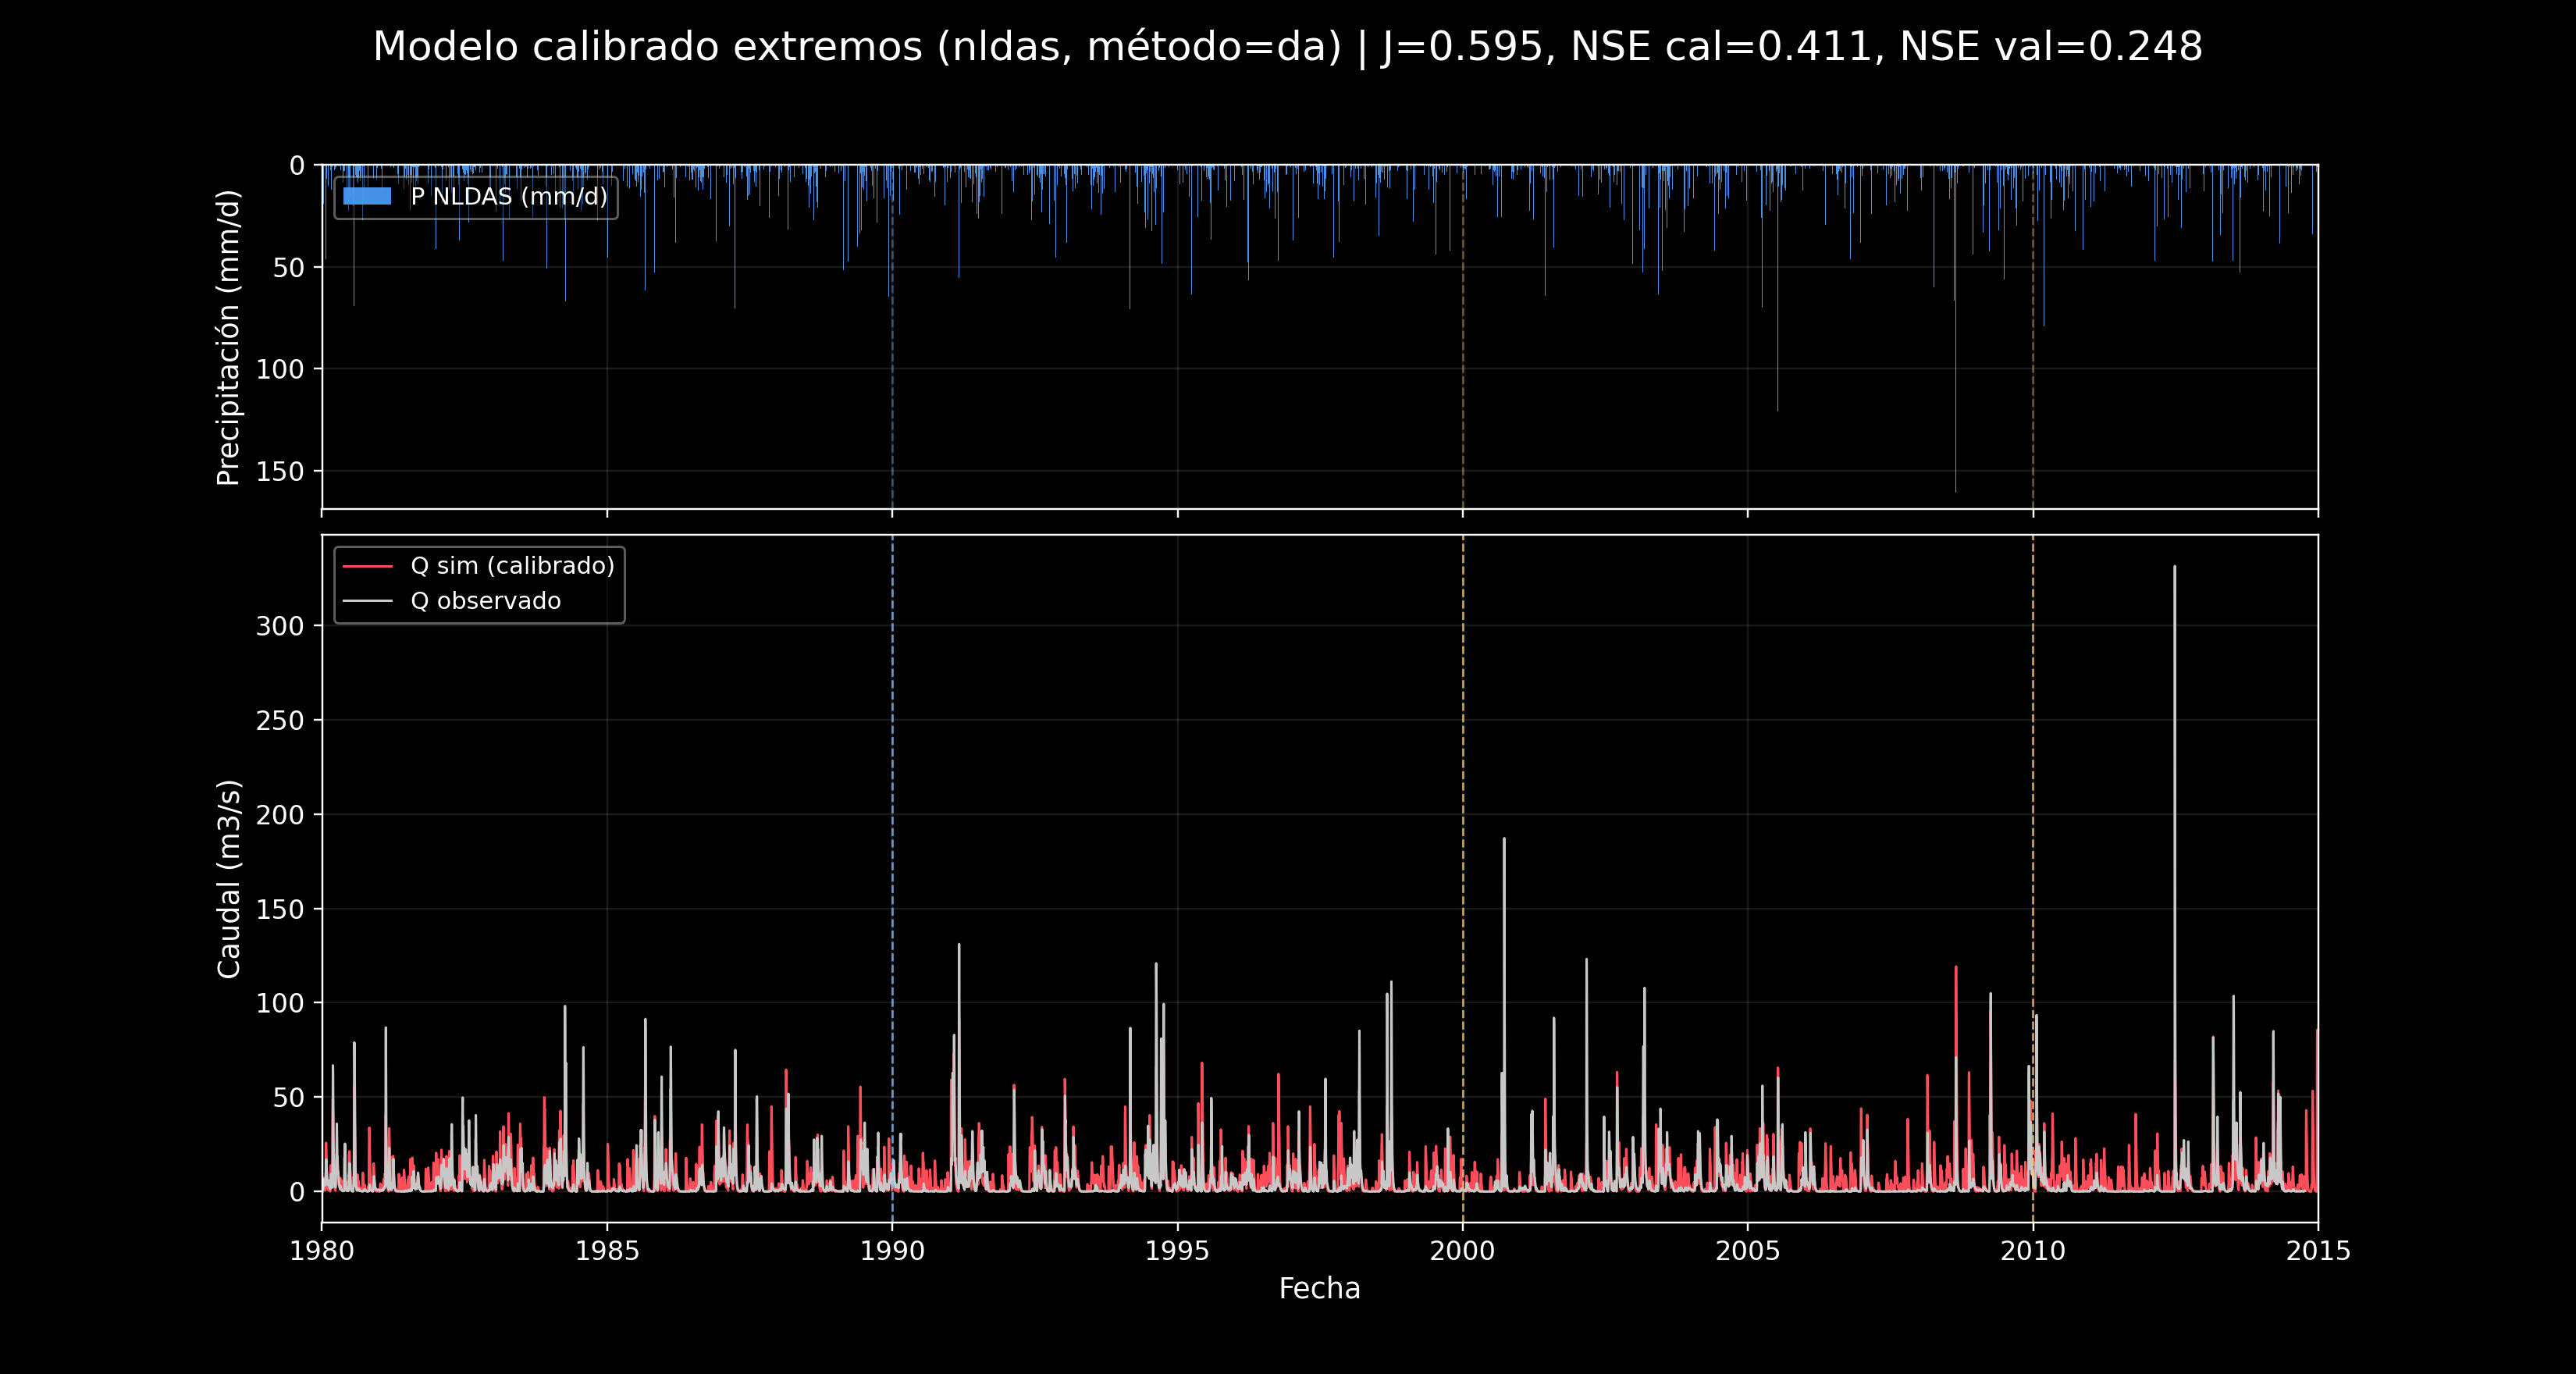
\includegraphics[width=0.48\textwidth]{../figuras/hidrograma_calibrado_extremos_nldas_da.png}
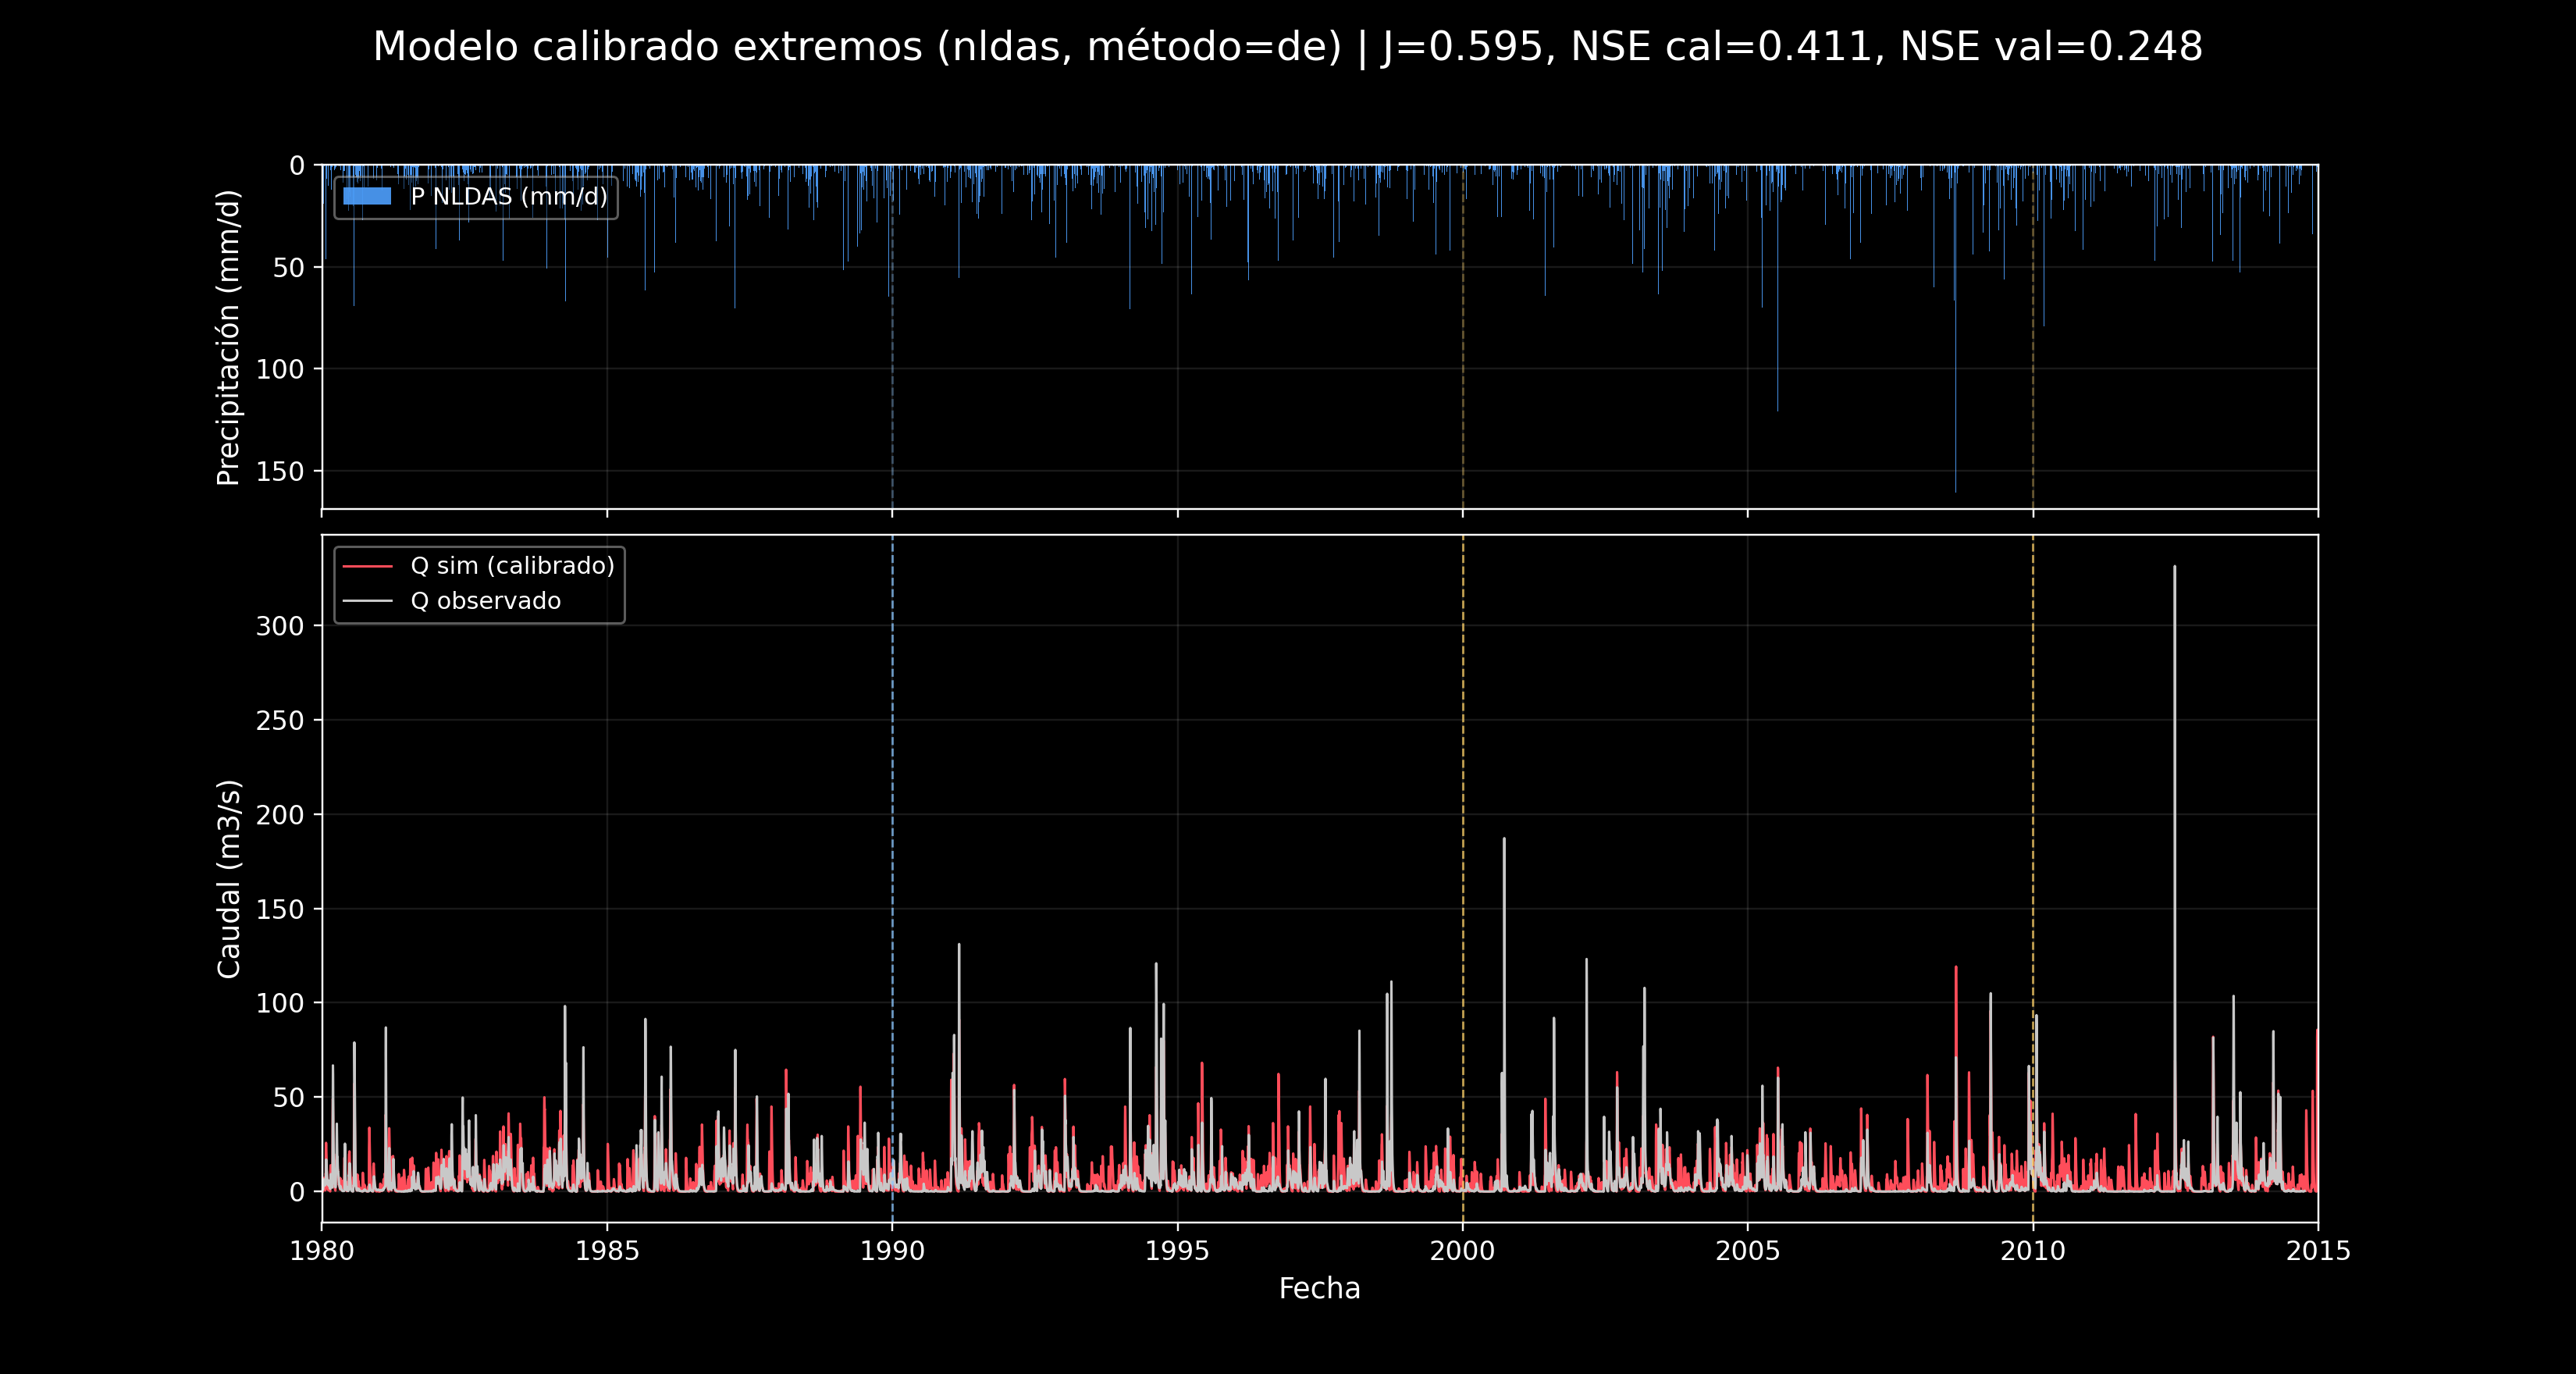
\includegraphics[width=0.48\textwidth]{../figuras/hidrograma_calibrado_extremos_nldas_de.png}
\caption{Calibrado extremos con NLDAS (DA/DE).}
\end{figure}

\textbf{Desempeno con NLDAS -- Extremos}

Para NLDAS se obtuvo:
\begin{itemize}
\item $J_{cal} \approx 0.595$
\item $NSE_{cal} \approx 0.411$
\item $NSE_{val} \approx 0.247$
\end{itemize}

Si bien el valor de $J$ es mayor que en Daymet, el desempeno en validacion medido por NSE es considerablemente inferior. Esto confirma que, aun bajo una funcion objetivo enfocada en crecidas, Daymet mantiene mayor robustez hidrologica general que NLDAS para esta cuenca.

\begin{table}[H]
        \centering
        \scriptsize
        \caption{Resultados calibración orientada a extremos}
        \label{tab:cal_ext}
        \resizebox{\textwidth}{!}{%
        \begin{tabular}{lllllllllllllllll}
\toprule
Fuente & Metodo & J\_cal & J\_val & NSE\_cal & NSE\_val & NSE\_high\_val & PeakBias\_val & UnderHigh\_val & ETc & beta & alpha1 & D1 & k1 & alpha2 & D2 & k2 \\
\midrule
daymet & da & 0.524 & 0.606 & 0.408 & 0.415 & 0.290 & 0.364 & 0.139 & 8.997 & 0.000 & 0.000 & 327.327 & 0.363 & 0.000 & 458.993 & 0.363 \\
daymet & de & 0.524 & 0.606 & 0.407 & 0.414 & 0.291 & 0.364 & 0.138 & 8.971 & 0.000 & 0.000 & 462.211 & 0.363 & 0.000 & 815.731 & 0.363 \\
nldas & da & 0.595 & 0.919 & 0.411 & 0.248 & -0.426 & 0.363 & 0.215 & 6.259 & 0.000 & 0.000 & 327.327 & 0.338 & 0.000 & 458.993 & 0.338 \\
nldas & de & 0.595 & 0.919 & 0.411 & 0.248 & -0.426 & 0.363 & 0.215 & 6.259 & 0.000 & 0.000 & 471.374 & 0.338 & 0.000 & 638.719 & 0.338 \\
\bottomrule
\end{tabular}

        }
        \end{table}

\begin{center}
\fcolorbox{cyan!50!black}{blue!20!black}{\parbox{0.94\textwidth}{
\textbf{La calibracion orientada a extremos mejora la representacion relativa de eventos de alto caudal, pero reduce el desempeno global medido por NSE.}

Este comportamiento evidencia un trade-off estructural del modelo conceptual: el ajuste promedio y la representacion optima de crecidas no pueden maximizarse simultaneamente bajo una misma configuracion parametrica.

La presencia de algunos picos sobreestimados no representa un error de implementacion, sino una consecuencia directa del criterio de optimizacion adoptado.
}}
\end{center}

\textbf{Consistencia de parametros y consideraciones fisicas}

Los parametros optimos permanecen dentro de los rangos establecidos. Sin embargo, se observa convergencia frecuente a valores de frontera:
\begin{itemize}
\item En calibracion estandar: $\alpha_1 \approx 0$ y $\alpha_2 \approx 0$
\item En calibracion de extremos: ademas $\beta \approx 0$
\end{itemize}

De acuerdo con la formulacion del modelo, esto implica:
\begin{itemize}
\item Ausencia de escorrentia directa ($\alpha_1 \approx 0$)
\item Ausencia de flujo rapido desde el tanque superior ($\alpha_2 \approx 0$)
\item Evapotranspiracion dependiente principalmente de $ET_c$ ($\beta \approx 0$)
\end{itemize}

Esta configuracion favorece una respuesta mas amortiguada y controlada por almacenamiento, lo cual es consistente con la estructura del modelo y con la subestimacion parcial de ciertos picos observada en los hidrogramas.

{\Large\textbf{\textcolor{cyan}{Validacion del modelo (2000--2009)}}}

La validacion del modelo se realizo sobre el periodo independiente 2000--2009, evaluando la capacidad de generalizacion fuera del intervalo de calibracion (1990--1999).

El desempeno se analizo mediante tres enfoques complementarios:
\begin{enumerate}
\item analisis temporal del hidrograma,
\item diagrama de dispersion $Q_{obs}$ vs $Q_{sim}$,
\item curva de duracion de caudales (FDC).
\end{enumerate}

\begin{figure}[H]
\centering
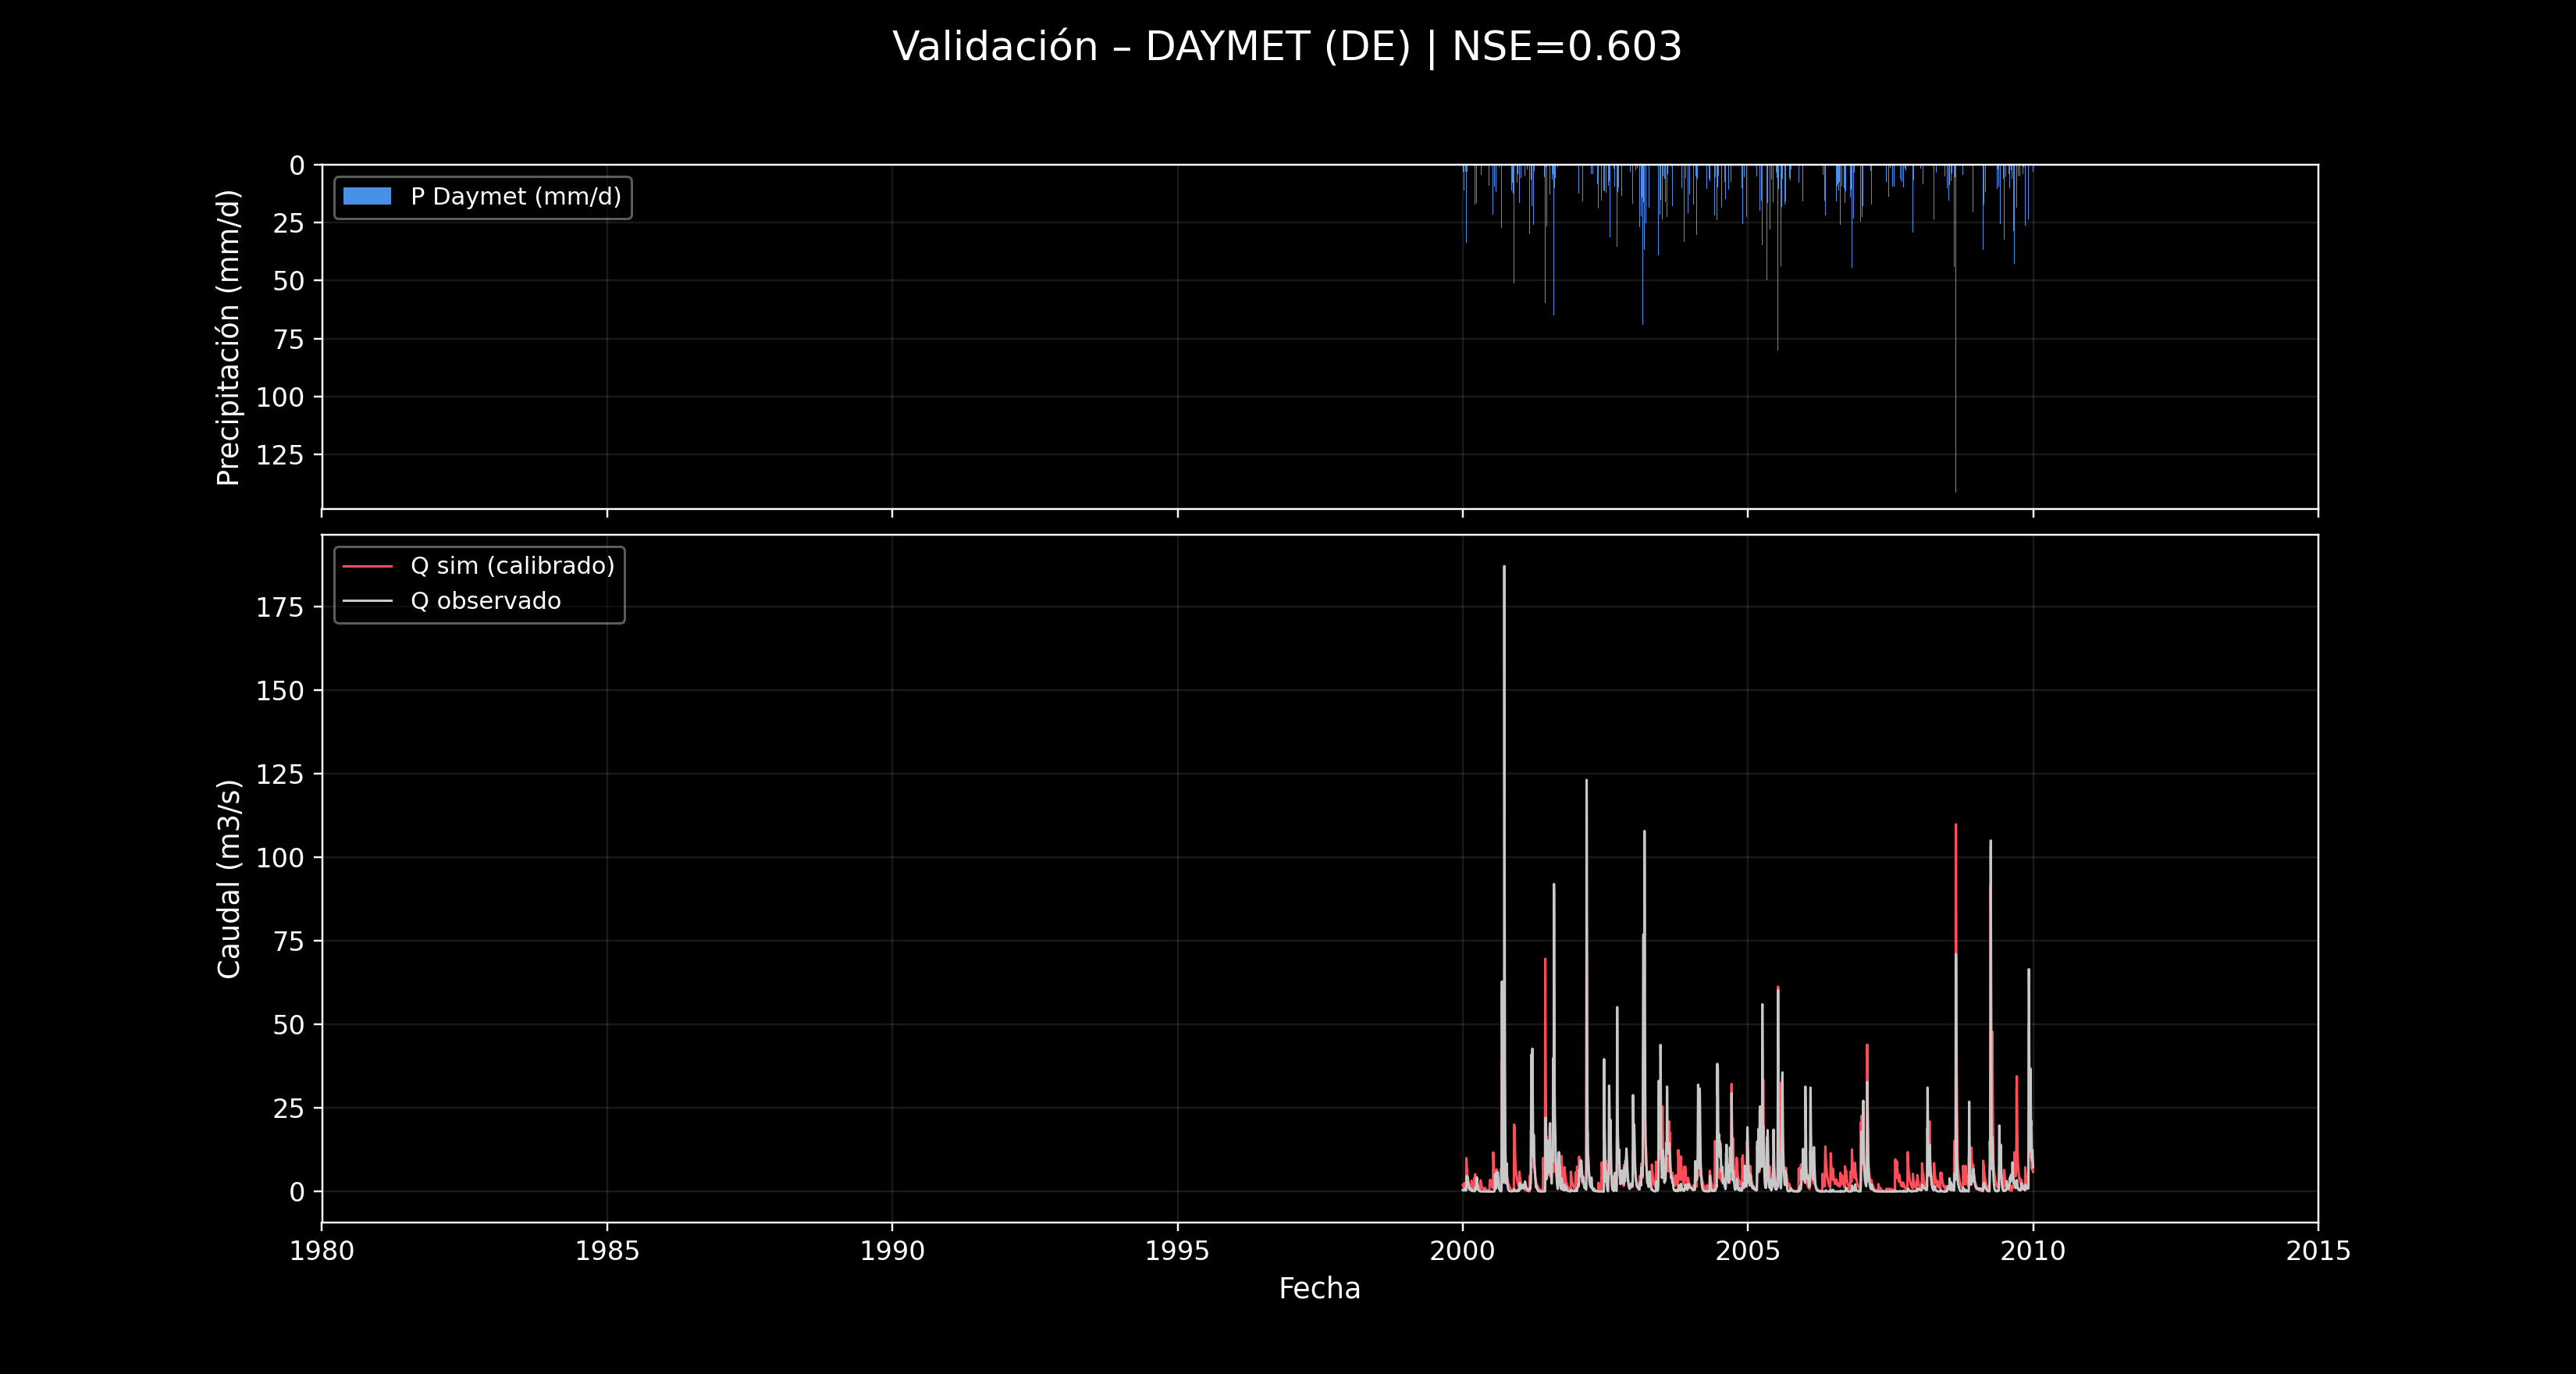
\includegraphics[width=0.95\textwidth]{../figuras/validacion.png}
\caption{Validacion (hidrograma interactivo, version estatica para PDF).}
\end{figure}

El hidrograma de validacion muestra que el modelo reproduce adecuadamente la dinamica temporal de los eventos, capturando la ocurrencia de crecidas y la variabilidad intra-anual.

La configuracion estandar con Daymet (DE) presenta el mejor desempeno global ($NSE_{val}=0.603$), evidenciando buena capacidad de generalizacion.

No obstante, se observa una tendencia sistematica a subestimar algunos picos de alta magnitud, especialmente en eventos extremos, lo cual es consistente con el comportamiento estructural identificado durante la calibracion.

Graficas interactivas complementarias: \texttt{\detokenize{figuras/html/validacion_scatter_obs_vs_sim.html}} y \texttt{\detokenize{figuras/html/validacion_fdc_obs_vs_sim.html}}.

\textbf{Interpretacion de la dispersion $Q_{obs}$ vs $Q_{sim}$}

El diagrama de dispersion confirma el patron observado en el hidrograma.
\begin{itemize}
\item La mayoria de los puntos correspondientes a caudales altos se ubican por debajo de la linea 1:1, indicando subestimacion estructural de crecidas.
\item En caudales bajos se observa mayor dispersion relativa, comportamiento tipico de modelos conceptuales de baja complejidad.
\end{itemize}
La configuracion estandar con Daymet presenta la menor dispersion global y mayor concentracion alrededor de la linea 1:1, lo que confirma su mayor estabilidad en validacion.

\textbf{Interpretacion de la FDC observada vs simulada}

La FDC permite evaluar la representacion estadistica del regimen hidrologico completo.

La probabilidad de excedencia indica el porcentaje del tiempo en que un determinado caudal es igualado o superado.
\begin{itemize}
\item Valores bajos de excedencia representan eventos de alta magnitud.
\item Valores altos corresponden a caudales bajos o de base.
\end{itemize}

Se observa que la calibracion estandar con Daymet reproduce de forma mas consistente la forma de la curva observada en la mayor parte del rango de probabilidades.

Las calibraciones orientadas a extremos muestran mejor ajuste relativo en la zona de bajas excedencias (altos caudales), pero mayor divergencia en caudales medios y bajos, confirmando el trade-off previamente discutido.

\section*{Analisis y discusion}
\textbf{Discusion comparativa de estrategias de calibracion}

La comparacion entre fuentes meteorologicas (Daymet y NLDAS), metodos de optimizacion (DE y DA) y funciones objetivo (NSE estandar vs funcion orientada a extremos) permite identificar los factores que mas influyen en el desempeno del modelo de dos tanques.

\textbf{Influencia de la fuente meteorologica}

Daymet supera consistentemente a NLDAS en validacion. En calibracion estandar, Daymet obtiene $NSE_{val}$ entre 0.567 y 0.603, mientras que NLDAS obtiene valores entre 0.388 y 0.396.

La diferencia se confirma en:
\begin{itemize}
\item Hidrograma (mejor ajuste visual)
\item Dispersion $Q_{obs}$--$Q_{sim}$ (menor sesgo)
\item FDC (mejor representacion del regimen completo)
\end{itemize}

Esto indica que la calidad y resolucion espacial del forzamiento meteorologico es el factor mas influyente en el desempeno del modelo para esta cuenca.

\textbf{Influencia del metodo de optimizacion}

La influencia del optimizador es secundaria frente a la fuente meteorologica, aunque DE mejora el NSE de validacion de Daymet de 0.567 a 0.603. Para NLDAS la diferencia entre metodos es menor (0.388--0.396).

Esto sugiere que:
\begin{itemize}
\item Ambos algoritmos encuentran soluciones hidrologicamente competitivas.
\item Las diferencias parametricas evidencian equifinalidad.
\item El metodo de optimizacion tiene menor impacto que la calidad del forzamiento.
\end{itemize}

\textbf{Calibracion estandar vs calibracion orientada a extremos}

La calibracion estandar maximiza el ajuste global (NSE) y produce el mejor desempeno general.

La calibracion orientada a extremos mejora parcialmente la representacion de picos, pero reduce el NSE global (Daymet $NSE_{val} \approx 0.415$; NLDAS $\approx 0.247$).

Esto evidencia un \textbf{trade-off} estructural:
\begin{itemize}
\item Mejor ajuste de crecidas
\item A costa de perdida de ajuste promedio
\end{itemize}

La FDC muestra que la calibracion estandar reproduce mejor la distribucion completa, mientras que la calibracion de extremos altera la cola baja y aumenta la dispersion.

\textbf{Interpretacion fisica de los parametros calibrados}

La convergencia frecuente de parametros a valores en frontera ($\alpha_1 = 0$, $\alpha_2 = 0$ y $\beta = 0$ en calibracion de extremos) tiene una interpretacion hidrologica clara.
\begin{itemize}
\item $\alpha_1 = 0$ implica ausencia de escorrentia directa inmediata.
\item $\alpha_2 = 0$ indica ausencia de flujo rapido desde el primer tanque.
\item $\beta = 0$ sugiere evapotranspiracion controlada principalmente por $ET_c$, sin dependencia directa de la lluvia diaria.
\end{itemize}

En conjunto, los resultados sugieren una cuenca dominada por almacenamiento y liberacion gradual, con respuesta relativamente amortiguada frente a eventos de lluvia.

Este comportamiento es coherente con la subestimacion parcial de picos observada en validacion.

{\Large\textbf{Limitaciones del modelo}}

El modelo conceptual de dos tanques presenta limitaciones inherentes a su estructura simplificada:
\begin{itemize}
\item No representa procesos fisicos explicitos ni heterogeneidad espacial.
\item Tiende a subestimar eventos extremos de alta magnitud.
\item Presenta parametros en frontera, lo que sugiere flexibilidad estructural limitada.
\item Es altamente sensible a la calidad del forzamiento meteorologico.
\item Puede existir equifinalidad (multiples combinaciones parametricas con desempeno similar).
\end{itemize}

En consecuencia, el modelo representa adecuadamente el comportamiento agregado del sistema, pero simplifica la complejidad hidrologica real.

{\Large\textbf{Propuestas de mejora}}

Para fortalecer la capacidad predictiva del modelo se proponen:
\begin{itemize}
\item Implementar calibracion multiobjetivo (NSE global + metricas de extremos).
\item Incorporar un componente explicito de escorrentia rapida.
\item Evaluar estructura con almacenamiento adicional.
\item Realizar analisis de sensibilidad e incertidumbre.
\item Explorar correccion o combinacion de fuentes meteorologicas.
\end{itemize}

Estas mejoras permitirian reducir el compromiso entre ajuste global y representacion de crecidas.

\section*{Conclusion general}
El modelo conceptual de dos tanques implementado para la cuenca Sopchoppy logra un cierre robusto del balance hidrico y reproduce razonablemente la dinamica lluvia--escorrentia.

La evaluacion comparativa demuestra que:
\begin{itemize}
\item La fuente meteorologica es el factor mas determinante en el desempeno.
\item Daymet ofrece mayor generalizacion; la mejor configuracion obtiene $NSE_{val} \approx 0.603$.
\item El metodo de optimizacion tiene un impacto secundario, con ventaja de DE para Daymet.
\item La calibracion orientada a extremos mejora parcialmente la representacion de crecidas, pero reduce el desempeno global.
\end{itemize}

El analisis integrado mediante hidrogramas, dispersion y FDC confirma que la configuracion Daymet--DE con calibracion estandar ofrece el mejor equilibrio entre coherencia fisica, estabilidad numerica y capacidad predictiva.

La presencia de parametros en frontera sugiere una cuenca dominada por almacenamiento lento, consistente con el comportamiento hidrologico observado.

En sintesis, el modelo constituye una herramienta adecuada para simulacion hidrologica general en esta cuenca, aunque futuras mejoras estructurales y estrategias multiobjetivo podrian fortalecer la representacion de eventos extremos.

\end{document}
